%!TEX root = ../../dissertation.tex
%%%%%%%%%%%%%%%%%%%%%%%%%%%%%%%%%%%%%%%%%%%%%%%%%%%%%%%%%%%%%%%%%%%%%%%%%%%%%%%%
\chapter{Mobile Core Network Investigation}
\label{chap:mobilenets}


%% NEW
This chapter is structured as follows.

\begin{itemize}
\item Technical Background. Standard Organisations. Network Architecture. Protocol Details.
\item Dataset Description. Methodology.
\item Evaluations. Dataset Analysis. Statistics. Traffic Characteristics. How does that user traffic fit in?
\item Definition of Load etc
\item Fitting, Modeling and Simulation
\item Summary
\end{itemize}

Core is usually neglected in communication investigations

But 




%%%%%%%%%%%%%%%%%%%%%%%%%%%%%%%%%%%%%%%%%%%%%%%%%%%%%%%%%%%%%%%%%%%%%%%%%%%%%%%
\section{Introduction}
\label{c4:sec:introduction}


The Internet has reached ubiquity some time ago. When there is no wired access nearby you can rely on WiFi hotspots and cellular networks for wide area coverage. These cellular networks are usually based on \ac{3GPP} specifications which have evolved from the circuit switched \ac{GSM} network into the fully packet switched \ac{LTE} which is still in its unrolling phase. But being packet switched does not mean that it shares a lot of similarity with a typical wireline Internet protocol stack and network infrastructure. A ``3G'' network (a term synonymous for the typical type of cellular network used today) is very distinct from typical wired networks as it must provide, amongst others, mobility and authentication in its core specifications rather than being optional on-top services as is typically used in the Internet.

The TCP/IP stacks largely follows two principles: \ac{KISS} and the end-to-end principle\cite{saltzer1984end2end}, which essentially means to restrict the protocols to the necessary bare-minimum and keep state only in the end systems. 3G takes a different approach, keeps a large amount of state at the obligatory nodes in its ``core network'', which explicitly communicate by signaling procedures defined by the \ac{3GPP}.
The adverse effects of state-keeping in network devices have been known to, e.g.,  Internet users running BitTorrent across low-end home routers as of the early 2000s. In \ac{UMTS} mobile networks, the networking hardware is vastly more powerful, but the control plane tasks are vastly more complex than port and network translation as well, namely carrying and routing IP and voice traffic, user mobility, \ac{AAA} and so on. Many specialized protocols are involved to communicate intents and states in the network. This causes processing overhead, additional traffic on network paths, and increases the number of states to be held in memory on the core network nodes. All of these attributes can be subsumed under the term network ``load'' which we plan to investigate in this work.

While other publications look at the near-edge interactions in these network, research on the core is scarce, the reason for it being simple: you cannot do research without data from the operator there. Research at the edge, beginning at the IP stack level and upwards, can be conducted relatively simple. Writing simple tests and measurement scripts, often involving tcpdump and other tools, is usually all you need. But a mobile phone doesn't let you peek inside its layer 1 and 2 interactions (or even the implementation). Any information on this black box must be indirectly inferred from above (forcing behavior known from the specifications through scripts) or below (spectrum analysis using software defined radio approaches). To take a look at the core's view of traffic and data, one needs access to a dedicated measurement and capturing infrastructure placed inside the network. With this, researchers can not just look into user traffic flowing through the network but also quite easily into the signaling heavy mobile network control plane. 

Operators usually dimension their networks in relation to the occurring user traffic. But in such a signaling-dependent architecture this might not hold true anymore, as every user traffic has to be explicitly allowed, set up, and metered through all of the network's components. This has already led to some troubles in some mobile access networks, as heavy signaling for user traffic tunnels with very small amounts of traffic, that were however closed and reopened at a very high rate, caused an unintended \ac{DDoS} in the radio access network\cite{lt2012docostorm, it2011birdandroid}. 
This inherent complexity of signaling in mobile cellular networks is easily missed by programmers who do not or cannot know that their applications will run over such wireless links, and probably would not expect it from a network that pretends to transparently carry IP.

In this publication we attempt to give some insights into the mobile network control plane and its impact on dimensioning and load modeling. To do this, some important aspects of the \ac{3GPP} specifications have to be explained to give some basic vocabulary for the following exploratory research into signaling with a focus on \ac{PDP} Contexts and their management through \ac{GTP} tunnel management procedures. Using a week long data set from an Austrian mobile operator recorded at the Gn interface between the \ac{SGSN} and \ac{GGSN}, we attempt to find criteria influencing the signaling but we are also formulating hypotheses on the load impact of signaling, both backed by statistics gathered from the the data set.\\



%%%%%%%%%%%%%%%%%%%%%%%%%%%%%%%%%%%%%%%%%%%%%%%%%%%%%%%%%%%%%%%%%%%%%%%%%%%%%%%%
%% CoNEXT Intro starts here

Given its roots as a research network and its growing pervasiveness over the last forty years, it is understandable that research on the Internet covers all parts of the network from applications to access to the core, and has been going on ever since what could be considered prehistoric times of the Net. The state of research on mobile cellular networks such as 3G is lean in comparison. Mobile networks providing Internet access have not been around for too long, and still are not available in all parts of the world. Furthermore, most research focuses on user-oriented metrics such as traffic statistics and mobility patterns, or takes into account the radio part of the network only. Little has been published about activity within the core network, and yet less about signaling.

Given how limited spectral resources on the radio interface are, it might not seem obvious to think about signaling load in the network. Yet, there have been situations where the core network unintentionally has been flooded with signaling, taking down user-plane connectivity on the way, despite small amounts of actual user traffic being transported \cite{lt2012docostorm, it2011birdandroid}. 

The adverse effects of state-keeping in network devices have been known to, e.g.,  Internet users running BitTorrent across low-end home routers as of the early 2000s. In \ac{UMTS} mobile networks, the networking hardware is vastly more powerful, but the control plane tasks are vastly more complex than port and network translation as well, namely carrying and routing IP and voice traffic, user mobility, \ac{AAA} and so on. Many specialized protocols are involved to communicate intents and states in the network. This causes processing overhead, additional traffic on network paths, and increases the number of states to be held in memory on the core network nodes. Therefore, in scenarios such as the ones mentioned above, radio access is not the bottleneck to connectivity any more, but signaling is.

The inherent complexity of signaling in mobile cellular networks is easily missed by programmers who do not or cannot know that their applications will run over such wireless links, and probably would not expect it from a network that pretends to transparently carry IP. What furthers this problem is the lack of literature on the theoretical and practical sides of these issues.

This apparent lack is due to a number of reasons. First, gaining sufficiently intimate knowledge on the huge corpus of \ac{3GPP} Technical Specifications %\ac{TS}
is a laborious task. Second, to come up with lower-layer measurements requires physical access to the core network infrastructure and suitable measurement equipment. Also, much of the data is commercially and privacy-sensitive, and cannot be published without extensive sanitizing.

The purpose of this paper will therefore be to give a 3G tunnel management primer, introducing the relevant \acs{GPRS}/\acs{UMTS} network structure and the involved control plane protocols with a special focus on the \ac{GTP}, which is probably the most prevalent. % We discuss how much overhead is put on the network through \ac{GTP} in a typical user traffic scenario.
Furthermore, we share our first insights into one practical aspect of the signaling process, the \ac{GTP} tunnel management procedures. Using a week long data set from an Austrian mobile operator recorded at the Gn interface between the \ac{SGSN} and \ac{GGSN}, % by the \ac{METAWIN} measurement infrastructure from the FTW, 
we take a look at \ac{PDP} Context durations, i.e. the time a \ac{PDP} Context is established and held, argue how this influences the load on the network, and evaluate the data by device types and operating systems.

Our measurement data backs up a number of straightforward assumptions on the behavior of different device and operating system types, but also reveals some remarkable differences in tunnel characteristics.\\





%%%%%%%%%%%%%%%%%%%%%%%%%%%%%%%%%%%%%%%%%%%%%%%%%%%%%%%%%%%%%%%%%%%%%%%%%%%%%%%%
\section{Background}

%%%%%%%%%%%%%%%%%%%%%%%%%%%%%%%%%%%%%%%%%%%%%%%%%%%%%%%%%%%%%%%%%%%%%%%%%%%%%%%%
\subsection{Standards and Standards Bodies}

Point out the Standards organizations responsible for mobile networks and the differences to / conflicts with other areas, especially the Internet

Compare \ac{3GPP} \acp{TS} with \ac{IETF} \acp{RFC} in terms of accessibility, size, technical clarity and what this means for the market and implementors (scarce number, because no one really understands TSs, only now \ac{FOSS} implementations of \ac{GSM} (barely \ac{GPRS}))

Conclude, that this pretty much hinders and closes any competitive market and innovation (not by committee) by few major players

\ac{IETF}+\ac{ISOC}+\ac{IAB}+? on Internet site
\ac{ISO}+\ac{ETSI}+? old school standards by committee, closed standards
\ac{ITU}+\ac{3GPP}+? mobile standards
\ac{IEEE}




%%%%%%%%%%%%%%%%%%%%%%%%%%%%%%%%%%%%%%%%%%%%%%%%%%%%%%%%%%%%%%%%%%%%%%%%%%%%%%%%
% describe anything related to 3gpp architectures, protocol,
% and signaling basics here
%!TEX root = dissertation.tex
%%%%%%%%%%%%%%%%%%%%%%%%%%%%%%%%%%%%%%%%%%%%%%%%%%%%%%%%%%%%%%%%%%%%%%%%%%%%%%%%
%
% Collection of all relevant mobile radio specifications and descriptions
%
\section{Übersicht}

\begin{itemize}
\item Einarbeitung
	\begin{itemize}
		\item Architektur von 3G-Netzen
		\item Modelle zur Beschreibung von Datenverkehrsflüssen
		\item Einarbeitung in das Messsystem des FTW
	\end{itemize}
\item Definition eines einfachen Bearer-Modells
\item Programmierung der Auswertung
\item Durchführung und Auswertung der Messungen
\item Anfertigung eines Berichtes
\end{itemize}

\section{Modeling}
Macroscopic Behavior

	-- time Connection Setup until Call Termination with Talk Spurts
	--> ON/OFF Process
	--> Empricial measurement
	
Source Traffic Model
	-- 2 parts: 
		arrival process for user activities
		process describing activity phase
	-- arrival time:
		User begins web browsing
	
Simulation \& Software
	ns-2 UMTS mobile parts only
	ns-3 GSoC2010 implementing \ac{UTRAN} (MAC\&PHY) incl radio bearers (+OpenFlow)
	Harald Welte GPRS: OpenBSC, OpenGGSN incl GTP
	

EPS first introduced in 3GPP Release 8, completed in March 2009. Consisting of EUTRAN, EPC (formerly SAE)


	


\begin{figure}[htbp]
 \centering
 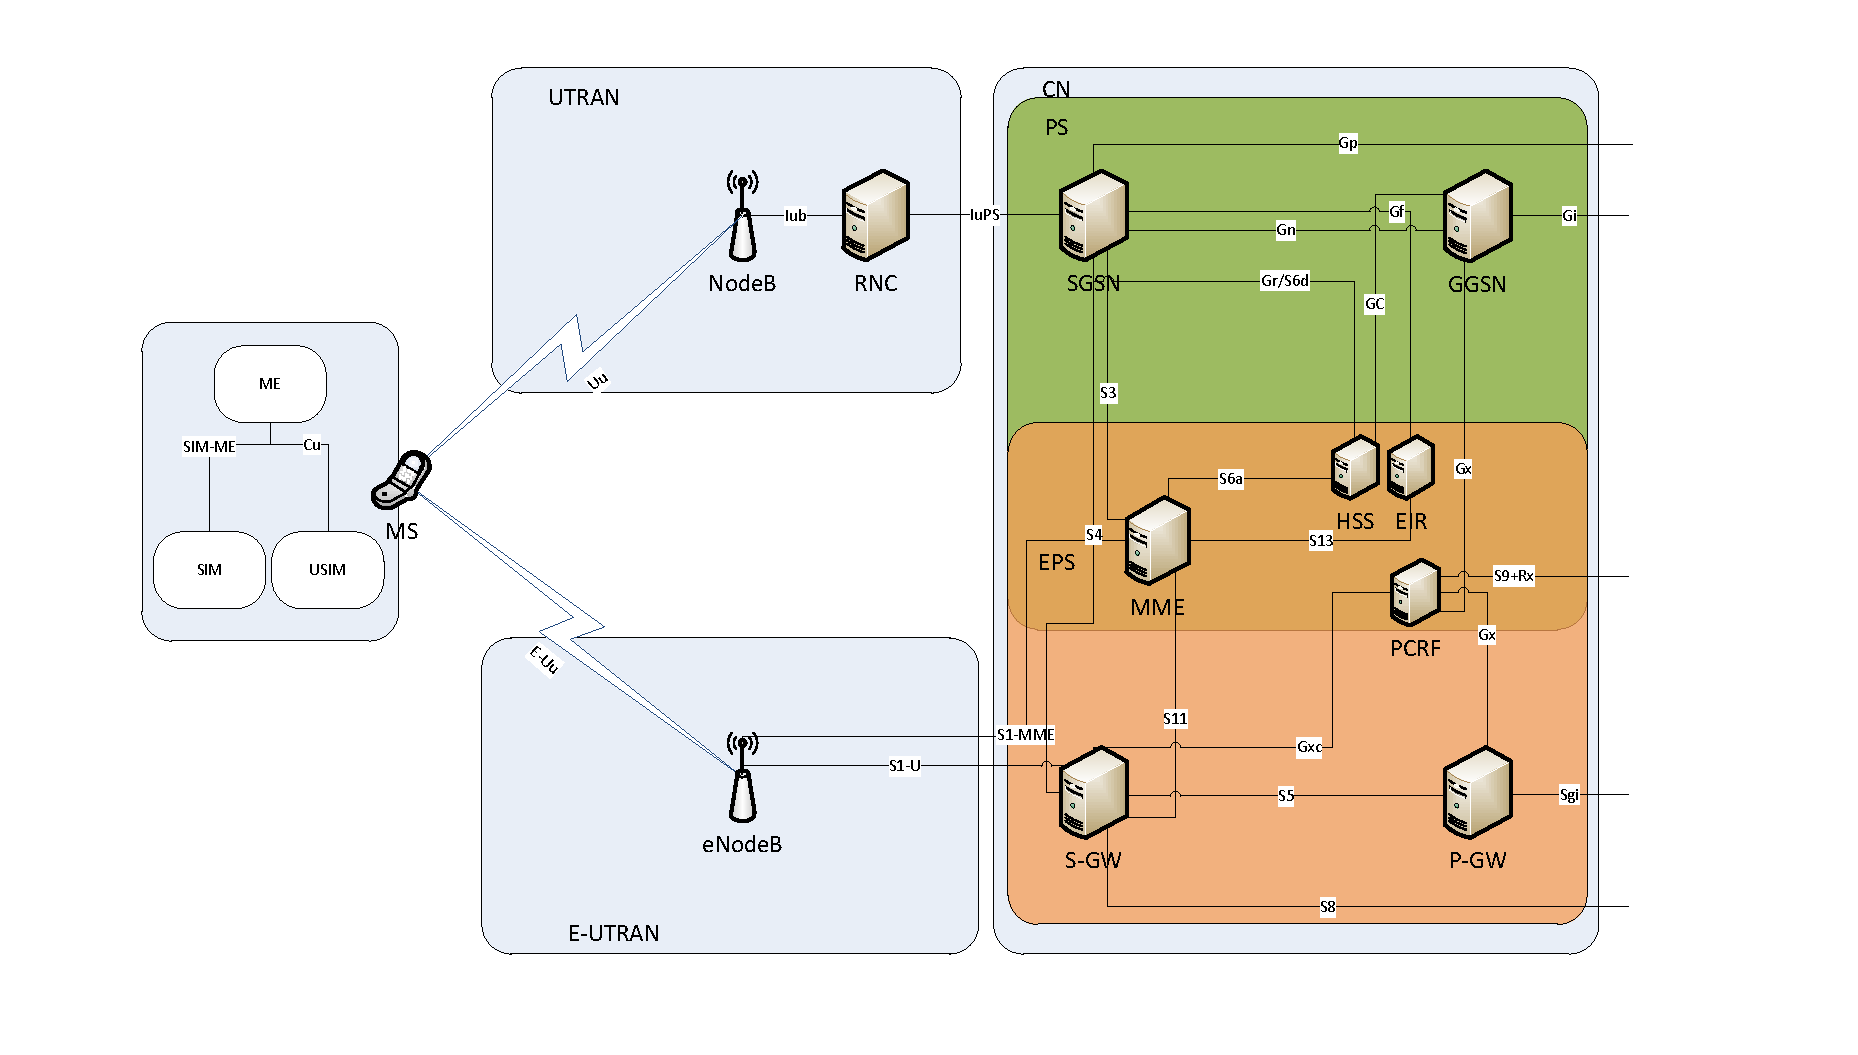
\includegraphics[width=1.0\textwidth]{images/3gpp/eps_ps-overview.pdf}
 \caption{Beispielnetz}\label{fig:netzwerk2}
\end{figure}

List of interfaces in the 3G/LTE PS network
\begin{itemize}
\item \textbf{Uu}: Interface between the mobile station (MS) and the fixed network part in Iu mode. The Uu interface is the Iu mode network interface for providing packet data services over the radio to the MS. The MT part of the MS is used to access the UMTS services through this interface.
\item \textbf{Iub}: Interface between a NodeB and a RNC.
\item \textbf{IuPS}: Interface between a RNC and a SGSN.

\item \textbf{S1-U}: Interface between a eNodeB and a S-GW. User plane bearer tunneling.
\item \textbf{S1-MME}: Interface between a eNodeB and a MME.
\item \textbf{S3}: Interface between a SGSN and a MME. User/bearer information exchange for active/idle state 3g network access mobility.
\item \textbf{S4}: Interface between a SGSN and a S-GW.	 2G user plane tunneling. GPRS mobility and control.
\item \textbf{S5}: Interface between a S-GW and a P-GW within the same PLMN. User plane tunneling; S-GW relocation due to mobility.
\item \textbf{S6a}: Interface between a MME and a HSS. Auth/auth data transfer to evolved system.
\item \textbf{Gr/S6d}: Interface between a SGSN and a HSS. 
\item \textbf{S8}: Interface between a S-GW and a P-GW in different PLMNs. Inter-PLMN variant to S5.
\item \textbf{S9}: Interface between a PRCF and the packet data network. Data exchange to visited PCRF PLMN.
\item \textbf{S11}: Interface between a S-GW and a MME.
\item \textbf{S12}: UTRAN to S-GW reference point. Based on Iu-u/Gn-u. Direct Tunnel via GTP-U.
\item \textbf{S13}: Interface between a MME and a EIR. UE identity check.
\item \textbf{SGi}: The reference point between the EPC based PLMN and the packet data network. Same as Gi for 3gpp.

\item \textbf{GC}: Interface between a HSS and a GGSN.
\item \textbf{Gf}: Interface between a SGSN and a EIR.
\item \textbf{Gi}: Reference point between Packet Domain and an external packet data network.
\item \textbf{Gn}: Interface between two GSNs within the same PLMN.
\item \textbf{Gp}: Interface between two GSNs in different PLMNs. The Gp interface allows support of Packet Domain network services across areas served by the co-operating PLMNs.
\item \textbf{Gx}: Interface between a PCRF and a P-GW/GGSN. QoS policy and charging rules transfer.
\item \textbf{Gxc}: Interface between a PCRF and a S-GW.

\item \textbf{Rx}: Interface between a PRCF and the packet data network.
\end{itemize}

\section{Control Plane Protocol Stacks}

\begin{figure}[htbp]
 \centering
 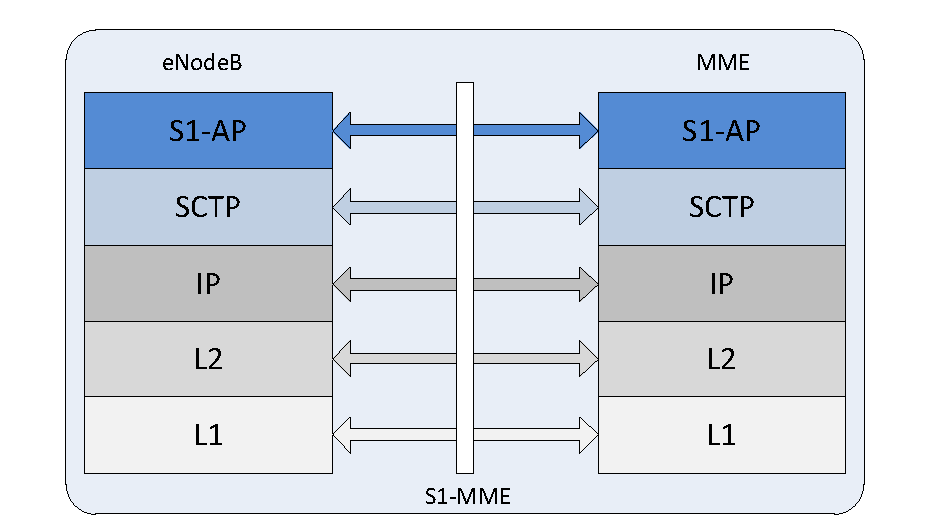
\includegraphics[width=1.0\textwidth]{images/3gpp/eNB-MME-layers.pdf}
 \caption{Beispielnetz}\label{fig:3gpp-enbmme}
\end{figure}

\begin{figure}[htbp]
 \centering
 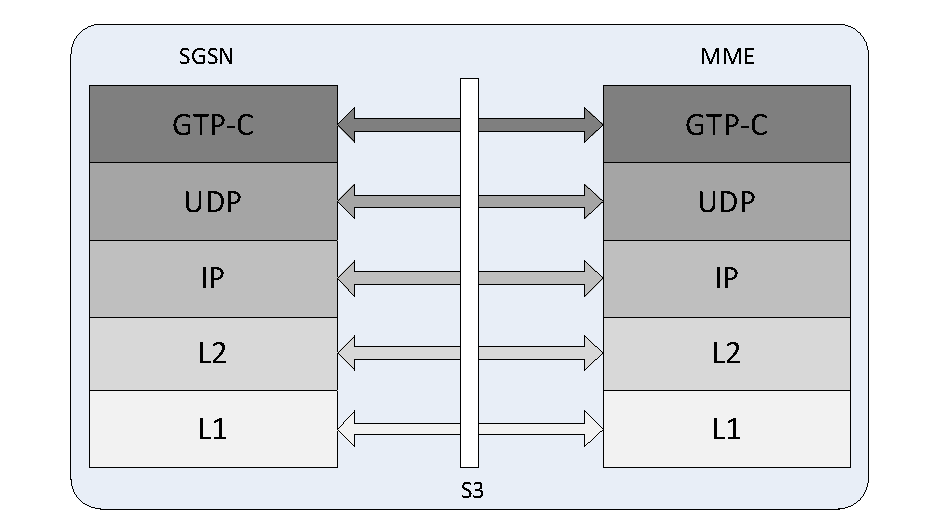
\includegraphics[width=1.0\textwidth]{images/3gpp/SGSN-MME-layers.pdf}
 \caption{Beispielnetz}\label{fig:3gpp-sgsnmme}
\end{figure}

\begin{figure}[htbp]
 \centering
 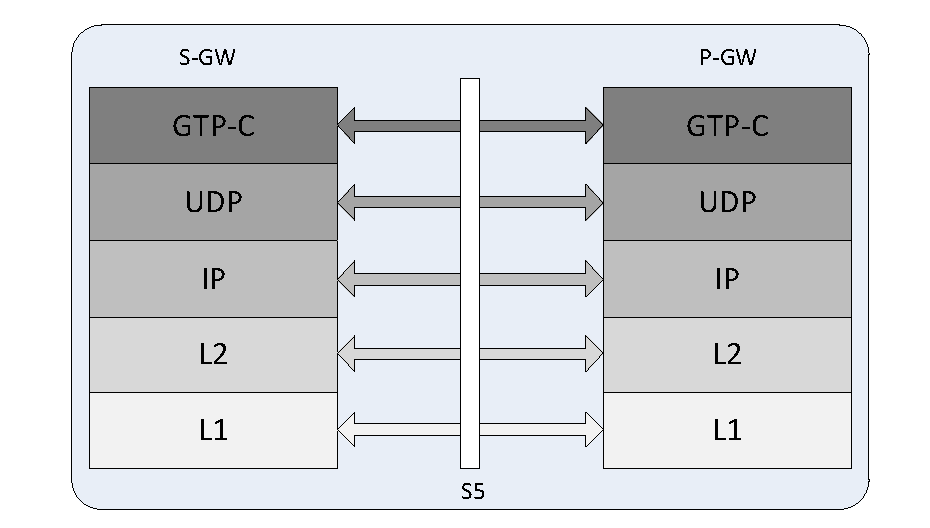
\includegraphics[width=1.0\textwidth]{images/3gpp/S-GW-P-GW-layers.pdf}
 \caption{Beispielnetz}\label{fig:3gpp-sgwpgw}
\end{figure}

\begin{figure}[htbp]
 \centering
 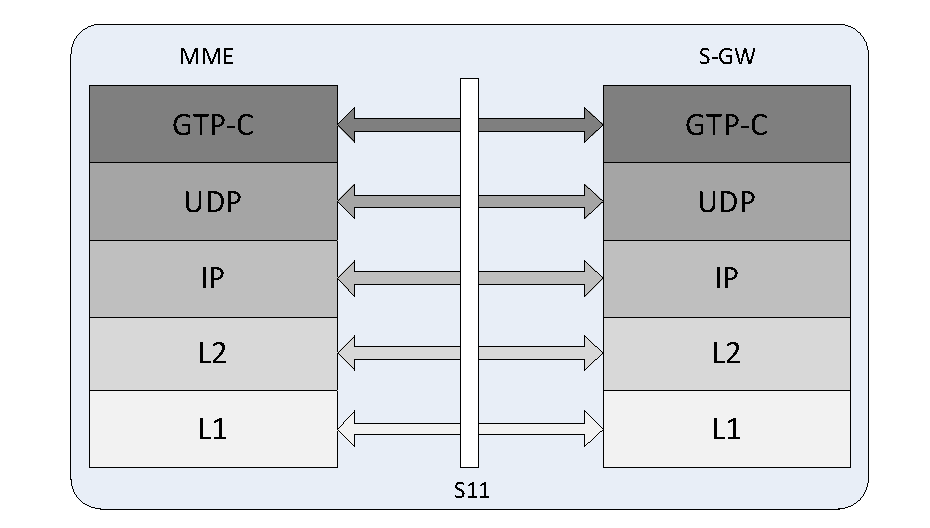
\includegraphics[width=1.0\textwidth]{images/3gpp/MME-S-GW-layers.pdf}
 \caption{Beispielnetz}\label{fig:3gpp-mmesgw}
\end{figure}


\begin{figure}[htbp]
 \centering
 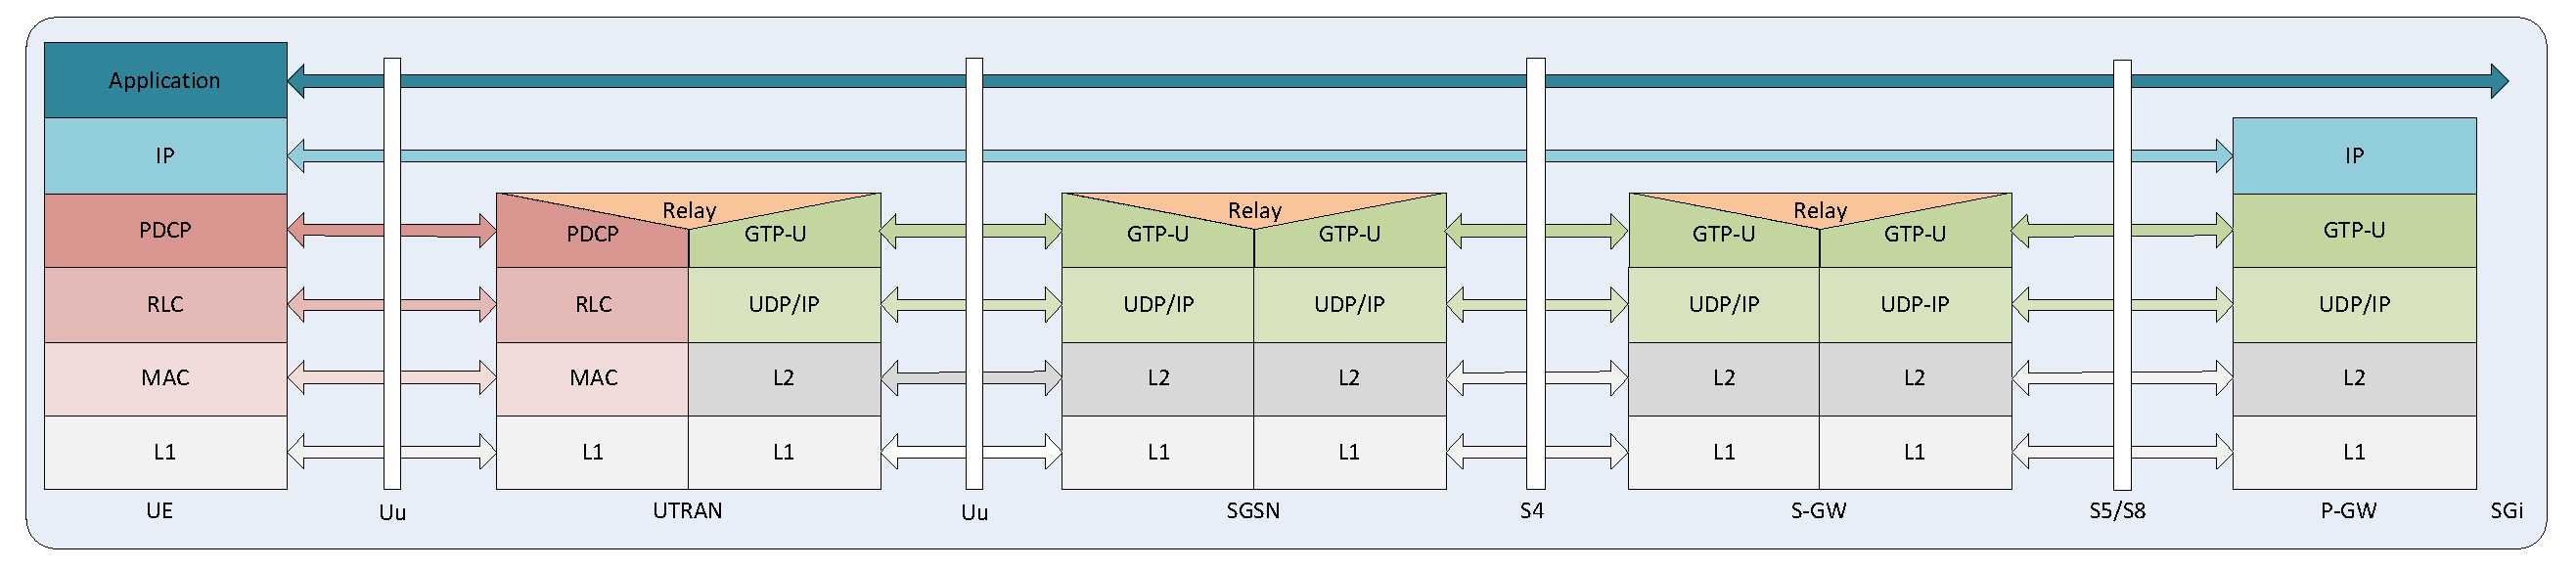
\includegraphics[width=1.0\textwidth]{images/3gpp/3g-userplane.pdf}
 \caption{Beispielnetz}\label{fig:3gpp-umtsuserplane}
\end{figure}

\begin{figure}[htbp]
 \centering
 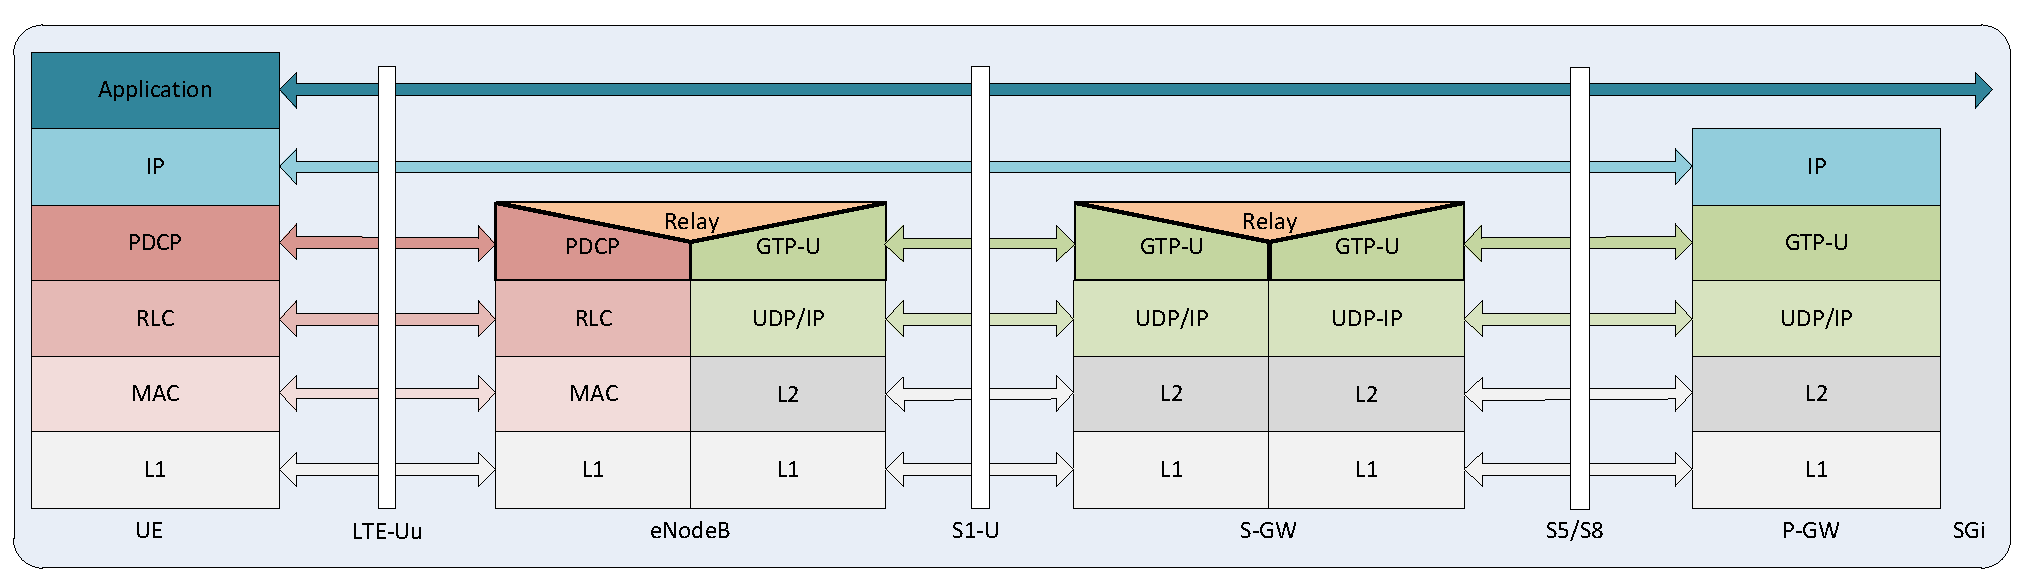
\includegraphics[width=1.0\textwidth]{images/3gpp/LTE-userplane.pdf}
 \caption{Beispielnetz}\label{fig:3gpp-lteuserplane}
\end{figure}


\section{Bearers}

As you said only 11 bearer are permitted.
So PDN connection(Default bearer) + Dedicated bearers put together should not exceed 11 bearers at any instant of time at UE side.
Theoretically 11 PDN connections are possible. But i dont think it will be of any use in practical EPS topology.

One UE Can have Maximum 3 PDN connection.
where as my knowledge is concern one UE can support maximum 11 bearers, 3 default and 8 dedicated bearers.

Does I will get in any spec for this. As the default bearer are of  NON-GBR type and and there are 5-9 are of NON-GBR QCI so I think a ue can have maximum 5 default bearer If two default bearer can not use same QCI.

\begin{figure}[htbp]
 \centering
 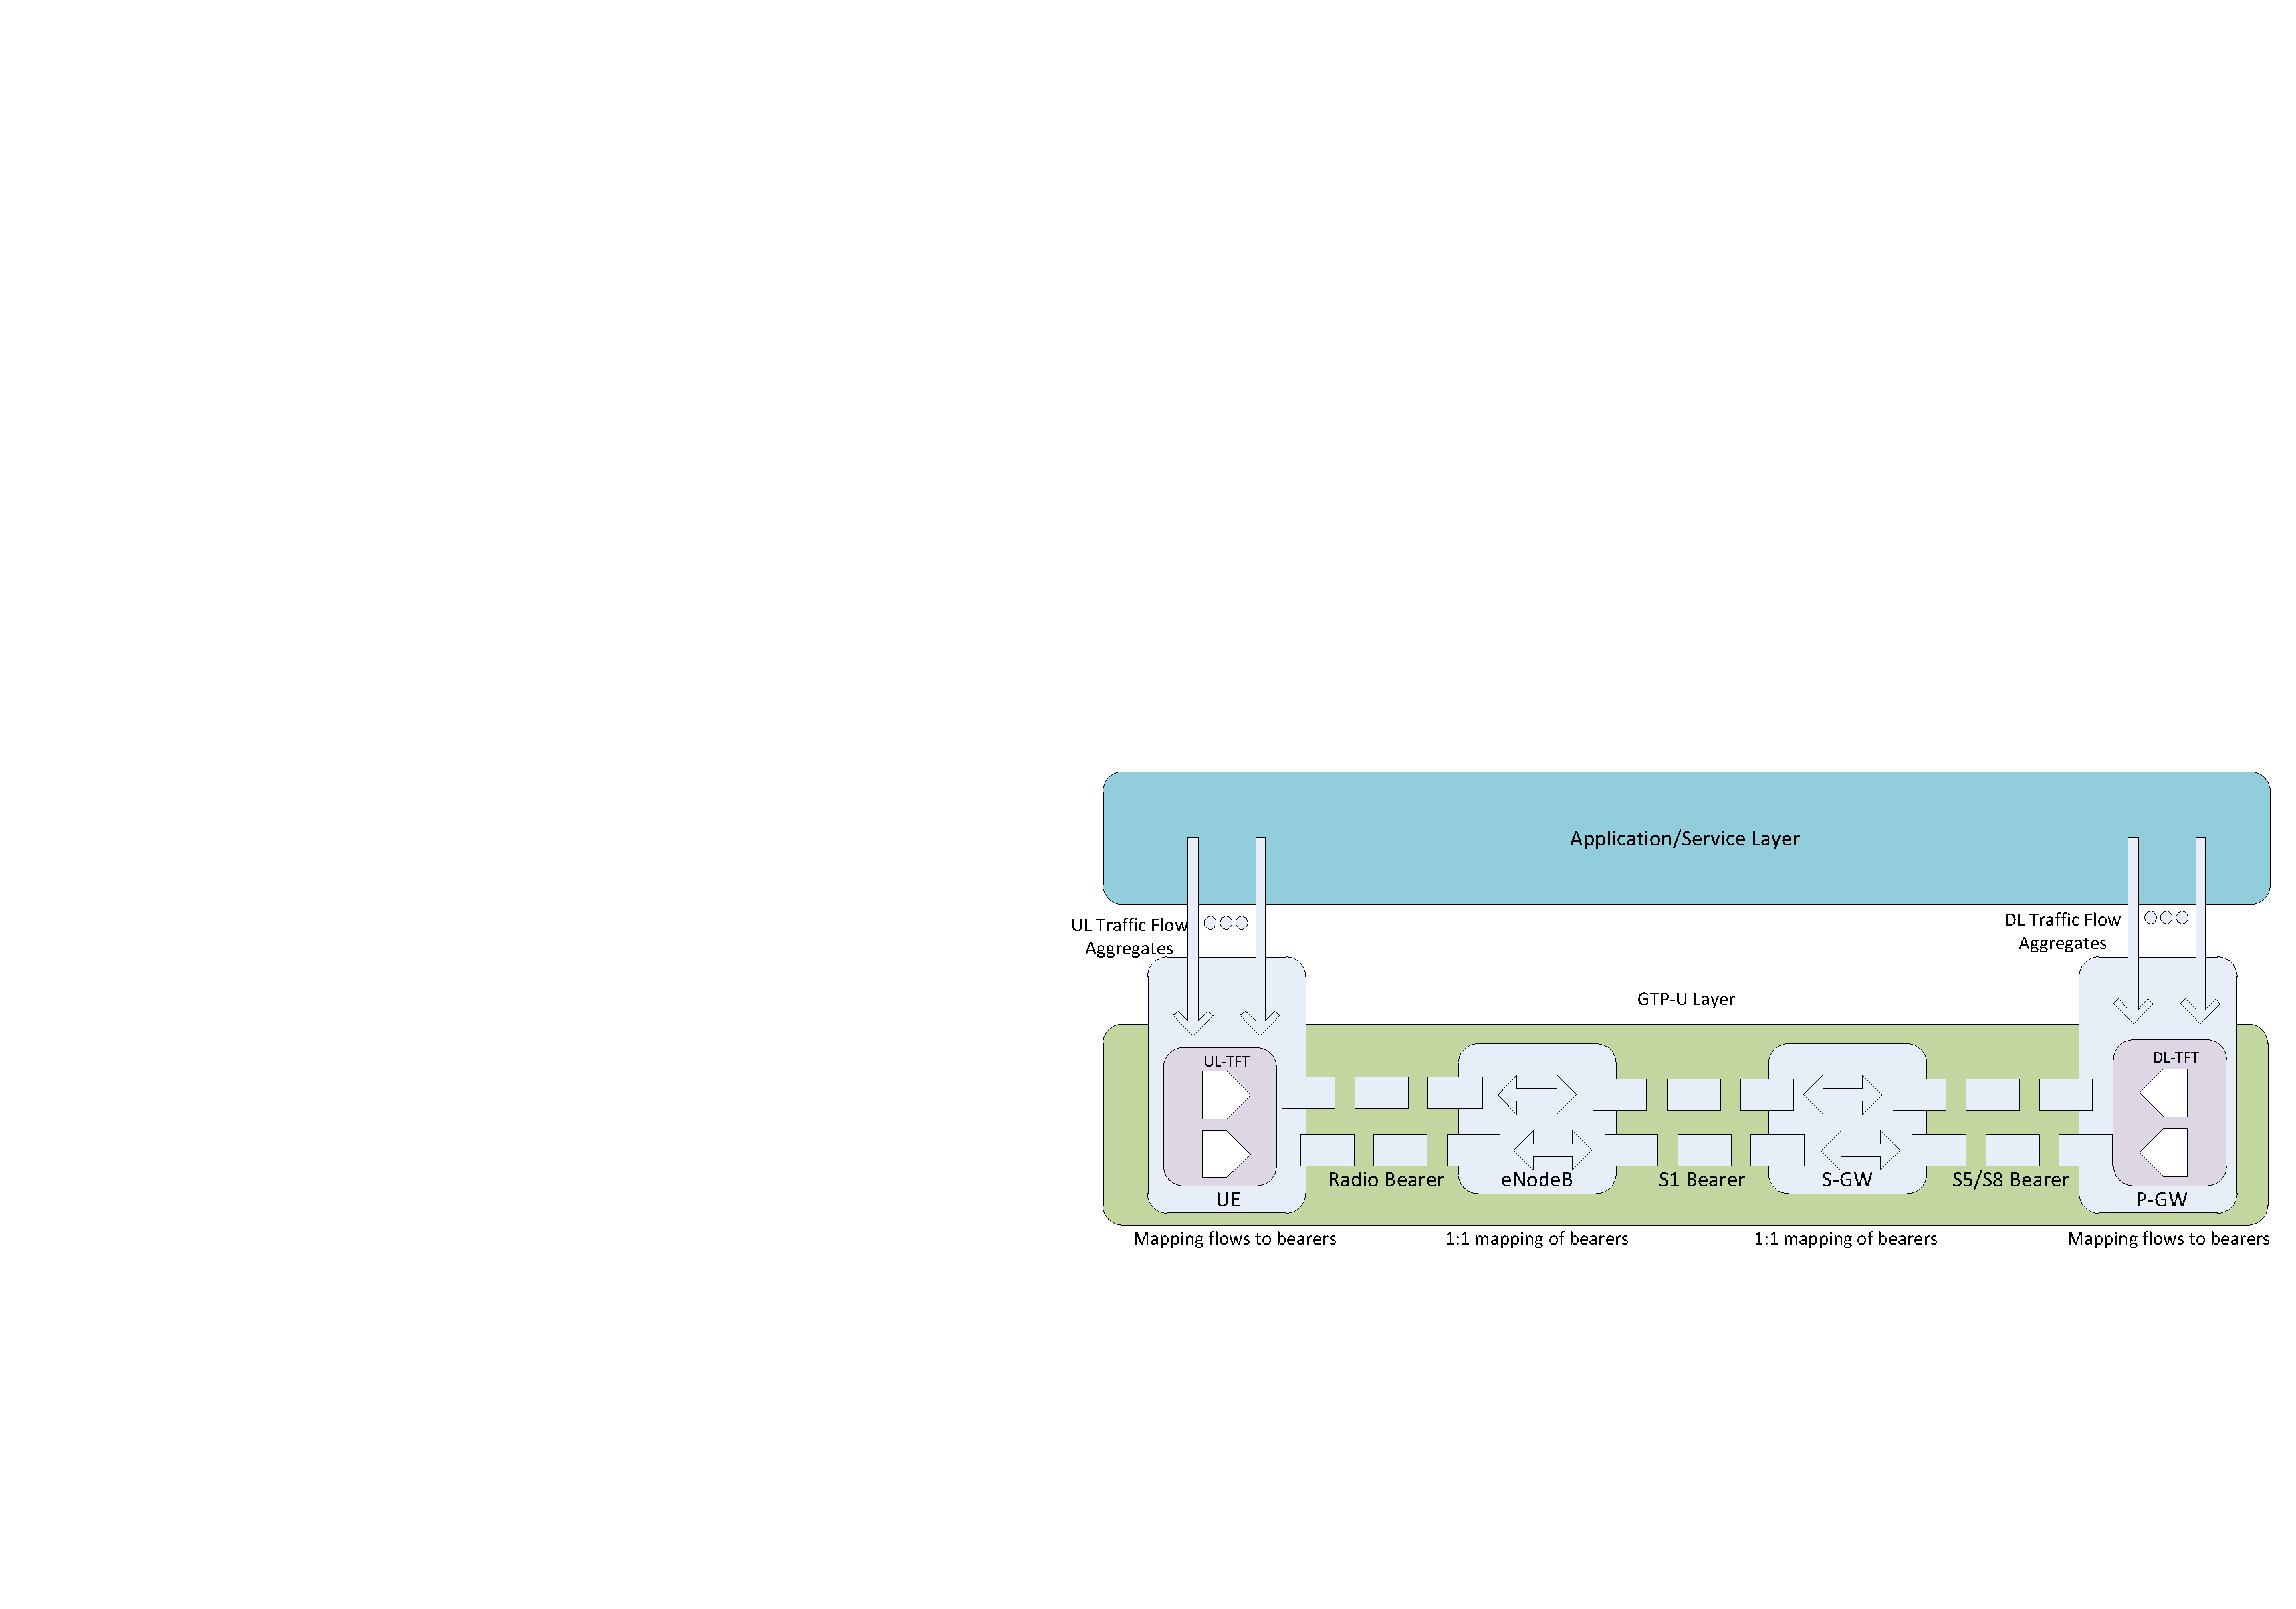
\includegraphics[width=1.0\textwidth]{images/3gpp/bearers.pdf}
 \caption{Beispielnetz}\label{fig:3gpp-bearers}
\end{figure}


\begin{figure}[htbp]
 \centering
 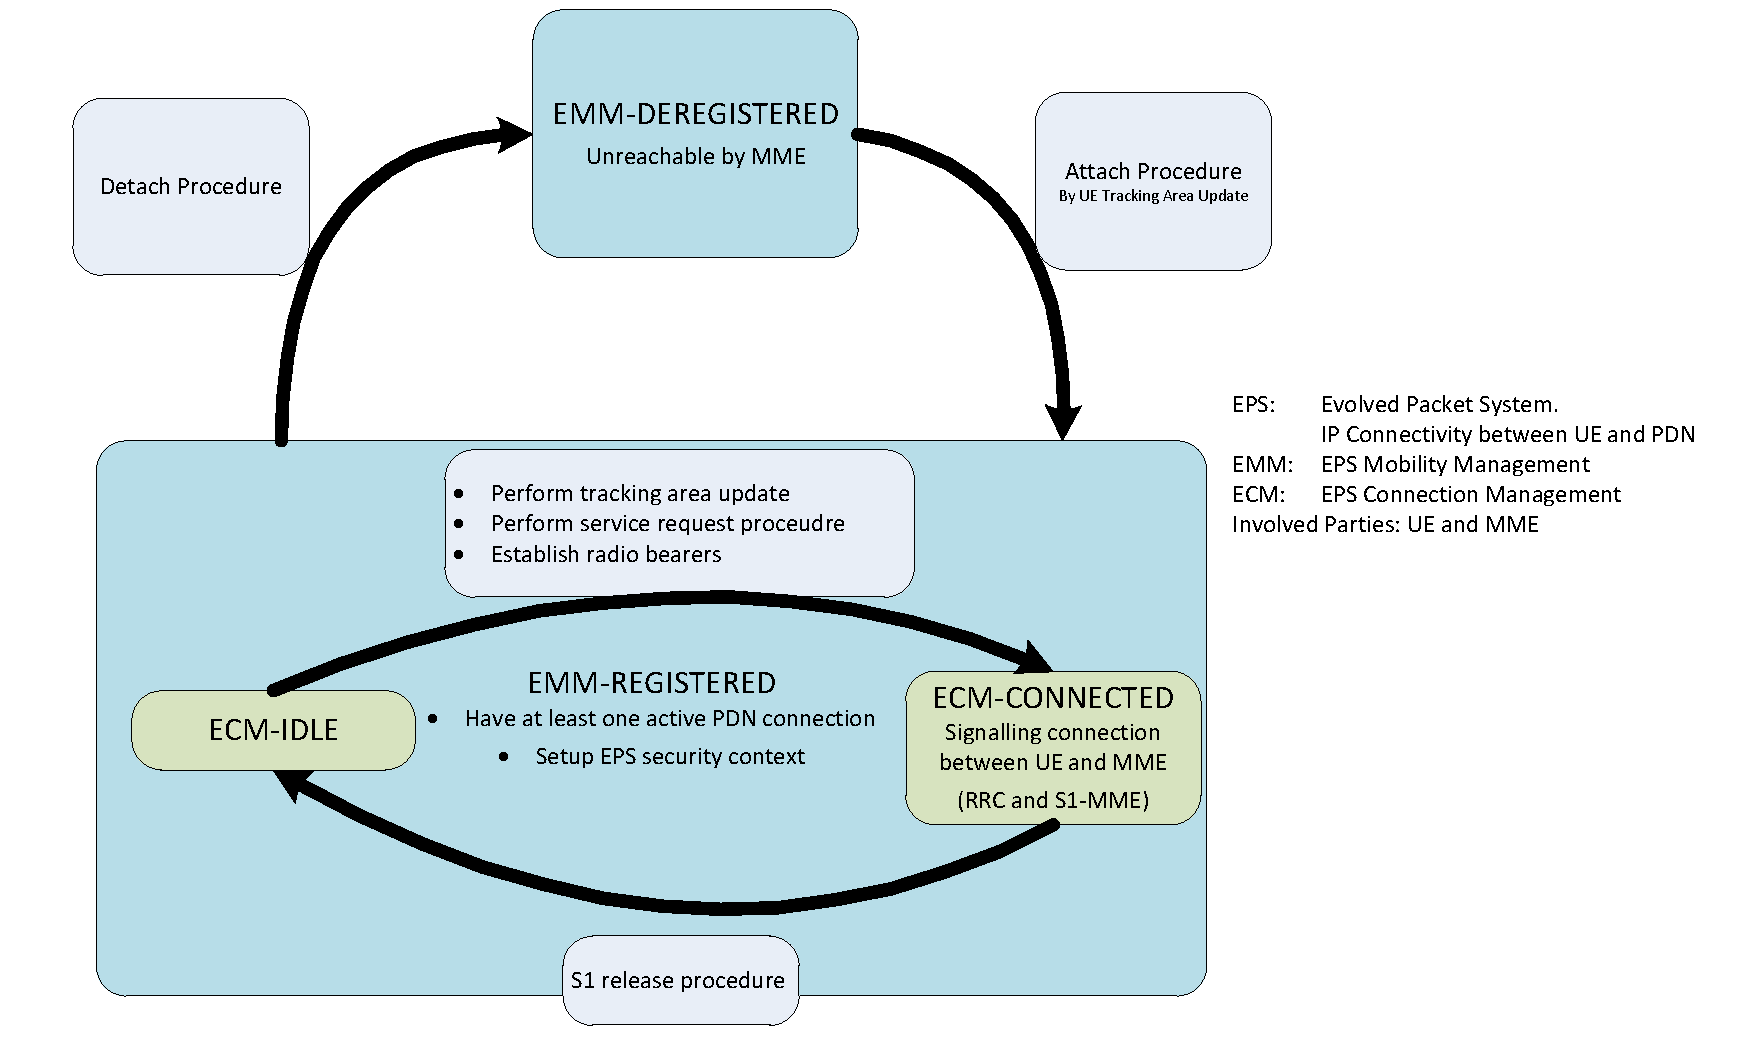
\includegraphics[width=1.0\textwidth]{images/3gpp/ECM-states.pdf}
 \caption{Beispielnetz}\label{fig:3gpp-ecmstates}
\end{figure}

\begin{itemize}
\item 	Every bearer has a predefined QoS level between UE and P-GW.
		==> Level of Granularity for QoS control.
\item	Initial bearer QoS level assigned by network based on subscription data.
\item	Guaranteed Bit Rate (GBR) bearers: dedicated network resources permanently allocated at est/mod. Otherwise Non-GBR.
\item	The Traffic Flow Template (TFT) belonging to a bearer is a set of packet filters that assign traffic flows to the bearer.
\item	UL-TFT at UE, DL-TFT at PCEF (P-GW).
\item 	default bearer: always-on IP connectivity for the UE to a PDN
\item	dedicated bearer:   
			\begin{itemize}
				\item any additional bearer for the same PDN
				\item Traffic Flow Template (TFT) associated with every ded. bearer
				\item establishment/modification decision only by EPC
				\item QoS level assignment only by EPC
			\end{itemize}

\item	default bearer may be used as {m,c}atch-all traffic bearer for everything that does not match any filter
\item	Every bearer associated with QCI and ARP.

QoS class identifier (QCI): standardized scalar as reference for node-specific QoS parameters
Allocation and Retention Policy (ARP): priority level preemption capability, preemption vulnerability.

\item	All simultaneously active bearers by one UE are provided are provided by the same P-GW.
\end{itemize}

EMM Service request procedure

\begin{figure}[htbp]
 \centering
 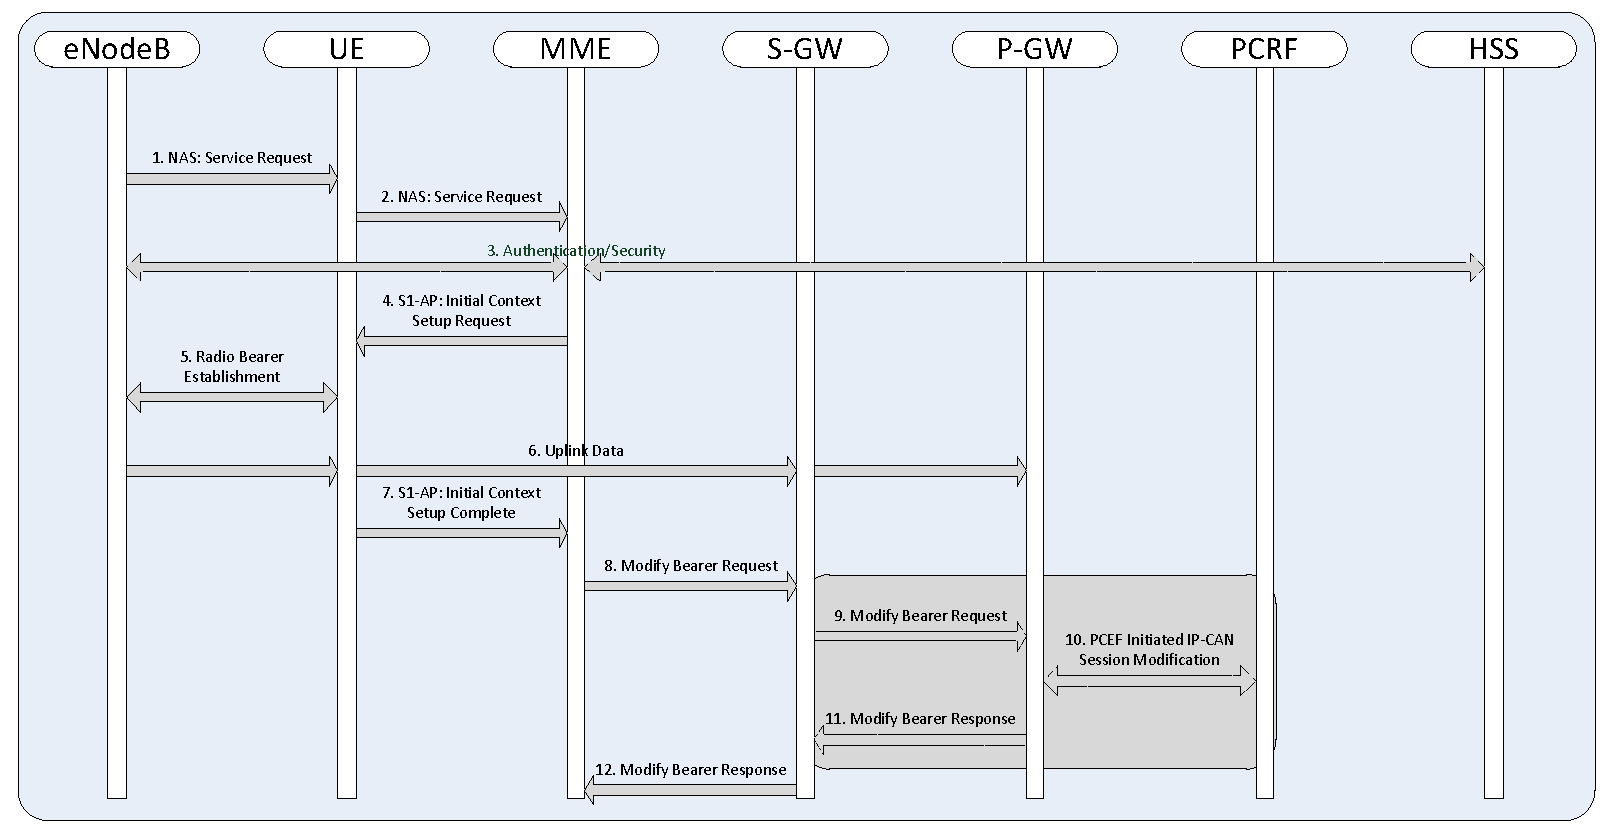
\includegraphics[width=1.0\textwidth]{images/3gpp/UE-service-request.pdf}
 \caption{Beispielnetz}\label{fig:3gpp-ueservicereq}
\end{figure}

Annotations:
1. Encapsulated in RRC message.
2. Forwarded in S1-AP Initial UE Message.
3. Various security procedures.


\section{Information Storage}
per PLMN node, cf. 3GPP TS 23.401 clause 5.7.

\begin{figure}[htbp]
 \centering
 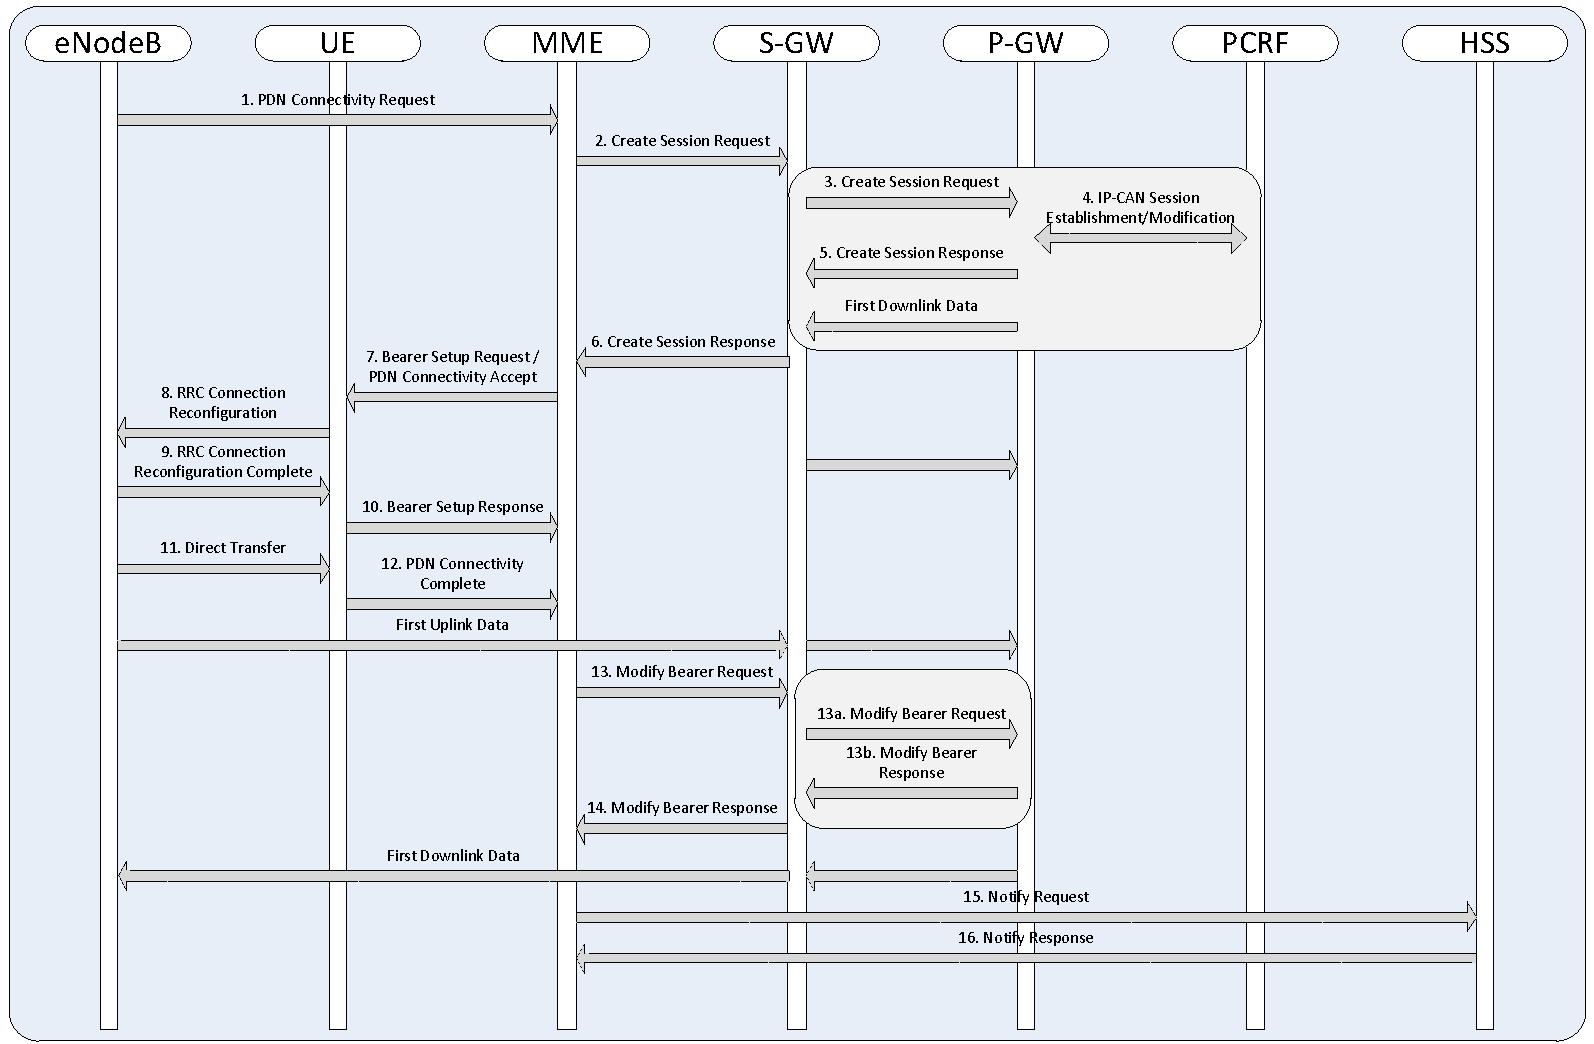
\includegraphics[width=1.0\textwidth]{images/3gpp/UE-requested-PDN-connectivity.pdf}
 \caption{Beispielnetz}\label{fig:3gpp-uepdnreq}
\end{figure}


\section{GTP}
\subsection{GTPv2}



\begin{tabular}{c|c|c|c|c|c|c|c|c|}
\multicolumn{1}{c}{} & \multicolumn{8}{c}{\textbf{Bits}} \\
\cline{2-9} \textbf{Octets} & 8 & 7 & 6 & 5 & 4 & 3 & 2 & 1 \\ 
\cline{2-9} 1 & \multicolumn{3}{c|}{Version}  & P & T & Spare & Spare & Spare \\ 
\cline{2-9} 2 & \multicolumn{8}{c|}{Message Type}  \\ 
\cline{2-9} 3 & \multicolumn{8}{c|}{Message Length (1st Octet)}  \\ 
\cline{2-9} 4 & \multicolumn{8}{c|}{Message Length (2nd Octet)}  \\ 
\cline{2-9} m to & \multicolumn{8}{c|}{\multirow{2}{10cm}{If T flag is set to 1, then TEID shall be placed into octets 5-8. Otherwise, TEID field is not present at all.}} \\ 
 k(m+3) & \multicolumn{8}{c|}{} \\ 
\cline{2-9} n to (n+2) & \multicolumn{8}{c|}{Sequence Number} \\ 
\cline{2-9} (n+3) & \multicolumn{8}{c|}{Spare} \\ 
\cline{2-9} 
\end{tabular} 
\subsection{GTP-C}

\begin{tabular}{c|c|c|c|c|c|c|c|c|}
\multicolumn{1}{c}{} & \multicolumn{8}{c}{\textbf{Bits}} \\
\cline{2-9} \textbf{Octets} & 8 & 7 & 6 & 5 & 4 & 3 & 2 & 1 \\ 
\cline{2-9} 1 & \multicolumn{3}{c|}{Version}  & P & T=1 & Spare & Spare & Spare \\ 
\cline{2-9} 2 & \multicolumn{8}{c|}{Message Type}  \\ 
\cline{2-9} 3 & \multicolumn{8}{c|}{Message Length (1st Octet)}  \\ 
\cline{2-9} 4 & \multicolumn{8}{c|}{Message Length (2nd Octet)}  \\ 
\cline{2-9} 5 & \multicolumn{8}{c|}{Tunnel Endpoint Identifier (1st Octet)} \\ 
\cline{2-9} 6 & \multicolumn{8}{c|}{Tunnel Endpoint Identifier (2nd Octet)} \\ 
\cline{2-9} 7 & \multicolumn{8}{c|}{Tunnel Endpoint Identifier (3rd Octet)} \\ 
\cline{2-9} 8 & \multicolumn{8}{c|}{Tunnel Endpoint Identifier (4th Octet)} \\ 
\cline{2-9} 9 & \multicolumn{8}{c|}{Sequence Number (1st Octet)} \\
\cline{2-9} 10 & \multicolumn{8}{c|}{Sequence Number (2nd Octet)} \\
\cline{2-9} 11 & \multicolumn{8}{c|}{Sequence Number (3rd Octet)} \\
\cline{2-9} 12 & \multicolumn{8}{c|}{Spare} \\
\cline{2-9}
\end{tabular} 

12 Byte GTPv2-C header.

\subsubsection{Create Session Request Message}

Information Elements Table for PDP Context Activation Case only

\begin{longtabu}{|p{2cm}|c|p{1.5cm}|p{8cm}|}
\hline
Information Element 						& IE Type 					& Max Wire Size (Bytes)	& Comment \\ \hline
IMSI 										& IMSI 						& 12					& \\ \hline
MSISDN 										& MSISDN					& 12					& On S11 Interface if provided by HSS; In case of UE requested connectivity if MME has it stored. \\ \hline
MEI Identity 								& MEI 						& 12					& If available at MME. \\ \hline
User Location Information 					& ULI						& 						& E-UTRAN initial attach \&  UE requested connectivity only; included by S-GW if received from MME via S5/S8; included on S4 and S5/S8 for PDP context activation, either CGI, SAI, or RAI. \\ \hline
Serving Network								& Serving Network			& 						& Initial E-UTRAN attach, context activation and UE requested connectivity \\ \hline
RAT Type									& RAT Type					& 5						& \\ \hline
Indication Flags							& Indication				& 6						& Flags: S5/S8 Protocol Type; Dual Address Bearer Flag; Handover Indication; Direct Tunnel Flag; Piggybacking Supported; Change Reporting Support Indication \\ \hline
Sender F-TEID for Control Plane				& F-TEID					& 						& \\ \hline
P-G S5/S8 Address for Control Plane or PMIP	& F-TEID					& 						& On S11/S4 interfaces; 0 if initial attach, context activation or PDN connectivity \\ \hline
Access Point Name							& APN						& 83					& \\ \hline
Selection Mode								& Selection Mode			& 						& Indicate whether subscribed or non-subscribed, chosen by MME, was selected \\ \hline
PDN Type									& PDN Type					& 						& IPv4, IPv6 or IPv4v6. \\ \hline
PDN Address Allocation						& PAA						& 26					& Set to static IP address; else (dynamic) to 0.0.0.0 or IPv6 Prefix Length 0. \\ \hline
Maximum APN Restriction						& APN Restriction			& 						& Set to most stringent restriction of any active bearer. \\ \hline
Aggregate Maximum Bit Rate					& ABMR						& 12					& \\ \hline
Protocol Configuration Options				& PCO						& 254					& Forwarded from UE to P-GW via S-GW via MME. \\ \hline
Bearer Contexts to be created				& Bearer Context			& 						& present multiple times to represent list of bearers \\ \hline
Trace Information							& Trace Information 		& 						& If S-GW / P-GW is activated. \\ \hline
Recovery									& Recovery					& 5						& If peer node contacted for the first time. \\ \hline
MME-FQ-CSID									& FQ-CSID					& 						& Included by MME on S11 \\ \hline
SGW-FQ-CSID									& FQ-CSID					& 						& Included by S-GW on S5/S8 \\ \hline
UE Time Zone								& UE Time Zone 				& 						& Can be included by MME on S11; forwarded to P-GW via S-GW \\ \hline
User CSG Information						& UCI						& 						& If UE accessed via CSG cell or hybrid cell \\ \hline
Charging Characteristics					& Charging Characteristics	&						& \\ \hline
Private Extensions							& Private Extensions		&						& \\ \hline

\end{longtabu}

\subsubsection{Information Elements Wire Format}

\paragraph{IMSI}

\begin{tabular}{c|p{1cm}|p{1cm}|p{1cm}|p{1cm}|p{1cm}|p{1cm}|p{1cm}|p{1cm}|}
\multicolumn{1}{c}{} & \multicolumn{8}{c}{\textbf{Bits}} \\
\cline{2-9} \textbf{Octets} & 8 & 7 & 6 & 5 & 4 & 3 & 2 & 1 \\ 
\cline{2-9} 1 & \multicolumn{8}{c|}{Type = 1 (decimal)} \\ 
\cline{2-9} 2 to 3 & \multicolumn{8}{c|}{Length = n}  \\ 
\cline{2-9} 4 & \multicolumn{4}{c|}{Spare} & \multicolumn{4}{c|}{Instance} \\ 
\cline{2-9} 5 & \multicolumn{4}{c|}{Number digit 2} & \multicolumn{4}{c|}{Number digit 1} \\ 
\cline{2-9} 6 & \multicolumn{4}{c|}{Number digit 4} & \multicolumn{4}{c|}{Number digit 3} \\ 
\cline{2-9} ... & \multicolumn{4}{c|}{...} & \multicolumn{4}{c|}{...} \\ 
\cline{2-9} n+4 & \multicolumn{4}{c|}{Number digit m} & \multicolumn{4}{c|}{Number digit m-1} \\ 
\cline{2-9}
\end{tabular} 

Decimals coded as TBCD; if odd number fill last nibble with 1; max digits is 15.\\
Max IE size 12 Byte.

\paragraph{APN}

\begin{tabular}{c|p{1cm}|p{1cm}|p{1cm}|p{1cm}|p{1cm}|p{1cm}|p{1cm}|p{1cm}|}
\multicolumn{1}{c}{} & \multicolumn{8}{c}{\textbf{Bits}} \\
\cline{2-9} \textbf{Octets} & 8 & 7 & 6 & 5 & 4 & 3 & 2 & 1 \\ 
\cline{2-9} 1 & \multicolumn{8}{c|}{Type = 71 (decimal)} \\ 
\cline{2-9} 2 to 3 & \multicolumn{8}{c|}{Length = n}  \\ 
\cline{2-9} 4 & \multicolumn{4}{c|}{Spare} & \multicolumn{4}{c|}{Instance} \\ 
\cline{2-9} 5 to (n+4) & \multicolumn{8}{c|}{Access Point Name} \\ 
\cline{2-9}
\end{tabular} 

Full APN name including APN Network Identifier and APN Operator Identifier.
Network Identifier: max length 63 bytes.
Operator Identifier: mnc<3digits>.mcc<3digits>.gprs; 16 bytes (18 incl dots).
(Ex: ggsn-cluster-A.provinceB.mnc012.mcc345.gprs)

Max total $4+63+16=83$

\paragraph{AMBR}

\begin{tabular}{c|p{1cm}|p{1cm}|p{1cm}|p{1cm}|p{1cm}|p{1cm}|p{1cm}|p{1cm}|}
\multicolumn{1}{c}{} & \multicolumn{8}{c}{\textbf{Bits}} \\
\cline{2-9} \textbf{Octets} & 8 & 7 & 6 & 5 & 4 & 3 & 2 & 1 \\ 
\cline{2-9} 1 & \multicolumn{8}{c|}{Type = 72 (decimal)} \\ 
\cline{2-9} 2 to 3 & \multicolumn{8}{c|}{Length = n}  \\ 
\cline{2-9} 4 & \multicolumn{4}{c|}{Spare} & \multicolumn{4}{c|}{Instance} \\ 
\cline{2-9} 5 to 8 & \multicolumn{8}{c|}{APN-AMBR for uplink} \\ 
\cline{2-9} 9 to 12 & \multicolumn{8}{c|}{APN-AMBR for downlink} \\ 
\cline{2-9}
\end{tabular} 


Total size 12 bytes.


\paragraph{Recovery}

\begin{tabular}{c|p{1cm}|p{1cm}|p{1cm}|p{1cm}|p{1cm}|p{1cm}|p{1cm}|p{1cm}|}
\multicolumn{1}{c}{} & \multicolumn{8}{c}{\textbf{Bits}} \\
\cline{2-9} \textbf{Octets} & 8 & 7 & 6 & 5 & 4 & 3 & 2 & 1 \\ 
\cline{2-9} 1 & \multicolumn{8}{c|}{Type = 3 (decimal)} \\ 
\cline{2-9} 2 to 3 & \multicolumn{8}{c|}{Length = n}  \\ 
\cline{2-9} 4 & \multicolumn{4}{c|}{Spare} & \multicolumn{4}{c|}{Instance} \\ 
\cline{2-9} 5 to (n+4) & \multicolumn{8}{c|}{Recovery (Restart Counter} \\ 
\cline{2-9}
\end{tabular} 

IN GTPv2 first release IE length is 5 bytes. May be longer in the future.


\paragraph{MEI}

\begin{tabular}{c|p{1cm}|p{1cm}|p{1cm}|p{1cm}|p{1cm}|p{1cm}|p{1cm}|p{1cm}|}
\multicolumn{1}{c}{} & \multicolumn{8}{c}{\textbf{Bits}} \\
\cline{2-9} \textbf{Octets} & 8 & 7 & 6 & 5 & 4 & 3 & 2 & 1 \\ 
\cline{2-9} 1 & \multicolumn{8}{c|}{Type = 75 (decimal)} \\ 
\cline{2-9} 2 to 3 & \multicolumn{8}{c|}{Length = n}  \\ 
\cline{2-9} 4 & \multicolumn{4}{c|}{Spare} & \multicolumn{4}{c|}{Instance} \\ 
\cline{2-9} 5 to (n+4) & \multicolumn{8}{c|}{Mobile Equipment (ME) Identity} \\ 
\cline{2-9}
\end{tabular} 

15 (IMEI) or 16 (IMEISV) BCD digits filled with 1 to full octet. Size is 12 bytes.

\paragraph{MSISDN}

\begin{tabular}{c|p{1cm}|p{1cm}|p{1cm}|p{1cm}|p{1cm}|p{1cm}|p{1cm}|p{1cm}|}
\multicolumn{1}{c}{} & \multicolumn{8}{c}{\textbf{Bits}} \\
\cline{2-9} \textbf{Octets} & 8 & 7 & 6 & 5 & 4 & 3 & 2 & 1 \\ 
\cline{2-9} 1 & \multicolumn{8}{c|}{Type = 76 (decimal)} \\ 
\cline{2-9} 2 to 3 & \multicolumn{8}{c|}{Length = n}  \\ 
\cline{2-9} 4 & \multicolumn{4}{c|}{Spare} & \multicolumn{4}{c|}{Instance} \\ 
\cline{2-9} 5 & \multicolumn{4}{c|}{Number digit 2} & \multicolumn{4}{c|}{Number digit 1} \\ 
\cline{2-9} 6 & \multicolumn{4}{c|}{Number digit 4} & \multicolumn{4}{c|}{Number digit 3} \\ 
\cline{2-9} ... & \multicolumn{4}{c|}{...} & \multicolumn{4}{c|}{...} \\ 
\cline{2-9} n+4 & \multicolumn{4}{c|}{Number digit m} & \multicolumn{4}{c|}{Number digit m-1} \\ 
\cline{2-9}
\end{tabular} 

MSISDN limited to 15 digits. Max total size 12 bytes.


\paragraph{Indication}
\centering
\begin{tabular}{c|p{1cm}|p{1cm}|p{1cm}|p{1cm}|p{1cm}|p{1cm}|p{1cm}|p{1cm}|}
\multicolumn{1}{c}{} & \multicolumn{8}{c}{\textbf{Bits}} \\
\cline{2-9} \textbf{Octets} & 8 & 7 & 6 & 5 & 4 & 3 & 2 & 1 \\ 
\cline{2-9} 1 & \multicolumn{8}{c|}{Type = 77 (decimal)} \\ 
\cline{2-9} 2 to 3 & \multicolumn{8}{c|}{Length = n}  \\ 
\cline{2-9} 4 & \multicolumn{4}{c|}{Spare} & \multicolumn{4}{c|}{Instance} \\ 
\cline{2-9} 5 & DAF & DTF & HI & DFI & OI & ISRSI & ISRAI & SGWCI \\ 
\cline{2-9} 6 & Spare & UIMSI & CFSI & CRSI & P & PT & SI & MSV \\ 
\cline{2-9} 7 to (n+4) & \multicolumn{8}{c|}{These octet(s) is/are present only if explicitly specified} \\ 
\cline{2-9}
\end{tabular} 

Size is 7 bytes.

\paragraph{PCO}
\centering
\begin{tabular}{c|p{1cm}|p{1cm}|p{1cm}|p{1cm}|p{1cm}|p{1cm}|p{1cm}|p{1cm}|}
\multicolumn{1}{c}{} & \multicolumn{8}{c}{\textbf{Bits}} \\
\cline{2-9} \textbf{Octets} & 8 & 7 & 6 & 5 & 4 & 3 & 2 & 1 \\ 
\cline{2-9} 1 & \multicolumn{8}{c|}{Type = 78 (decimal)} \\ 
\cline{2-9} 2 to 3 & \multicolumn{8}{c|}{Length = n}  \\ 
\cline{2-9} 4 & \multicolumn{4}{c|}{Spare} & \multicolumn{4}{c|}{Instance} \\ 
\cline{2-9} 5 to (n+4) & \multicolumn{8}{c|}{Protocol Configuration Options} \\
\cline{2-9}
\end{tabular} 

Minimum length 4+3-3, maximum length 4+253-3; average?


\paragraph{PAA}
\centering

\begin{tabular}{c|p{1cm}|p{1cm}|p{1cm}|p{1cm}|p{1cm}|p{1cm}|p{1cm}|p{1cm}|}
\multicolumn{1}{c}{} & \multicolumn{8}{c}{\textbf{Bits}} \\
\cline{2-9} \textbf{Octets} & 8 & 7 & 6 & 5 & 4 & 3 & 2 & 1 \\ 
\cline{2-9} 1 & \multicolumn{8}{c|}{Type = 79 (decimal)} \\ 
\cline{2-9} 2 to 3 & \multicolumn{8}{c|}{Length = n}  \\ 
\cline{2-9} 4 & \multicolumn{4}{c|}{Spare} & \multicolumn{4}{c|}{Instance} \\ 
\cline{2-9} 5 & \multicolumn{5}{c|}{Spare} & \multicolumn{3}{c|}{PDN Type} \\
\cline{2-9} 6 to (n+4) & \multicolumn{8}{c|}{PDN Adress and Prefix} \\
\cline{2-9}
\end{tabular} 

Either 9 (IPv4), 22 (IPv6), or 26 (IPv4v6).


\paragraph{RAT Type}
\centering
\begin{tabular}{c|p{1cm}|p{1cm}|p{1cm}|p{1cm}|p{1cm}|p{1cm}|p{1cm}|p{1cm}|}
\multicolumn{1}{c}{} & \multicolumn{8}{c}{\textbf{Bits}} \\
\cline{2-9} \textbf{Octets} & 8 & 7 & 6 & 5 & 4 & 3 & 2 & 1 \\ 
\cline{2-9} 1 & \multicolumn{8}{c|}{Type = 82 (decimal)} \\ 
\cline{2-9} 2 to 3 & \multicolumn{8}{c|}{Length = n}  \\ 
\cline{2-9} 4 & \multicolumn{4}{c|}{Spare} & \multicolumn{4}{c|}{Instance} \\ 
\cline{2-9} 5 & \multicolumn{8}{c|}{RAT Type} \\
\cline{2-9} 6 to (n+4) & \multicolumn{8}{c|}{These octet(s) is/are present only if explicitly specified} \\
\cline{2-9}
\end{tabular} 

Maximum length 5 to ?.

\paragraph{Serving Network}

\centering
\begin{tabular}{c|p{1cm}|p{1cm}|p{1cm}|p{1cm}|p{1cm}|p{1cm}|p{1cm}|p{1cm}|}
\multicolumn{1}{c}{} & \multicolumn{8}{c}{\textbf{Bits}} \\
\cline{2-9} \textbf{Octets} & 8 & 7 & 6 & 5 & 4 & 3 & 2 & 1 \\ 
\cline{2-9} 1 & \multicolumn{8}{c|}{Type = 83 (decimal)} \\ 
\cline{2-9} 2 to 3 & \multicolumn{8}{c|}{Length = n}  \\ 
\cline{2-9} 4 & \multicolumn{4}{c|}{Spare} & \multicolumn{4}{c|}{Instance} \\ 
\cline{2-9} 5 & \multicolumn{4}{c|}{MCC digit 2} & \multicolumn{4}{c|}{MCC digit 1} \\ 
\cline{2-9} 6 & \multicolumn{4}{c|}{MNC digit 3} & \multicolumn{4}{c|}{MCC digit 3} \\ 
\cline{2-9} 7 & \multicolumn{4}{c|}{MNC digit 2} & \multicolumn{4}{c|}{MNC digit 1} \\ 
\cline{2-9} 8 to (n+4) & \multicolumn{8}{c|}{These octet(s) is/are present only if explicitly specified} \\
\cline{2-9}
\end{tabular} 

Maximum length 7 to ?.


\paragraph{User Location Information}

\centering
\begin{tabular}{c|p{1cm}|p{1cm}|p{1cm}|p{1cm}|p{1cm}|p{1cm}|p{1cm}|p{1cm}|}
\multicolumn{1}{c}{} & \multicolumn{8}{c}{\textbf{Bits}} \\
\cline{2-9} \textbf{Octets} & 8 & 7 & 6 & 5 & 4 & 3 & 2 & 1 \\ 
\cline{2-9} 1 & \multicolumn{8}{c|}{Type = 86 (decimal)} \\ 
\cline{2-9} 2 to 3 & \multicolumn{8}{c|}{Length = n}  \\ 
\cline{2-9} 4 & \multicolumn{4}{c|}{Spare} & \multicolumn{4}{c|}{Instance} \\ 
\cline{2-9} 5 & \multicolumn{3}{c|}{Spare} & ECGI & TAI & RAI & SAI & CGI \\ 
\cline{2-9} a to a+6 & \multicolumn{8}{c|}{CGI} \\ 
\cline{2-9} 7 & \multicolumn{8}{c|}{SAI} \\ 
\cline{2-9} 7 & \multicolumn{8}{c|}{RAI} \\ 
\cline{2-9} 7 & \multicolumn{8}{c|}{TAI} \\ 
\cline{2-9} 7 & \multicolumn{8}{c|}{ECGI} \\ 
\cline{2-9} 8 to (n+4) & \multicolumn{8}{c|}{These octet(s) is/are present only if explicitly specified} \\
\cline{2-9}
\end{tabular} 


\subsection{GTP-U}



%%%%%%%%%%%%%%%%%%%%%%%%%%%%%%%%%%%%%%%%%%%%%%%%%%%%%%%%%%%%%%%%%%%%%%%%%%%%%%%
%!TEX root = ../../dissertation.tex
%%%%%%%%%%%%%%%%%%%%%%%%%%%%%%%%%%%%%%%%%%%%%%%%%%%%%%%%%%%%%%%%%%%%%%%%%%%%%%%%
\section{Evaluation Methodology}
\label{c4:sec:methodology}

With the mobile network load defined and possible influencing factors described, the findings can now be applied to an actual mobile network. For this data from passive network traces will be employed. But first, the monitoring setup and the captured has to be described in this section. This also includes a description of some methods required to examine specific device types and other device-based factors from the dataset.

While this chapter only employs passive measurements, Chapter~\ref{chap:mobilestreaming-measurements} will additionally deal with approaches to conduct meaningful active device-based measurements and set up a mobile streaming simulation testbed based on some of the results.


%%%%%%%%%%%%%%%%%%%%%%%%%%%%%%%%%%%%%%%%%%%%%%%%%%%%%%%%%%%%%%%%%%%%%%%%%%%%%%%%
\subsection{Network and Monitoring Setup}

For the analysis, the \gls{METAWIN} monitoring system developed in a previous third-party research project and deployed in the network of an Austrian mobile operator is used. Detail information on this setup can be found in \cite{ricciato_2011,ricciato2006traffic}.

\begin{figure}[htb]
	\centering
	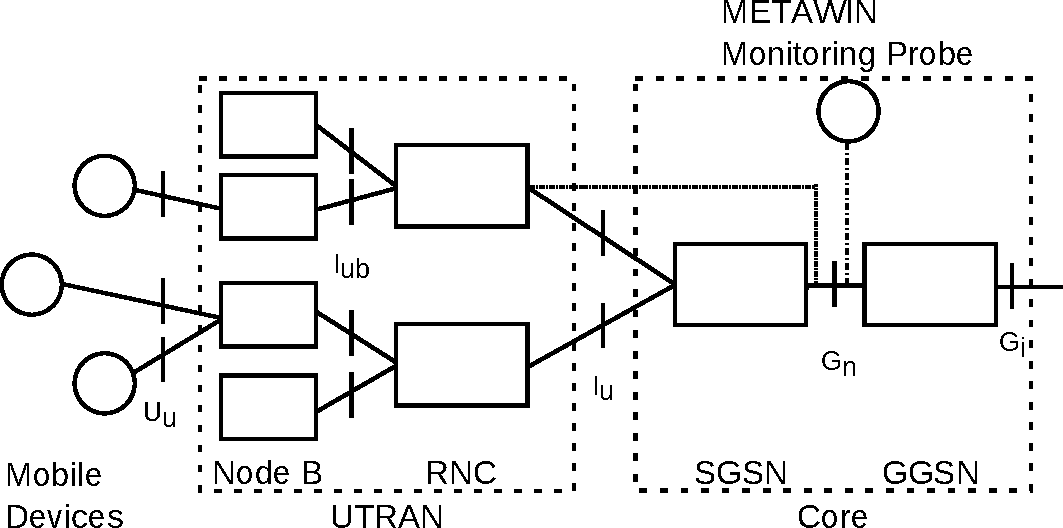
\includegraphics[width=0.7\textwidth]{images/umts-network.pdf}
	\caption{Location of the \acrshort{METAWIN} monitoring probe in the \acrshort{3G} core network.}
\label{c4:fig:umtsnetwork}
\end{figure}

The measurement taps are located at the Gn interface at one \gls{GGSN} within the core network as depicted in Figure~\ref{c4:fig:umtsnetwork}. It gives access to a wide spectrum of core \gls{gtp} signaling, including the mobility and tunnel management. The system does not offer a complete packet trace, but aggregates every signaling transaction and user traffic flow down to a number of select fields. This includes \gls{gtp} \gls{IE} such as the \gls{RAT} as well as the terminal types of the mobile clients. The latter is determinable by the \gls{TAC} part of the \gls{IMEI} and will be discussed later in detail.

In the network under study, a direct link between \glspl{GGSN} and the \glspl{RNC} and circumventing the \gls{SGSN} is present. It is only used for transporting user-plane traffic under specific circumstances, and signaling procedures are still carried out in the normal way between \glspl{SGSN} and \gls{GGSN}. Therefore, only the Gn interface at \gls{GGSN} is seeing the complete core network traffic, which explains the location of the tap. The network under study has more than one \gls{GGSN} at different physical locations. The tapped \gls{GGSN} manages about half of the operator's total traffic volume in this period. 

Recording data in a live network necessitates meeting strict privacy requirements regarding the handling of user-related data. \gls{METAWIN} complies with this by anonymizing all user-identifying. Application-level payload is removed and all user identifiers (e.g. \gls{IMSI}) are non-reversibly hashed before recording. \glspl{UE} in a dataset can still be differentiated by the hashes but not traced back to the actual user. The wiretaps deployed within the monitoring system are time-synchronized with \gls{GPS}. Accordingly, the packet timestamps have an accuracy of least \SI{100}{\nano\second}.


%%%%%%%%%%%%%%%%%%%%%%%%%%%%%%%%%%%%%%%%%%%%%%%%%%%%%%%%%%%%%%%%%%%%%%%%%%%%%%%%
\subsection{Dataset Description}

Using \gls{METAWIN} a week-long core trace was acquired. It was recorded in April 2011, specifically beginning at Monday, \yyyymmdddate\formatdate{10}{4}{2011}, \formattime{0}{0}{0} and ending Sunday, \formatdate{17}{4}{2011}, \formattime{23}{59}{59}.

The trace includes user plane as well as control plane traffic. User plane traffic is recorded in a traffic flow granularity with the trace containing data on \num{2.2e9} aggregated flows. No exact flow start time is given, instead it is rounded down to a \SI{2}{\hour} window with the timestamp at the beginning. A flow entry further consists of hashed identifiers for the gls{IMSI} and the remote server. Besides the usual protocol and port information, the transmitted data volume, in a number of packet as well as byte count, is given on in both link directions. Additional information is available on \gls{HTTP} traffic. This portion of the trace includes precise timestamps as well as the \acrshort{MIME}-type, result code, and size of the requested objected.

The recorded control plane traffic consists of \num{4.1e8} \gls{gtp} tunnel management transactions, i.e., every create, update, and delete request and response. Not all of the \glspl{IE} data is included. But most importantly, it includes the \gls{TAC}, \gls{RAT} and hashed \gls{IMSI} for the purpose of device discrimination. Also present are several timestamps with \SI{64}{\bit} precision describing the time of the request, response and the tunnel's start time. Finally, the \gls{gtp} data contains the response codes for each request. With these codes, failed transactions can be distinguished from successful ones and examined separately. Since the hashed \gls{IMEI} is consistent across the user and control plane data, both can be cross-correlated.

All trace information was exported from \gls{METAWIN} as pure line-based text data. For this investigation all records were fed into a \acrshort{SQL} database. Evaluations were conducted through scripted queries on the database using Python scripts and further statistically evaluated in R.

%%%%%%%%%%%%%%%%%%%%%%%%%%%%%%%%%%%%%%%%%%%%%%%%%%%%%%%%%%%%%%%%%%%%%%%%%%%%%%%
\subsection{Device Identification}

Individual device types in a mobile network can be identified in the data through the \gls{TAC} field on every entry. The \gls{TAC}, defined in \cite{3gpp.23.003}, represents the first eight decimal digits of the \gls{IMEI} and uniquely identifies each device type. The following six digits of the \gls{IMEI} constitute the serial number of a specific device, which is of course omitted in the data. Due to the short length of this serial number, popular devices will often be assigned more than one \gls{TAC}, somewhat complicating the identification of certain device models.

\glspl{TAC} are assigned to individual device models by the regional members, or \gls{RBI}, of the \gls{GSMA}, distinguished by the first two digits of the \gls{TAC}. The full allocation information is not freely available, but only to members of the \gls{GSMA}, which is not a viable option for research institutions and other interested parties. Some independent efforts have been made to collect \glspl{TAC} from devices. Most of them allow just low-volume queries for specific \glspl{TAC} for non-commercial purposes. However, one \gls{TAC} dataset is publicly available and can be used freely.\footnote{Available at: \url{http://www.mulliner.org/tacdb/}.}

This evaluation uses this dataset with some additional device identifiers and classification annotations collected during the course of the investigation. With this at hand, many of the devices associated with the flows and \gls{gtp} messages from the trace were iteratively identified and categorized.


%%%%%%%%%%%%%%%%%%%%%%%%%%%%%%%%%%%%%%%%%%%%%%%%%%%%%%%%%%%%%%%%%%%%%%%%%%%%%%%%
\subsection{\texorpdfstring{\acrshort{TAC}}{TAC} Evaluation Validity}

It is important to know whether the information available in the \gls{TAC} dataset covers enough of the devices seen in the traces to conduct sufficiently meaningful evaluations. After all, the \gls{TAC} data is large but might still be very incomplete due to the sheer number of devices in existence.

\begin{table}
\centering
\caption{Relative \acrshort{TAC} statistics.}
\label{c4:tbl:tacstats}
	\begin{tabu}{XX[r]}
		\toprule
		\textbf{Type} & \textbf{Relative number of devices with an entry in the \gls{TAC} dataset}\\ 
		\midrule
		Total number of flows & \SI{99.72}{\percent} \\
		Ratio of total traffic & \SI{99.97}{\percent} \\
		Total number of tunnels & \SI{87.57}{\percent} \\
		Total number of \gls{gtp} signaling messages & \SI{90.95}{\percent} \\
		Number of distinct \glspl{UE} & \SI{80.93}{\percent} \\ 
		\bottomrule
	\end{tabu}
\end{table}

Table~\ref{c4:tbl:tacstats} provides statistics on the devices that could be identified in the trace. About \SI{81}{\percent} of all unique \gls{TAC} present in the trace could be mapped to a known device. More importantly, when looking at the total number of tunnels and \gls{gtp} messages during the week, even \SI{91}{\percent} of the responsible device can be determined. Finally, the flow data shows an even clearer picture, as almost all of the devices involved can be identified.

This is an interesting result in itself, as the \SI{19}{\percent} of devices present in the dataset that could not be identified through the \gls{TAC} are the cause for only about \SI{9}{\percent} of signaling and \SI{0.3}{\percent} of total traffic. This means there is a long tail of device types in this mobile network with very little impact on the load. With these results, one can be rather confident that evaluations using device discrimination based on this \gls{TAC} mapping should give viable results.


%%%%%%%%%%%%%%%%%%%%%%%%%%%%%%%%%%%%%%%%%%%%%%%%%%%%%%%%%%%%%%%%%%%%%%%%%%%%%%%%
\subsection{Device Classification}

With these device-to-\glspl{TAC} mappings available, additional meta-information can now be added to it, intended to distinguish some of the described load influencing factors. Knowing the model gives also a good knowledge of the device's category and of the \gls{os} it is running by default.\footnote{The \gls{os} actually running on the device at the time of the measurement can not be inferred on this way. But the number of devices running a different \gls{os} than the one installed by default should be relatively low.}

The device's category represents a general classification of the device and should give some initial hints on the fields of use. The devices are partitioned into smartphones, feature phones, \gls{3G} USB dongles or \gls{3G}+WiFi routers, and all other devices. The term feature phone usually points at low-end mobile phones with at least some kind of data capability, often with a physical numerical keyboard. Phones, that could subjectively fall into either the smartphone or the feature phone category were generally attributed as smartphone. Not covered here are any kind of \gls{M2M} devices, because the \gls{TAC} mappings are very inconclusive and incomplete in this area.

The next classification variable is the \gls{os}. Most popular in the trace were the two dominant smartphone \glspl{os}, Android and iOS, and Symbian\footnote{While not completely accurate phones running Series 40 were also attributed to this category because of their close relationship.}, often found on feature phones. Other systems of note are Blackberry OS and Windows Phone or Windows Mobile, but they occur in such a low volume in the trace, that it was decided to completely neglect them and count them towards the other and unknown devices. It should also be noted, that USB dongles and routers cannot be linked to any specific \gls{os} solely by the knowledge of the \gls{TAC}. Also not distinguishable are the exact release versions of the \gls{os} on a specific device. This could diminish the evaluations, as the network behavior could change noticeably between two major versions.

With this knowledge, one can even conjecture on the applications running on the device. Combining the \gls{os} with lists of the most popular applications for this platform can already give some very helpful hints on what can be expected from the traffic mix these types of devices are generating. One final possible \gls{TAC} classification could be a categorization by the phone vendor. However, this was not conducted because it can be safely assumed that the impact is negligible in comparison to the device type and \gls{os}.


%%%%%%%%%%%%%%%%%%%%%%%%%%%%%%%%%%%%%%%%%%%%%%%%%%%%%%%%%%%%%%%%%%%%%%%%%%%%%%%%
\subsection{Preliminary Device Statistics}

After applying the categorization to the network dataset device composition was evaluated to get a first grasp of the network's makeup and to help understand the later investigations.

As expected, the two largest observed portions of devices are smartphones and \gls{3G} dongles, while classic feature phones do not seem to play a major role anymore. About twice as many Android as iOS devices are present, possibly attributed either to the contractual situation of the operator or the wider price range of Android devices.

Regarding traffic, feature phones have negligible user traffic despite still making up one tenth of the device fraction. The difference between \gls{3G} dongles and smartphones is also noteworthy. While the former cause large amounts of user plane traffic (compared to the device numbers), they are responsible for but a few core network signaling events and tunnels. This picture is reversed for smartphones.

One observation across all device types is that about \SI{14}{\percent} of all mobile devices have activated their \gls{GPRS} data service and \gls{gtp} tunnel and cause signaling traffic, but do not initiate any user plane traffic at all.


%%%%%%%%%%%%%%%%%%%%%%%%%%%%%%%%%%%%%%%%%%%%%%%%%%%%%%%%%%%%%%%%%%%%%%%%%%%%%%%
%!TEX root = ../../dissertation.tex
%%%%%%%%%%%%%%%%%%%%%%%%%%%%%%%%%%%%%%%%%%%%%%%%%%%%%%%%%%%%%%%%%%%%%%%%%%%%%%%%
\section{Mobile Core Signaling Evaluation}
\label{c4:sec:evaluations}

Finally, the core network control plane load evaluations can now be tackled. The previously described dataset is thoroughly investigated several approaches to measure load and related factors are iterated.


%%%%%%%%%%%%%%%%%%%%%%%%%%%%%%%%%%%%%%%%%%%%%%%%%%%%%%%%%%%%%%%%%%%%%%%%%%%%%%%%
\subsection{Traffic Ratio Estimations}

\begin{table}
\centering
\caption{Relative device-discriminated traffic statistics extracted from the dataset.}
\label{tab:trafficstats}
	\begin{tabu}{X[1.4]X[r]X[r]X[r]X[r]X[r]}
	\toprule
	& \textbf{Flows} & \textbf{Traffic} & \textbf{Tunnels} & \textbf{\gls{gtp} messages} & \textbf{Devices}\\ 
	\midrule
	\multicolumn{2}{c}{\textbf{By device type}}       &             &             &             &           \\
	% In TAC DB      & $99.72\%$   & $99.97\%$   & $87.57\%$   & $90.95\%$   & $80.93\%$ \\
	Smartphones      & $20.58\%$   & $12.81\%$   & $60.31\%$   & $75.99\%$   & $37.97\%$ \\
	Regular phones   & $0.26\%$    & $0.37\%$    & $5.40\%$    & $0.94\%$    & $9.25\%$  \\
	\gls{3G} dongles & $66.55\%$   & $75.12\%$   & $12.71\%$   & $9.53\%$    & $25.10\%$ \\
	\midrule
	\multicolumn{2}{c}{\textbf{By \gls{os}}}       &             &             &             &           \\
	Android          & $10.82\%$   & $6.48\%$    & $14.33\%$   & $43.33\%$   & $14.01\%$ \\
	iOS              & $7.22\%$    & $4.47\%$    & $18.91\%$   & $20.35\%$   & $7.94\%$  \\
	Symbian          & $1.02\%$    & $1.09\%$    & $21.17\%$   & $4.51\%$    & $12.97\%$ \\
	Blackberry OS    & $0.07\%$    & $0.10\%$    & $2.17\%$    & $2.60\%$    & $1.48\%$  \\
	\bottomrule
	\end{tabu}
\end{table}

To get a first grasp of the dynamics present in the dataset and the core network under investigation, Table~\ref{tab:trafficstats} shows a small survey of the traffic composition split up by device type and \gls{os} categories. The majority of signaling messages originated from smartphones, which in turn generated only a small portion of user traffic when compared to \gls{3G} dongles.

With these numbers, the notion of active devices or tunnels can also be introduced. This only includes entities that, besides signaling, actively generated user traffic during their life cycle. Interestingly, only about \SI{82}{\percent} of all unique devices in the trace were active and could be associated with at least one traffic flow. The remaining \SI{18}{\percent} of devices still had an open \gls{gtp} tunnel but never used it. This is an extreme for the core network, as it causes a significant amount of control plane load without any actual benefit to either the network or the device. The active device distinction will also be used later on in the evaluation.

Unfortunately, the dataset does not contain any hard numbers on the volume of the signaling messages, which could be a direct indicator of the network load the control plane imposes. But using the estimation of the upper limit of a \gls{gtp} message from Section~\ref{c4:sec:gtp}, a rough upper limit on the total signaling traffic can also be derived. The following formula is used:

\begin{align}
	\phantom{,}v_s &= 2\left|S\right|(v_{gtp} + v_{udp} + v_{ip})\text{,}\\
	\phantom{.}t_r &= \frac{v_s}{v_t} \approx 0.7\si{\percent}\text{,}
\end{align}
%
with the signaling volume $v_s$, the set of signaling messages $S$, the estimated size of a \gls{gtp} message $v_s$, and the length of the \gls{UDP} and \gls{IP} headers. In this scenario, the traffic ratio $t_r$ of $v_s$ compared to the total traffic $v_t$ is calculated to be a minute \SI{0.7}{\percent}. Therefore, it can be safely assumed that the volume of control plane traffic appears to be a non-issue and not the bottleneck. The other load factors at the network nodes described earlier must play a more critical role, such as the memory profile of the states kept in the gateway nodes, the time required to process the large number of information held in the messages, or the imposed latency through several message round trips during transactions.

This is why the following evaluations are all intended to find some indirect approach to measure the system's load.



%%%%%%%%%%%%%%%%%%%%%%%%%%%%%%%%%%%%%%%%%%%%%%%%%%%%%%%%%%%%%%%%%%%%%%%%%%%%%%%%
\subsubsection{\texorpdfstring{\acrshort{gtp}}{GTP} Tunnel Duration}

The first indirect evaluation target will be the duration of the \gls{gtp} tunnels. This duration is directly related to the amount of occurring tunnel management signaling between the \gls{SGSN} and \gls{GGSN}. In turn, each of these signaling interactions causes processing at the two involved nodes and changes the amount of state in the form of the \gls{PDP} context. In terms of signaling messages, looking at the duration catches both tunnel create and delete messages, but no update message.

For the purpose of the evaluation the duration is defined as the interval between corresponding \gls{gtp} create and delete messages. As soon as the \gls{GGSN} sends its successful response to the create request, it can be expected that the necessary state has been created throughout the \gls{CN} and is ready to forward user packets. Similarly, after a delete message, user traffic should not be forwarded anymore. However, state may still exist and could be freed up lazily. But the latter depends entirely on the specific implementation.

As a side note, while the trace itself is only one week long, information on tunnels longer than this period can still be obtain when they were closed during the period. The trace's record on delete messages also contains the timestamp of the initial tunnel creation.

All the individual tunnel durations in the dataset are differentiated based on two factors based on the presented \gls{TAC} mechanics. The first part of the investigation looks at tunnels from different device types. After that, possible influences from the operating system are investigated. 


%%
\paragraph{Influence of the Device Type}

\begin{figure}[htb]
	\centering
	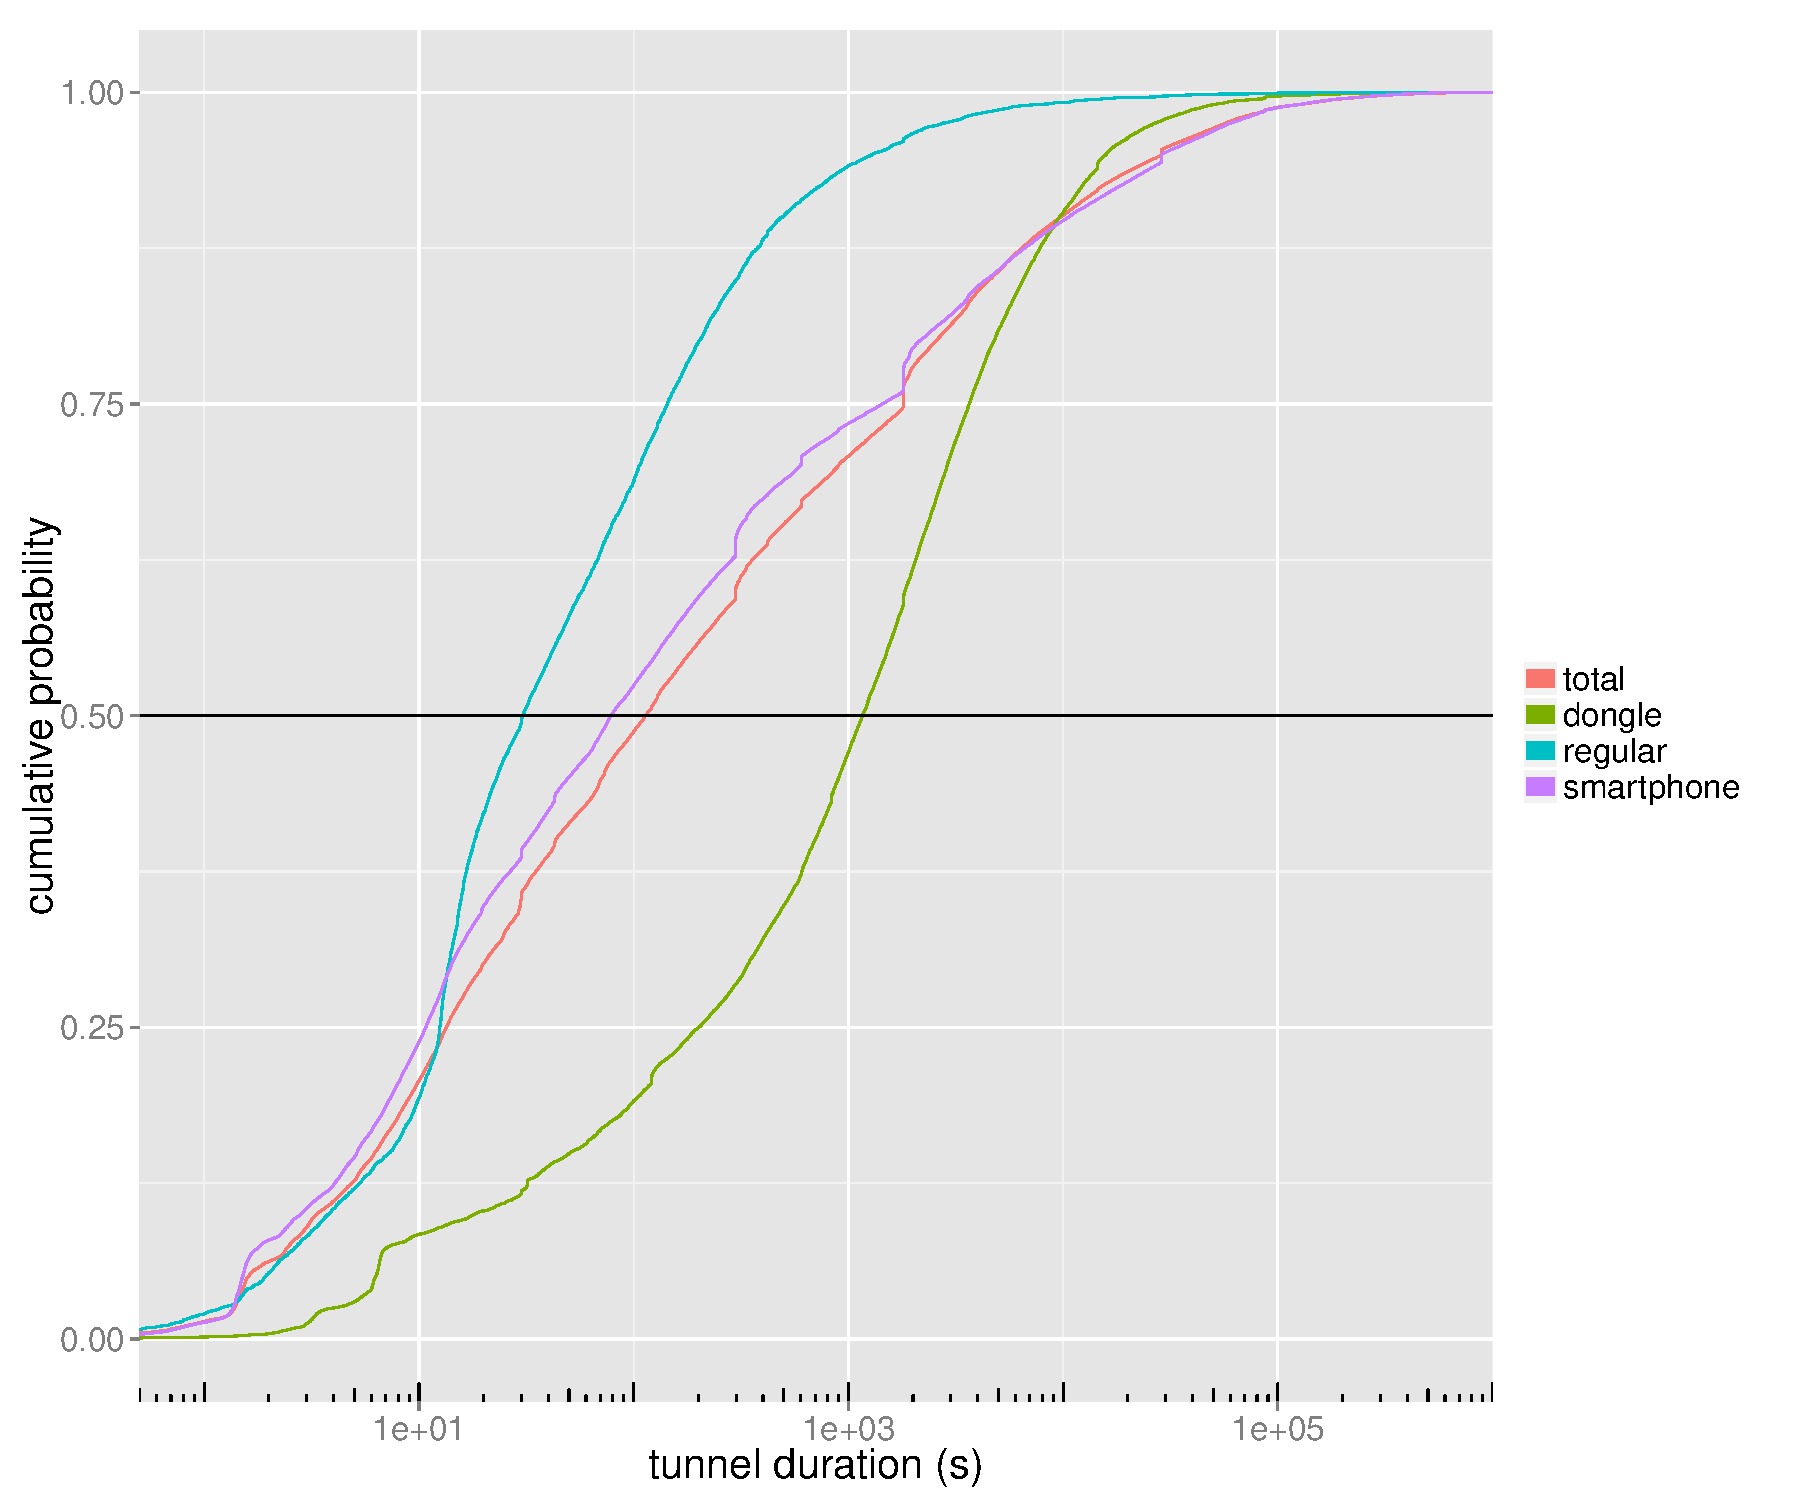
\includegraphics[width=0.9\textwidth]{images/R-tunnel-duration-device-type.pdf}
	\caption{Tunnel duration distribution, separated for \acrshort{3G} dongles, smartphones and regular phones with medians at \SI{115}{\second} (total), \SI{31}{\second} (regular), \SI{82}{\second} (smartphone), and \SI{1207}{\second} (dongle).}
\label{c4:fig:cdf-duration-device-class}
\end{figure}

Figure~\ref{c4:fig:cdf-duration-device-class} shows the \gls{ECDF} for the user tunnels and their \gls{PDP} Context durations in the dataset. In this first graph, the duration of different device classes is distinguished and put in perspective to the overall duration distribution. The devices classes here are smartphones, regular phones, and \gls{3G} dongles. It can be observed that tunnel durations range between seconds and more than one week.

The median can be clearly differentiated between device types, being much longer for \gls{3G} dongles than for mobile phones. This reflects expected user behavior very well and gives a first indicator on a possible influence of the user plane on the control plane.

Dongles are usually used with laptops to be able to work while being mobile. Dongle sessions last therefore often for extended periods longer than a few minutes up to hours. Also, this type of device is usually put into a standby mode after the period, which completely disables any mobile connections --- and therefore any associated tunnel --- instead of switching to low power radio idle modes. This is reflected in the dongle tunnel duration here as well. When compared to the other device category, dongles are more compactly centered around their median of about \SI{20}{\minute}.

A similar behavior can be observed in the regular phone distribution with values arranged tightly around the median of \SI{31}{\second}. Compared to today's smartphones, data connections on regular phones are mostly initiated explicitly by user interaction, for example through starting a browser and viewing a web page. This could also explain the comparatively low durations here.

The picture is rather different in the smartphone tunnel duration. Here, often background tasks are running over long periods of time and devices try to keep connectivity up as long as possible (while still attempting to conserve power). Overall, this could lead to the smoother distribution seen here with no clear center value.

Overall, a relatively high number of tunnels with a duration shorter than \SI{10}{\second} can also be observed. Especially the peak at about \SI{1.5}{\second} --- which is interestingly shifted to \SI{6.8}{\second} in the dongle distribution --- is of note. This is even shorter than the default values for the \gls{RRC} idle state transitions which causes the tunnel to be destroyed. It can be conjectured that these short tunnels have been explicitly removed by the \gls{UE} as no other involved state machine has timers this short.

Another distinct step at \SI{30}{\minute} in the total and smartphone distributions can be observed. As it is only present in these to categories --- and the total distribution looks to be mostly governed by smartphones --- it is reasonable to assume that the cause for this is a specific behavior observable in some aspect of smartphone related influence factors.


%%
\paragraph{Influence of the \texorpdfstring{\acrshort{os}}{OS}}

\begin{figure}[htb]
	\centering
	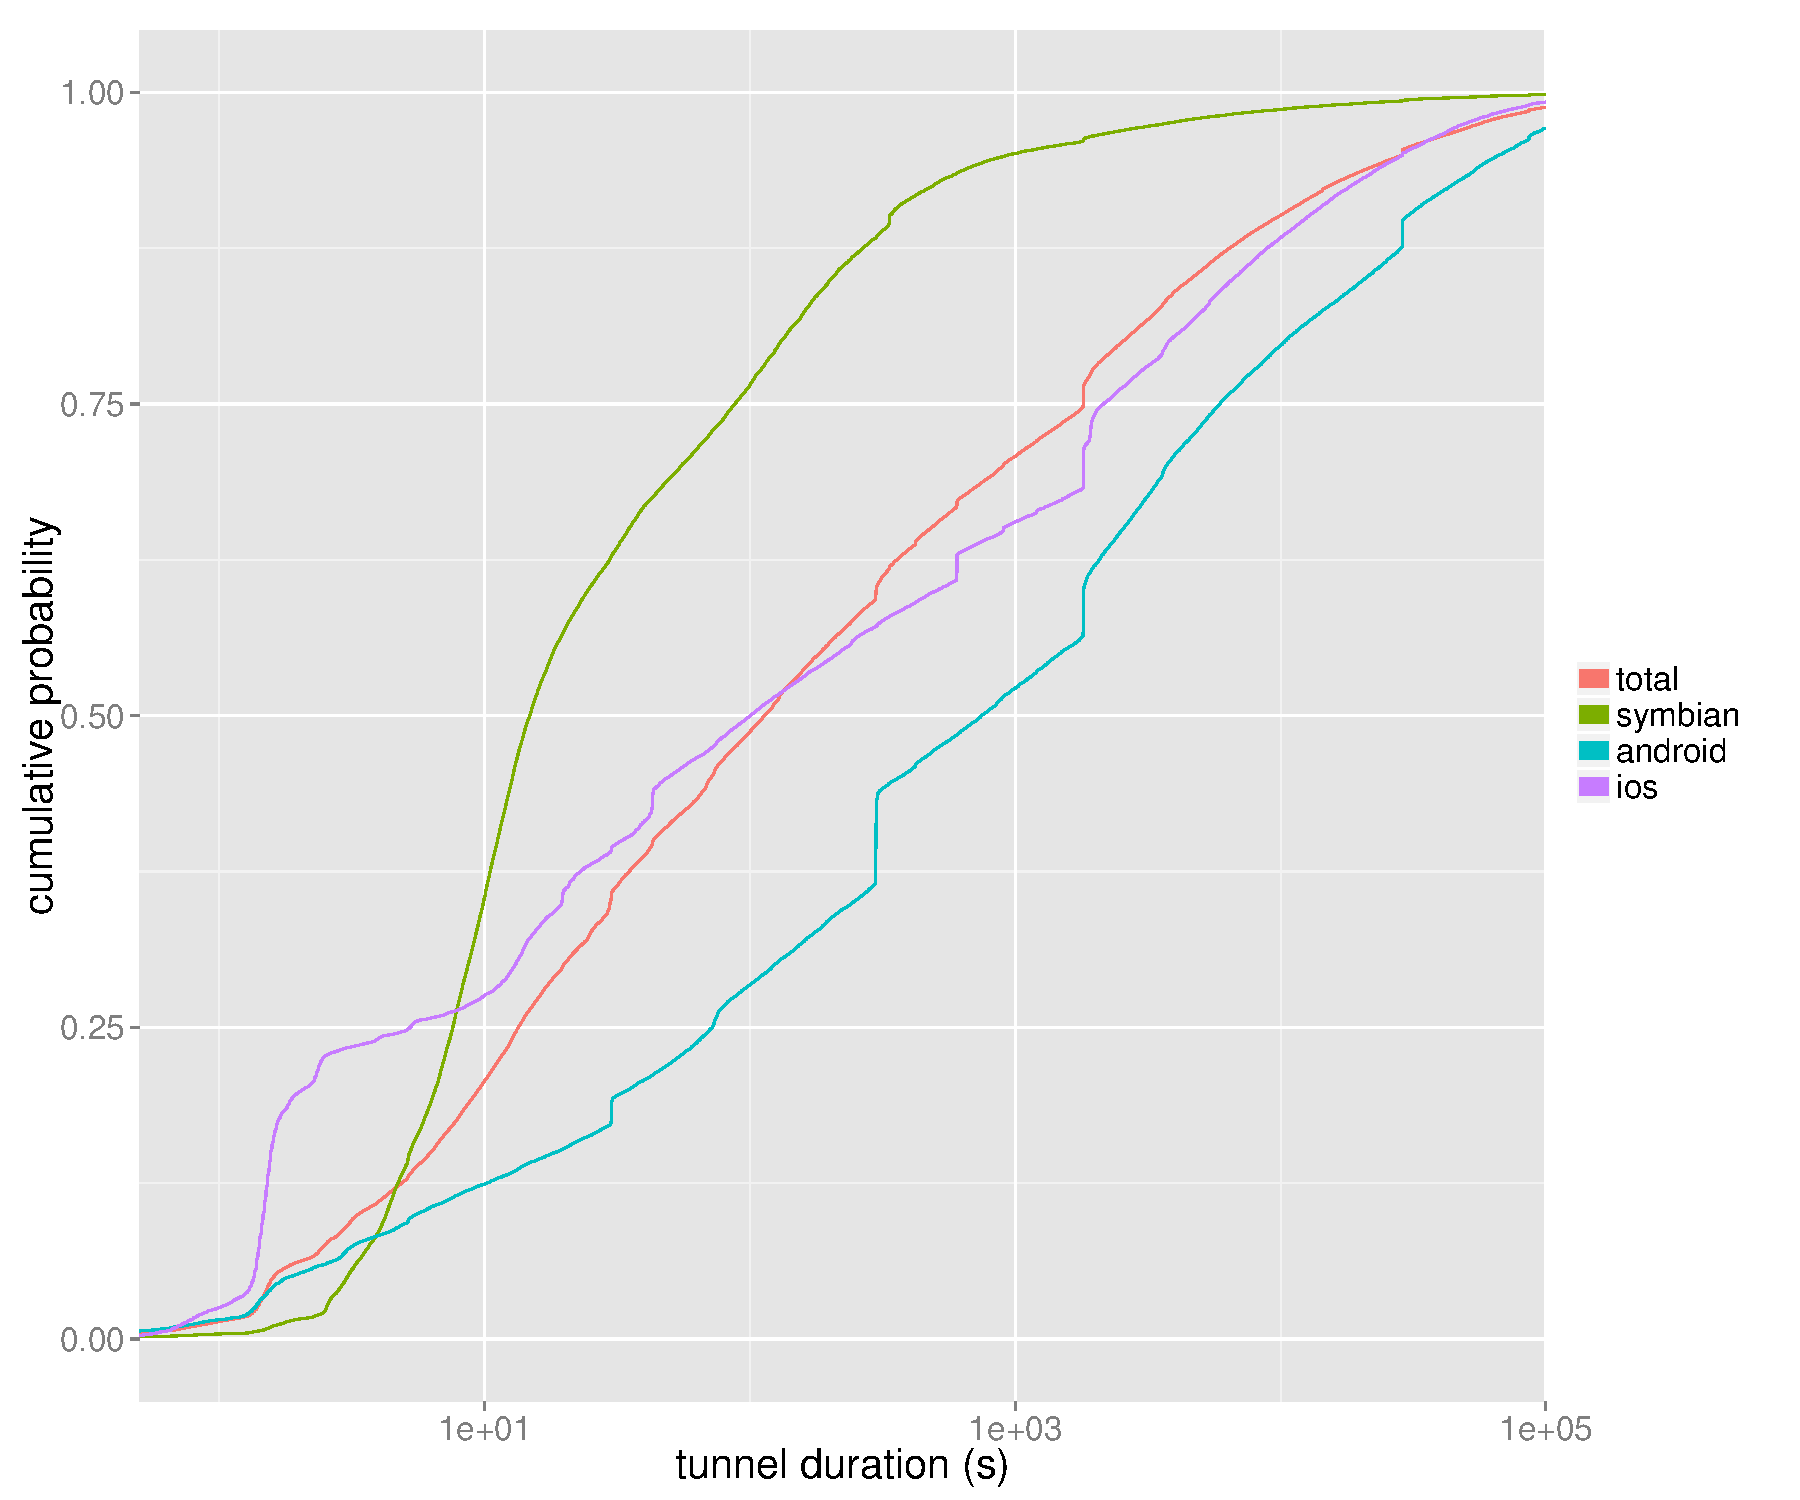
\includegraphics[width=0.9\textwidth]{images/R-tunnel-duration-operating-system.pdf}
	\caption{Tunnel duration \acrshort{CDF}, separated for select \acrshortpl{os}; Medians at \SI{115}{\second} (total), \SI{15.5}{\second} (symbian), \SI{104}{\second} (iOS), and \SI{765}{\second} (android).}
\label{c4:fig:cdf-duration-os}
\end{figure}

Next, the two phone categories are further broken down by their \gls{os}. Only the three major systems, Android, iOS, and Symbian, are identified here, the amount of other types was negligible. The smartphone category is almost exclusively represented by Android and iOS devices, while Symbian devices make up most of the regular phones but is also represented in a number of smartphone models.

Figure~\ref{c4:fig:cdf-duration-os} depicts the \gls{ECDF} of the tunnel durations of these categories in relation to the total duration distribution. They immediately exhibit a clear difference between individual \glspl{os}.

The Symbian tunnel durations are similarly distributed to the previously depicted regular phone category, albeit with an even shorter duration median of about \SI{15}{\second}. This is an indicator of the large intersection between these two groups and the explicit user traffic property attributed to regular phones.

The two smartphone-exclusive \gls{os} have remarkably similar tunnel distributions with the exception of the Android tunnel distribution shifted to much longer tunnels. This is mostly due to the larger accumulation of iOS tunnels around the previously mentioned \SI{1.5}{\second} mark. Over \SI{20}{\percent} of all tunnels established by iOS devices are shorter than \SI{2}{\second}. A possible explanation is an interaction between the described implicit background traffic happening in intervals and the efforts of iOS phones to preserve as much energy as possible. 

To this end, phones aggressively force their radio connection to the low power idle states or even completely shut off the radio immediately after transmission have ended, circumventing \gls{RRC} timers. To achieve this, iOS devices are known to implement a form of \gls{3GPP} Fast Dormancy~\cite{gsma2011fdbestpract}. It is deemed to improve device battery life, radio signaling and radio spectrum efficiency. Due the more frequent state transitions it also could cause an increase in core network tunnel management signaling, which is probably what happened in the iOS case depicted in the \gls{ECDF}.

Another set of tunnel duration accumulations are also visible in the \gls{os} distributions. Two types of steps should be distinguished here. First are accumulations that occur across multiple or all categories. This points to an influence source outside of the specific category. If the artifact is present in every distribution it is even likely that the source is a behavior of the network's state machines. The second type of accumulation is local to one or some categories, which places the root cause into the region of these categories and their related influence factors. 

In case of the \gls{os} category, additionally, peaks at \SI{30}{\second}, \SI{300}{\second}, and \SI{600}{\second} can be observed. However, whether this behavior can be attributed directly to the operating systems themselves cannot be decided just by looking at these distribution. Other factors, e.g., the device's baseband and user traffic dynamics, also play a role. 


%%
\paragraph{Influence of the Time of Day}

\begin{figure}[htb]
	\centering
	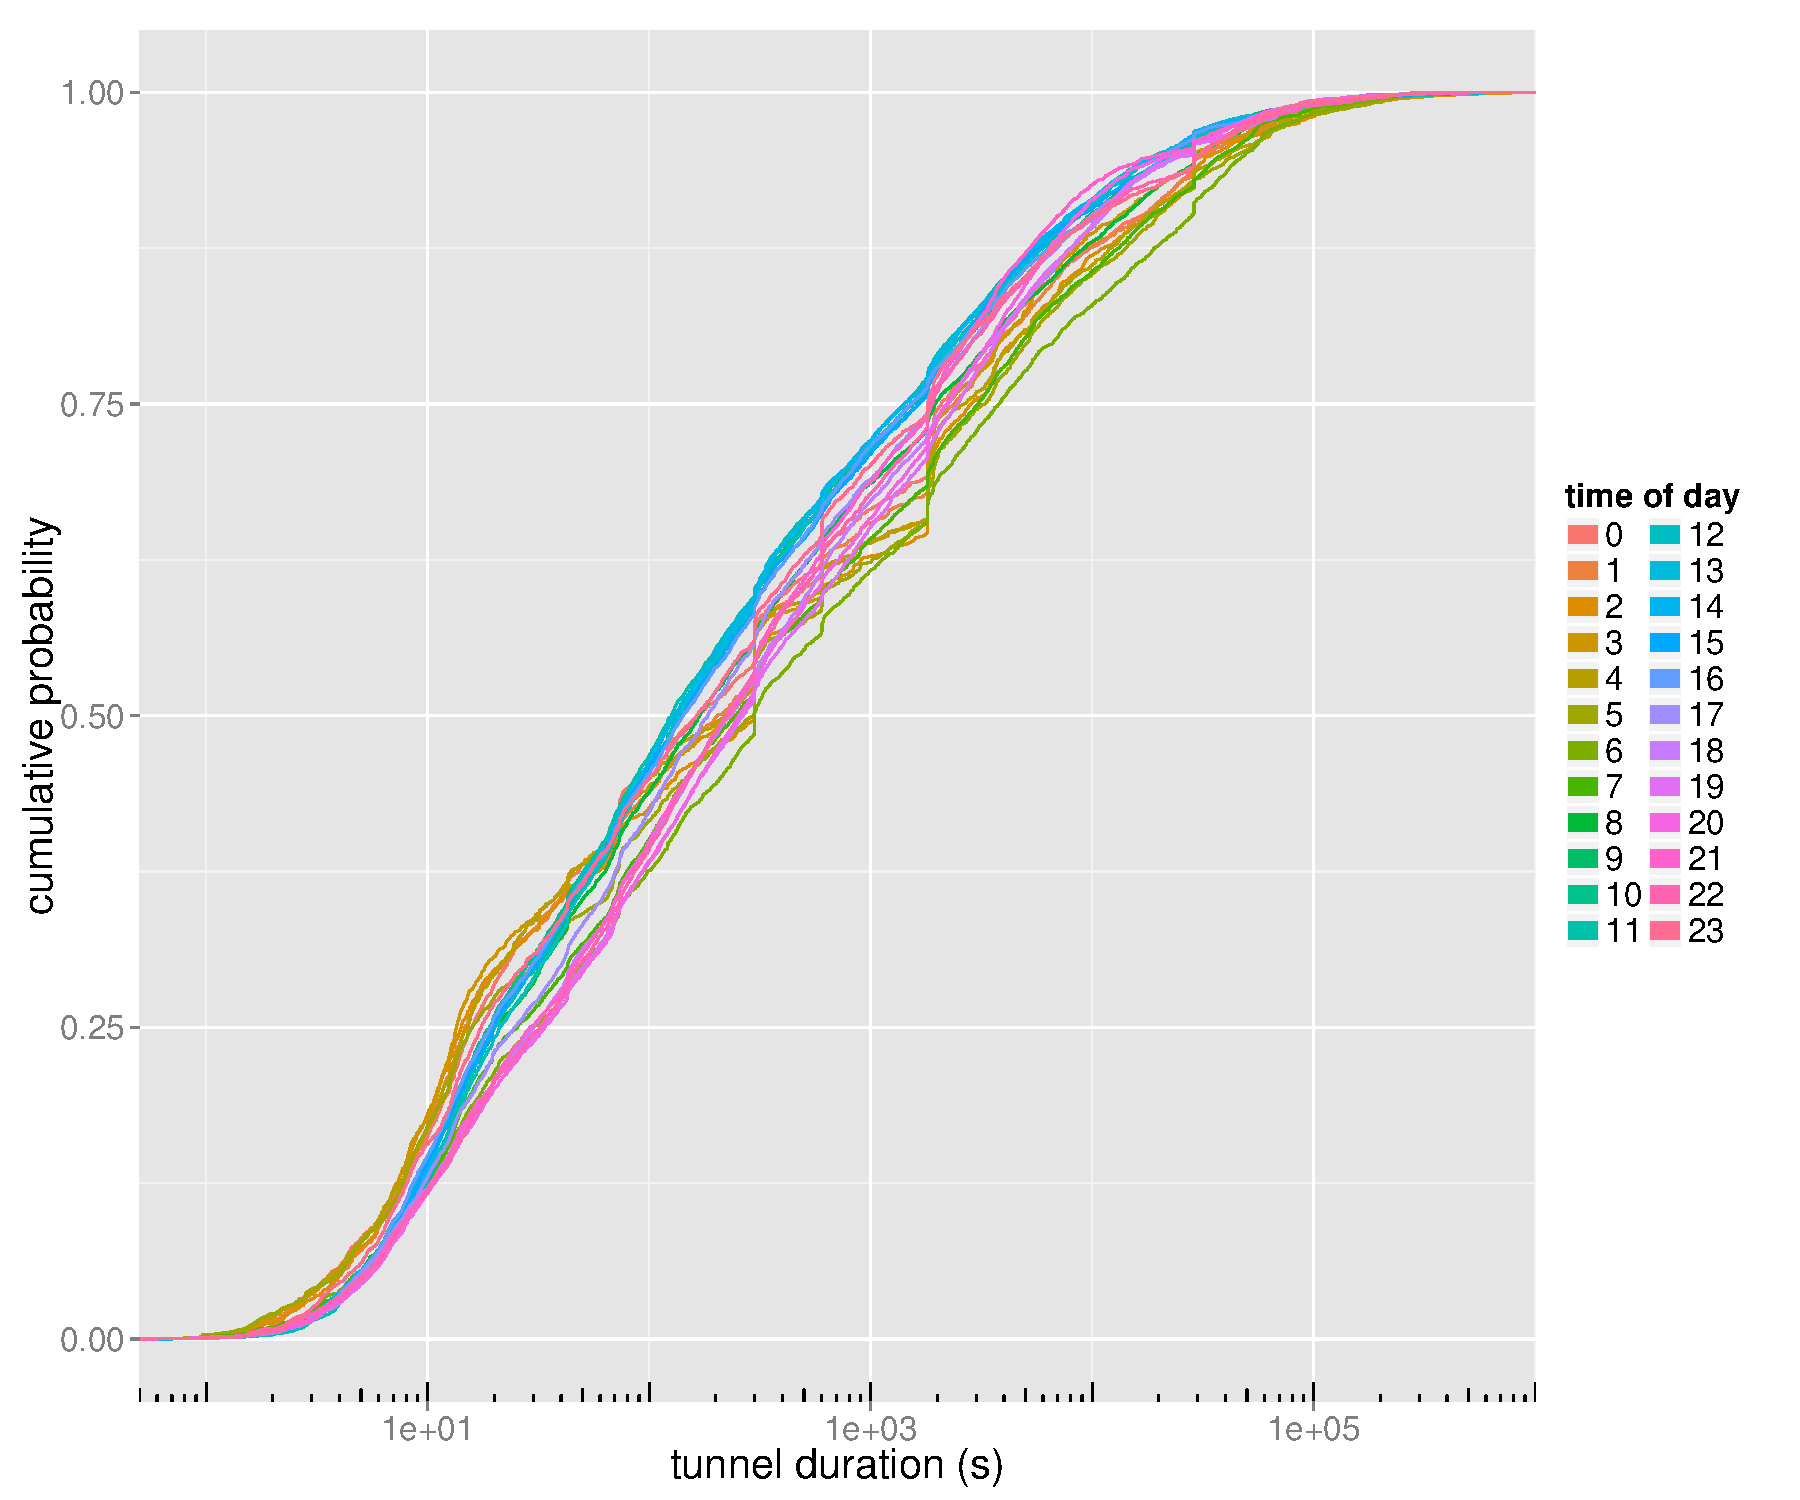
\includegraphics[width=0.9\textwidth]{images/R-duration-timeofday-ecdf.pdf}
	\caption{Tunnel duration of all active tunnels by time of day.}
\label{c4:fig:duration-timeofday-ecdf}
\end{figure}

In addition to device factors, diurnal effects could also play a role in the duration of tunnels. Figure~\ref{c4:fig:duration-timeofday-ecdf} depicts $24$ individual \glspl{ECDF} of the tunnel duration for each hour of a day. While no clear distinctions are visible, there is a trendto shorter tunnels in the early morning hours. The early afternoon hours tend to produce tunnels more centered around the middle duration range. Even longer tunnels should be treated with reservation, as they exceed the length of their assigned time slot in the \gls{ECDF} and span a larger time frame. Only the tunnel creation point is guaranteed to be in the slot.


%%
\paragraph{Influence of Other Factors}

Due to the nature of the trace dataset at hand many other influence factors are hard or outright impossible to distinguish. Some factors are unknown from the \gls{CN} perspective, as the mentioned device baseband, while others have not been recorded in the trace.

For example, it would theoretically be possible to investigate the influence of the \gls{RAT} as it is an \gls{IE} in the \gls{gtp} messages and also recorded in the trace. The radio access parts of \gls{GSM} and \gls{UMTS} are completely different --- including the \gls{RRC} state machines which were depicted in Figure~\ref{c4:fig:mmstatemodel} --- and therefore could also differ in their control plane load impact on the core. However, the \gls{RAT} \gls{IE} is optional and only set in less than \SI{1}{\percent} of the available records. As the radio access can change even during an existing tunnel --- in which case the \gls{GGSN} receives a \gls{gtp} update request informing the node about the change --- a complete picture without gaps would be required to do any investigation on this.


%%
\paragraph{Influence Strength of the Categories}

\begin{figure}[htb]
	\centering
	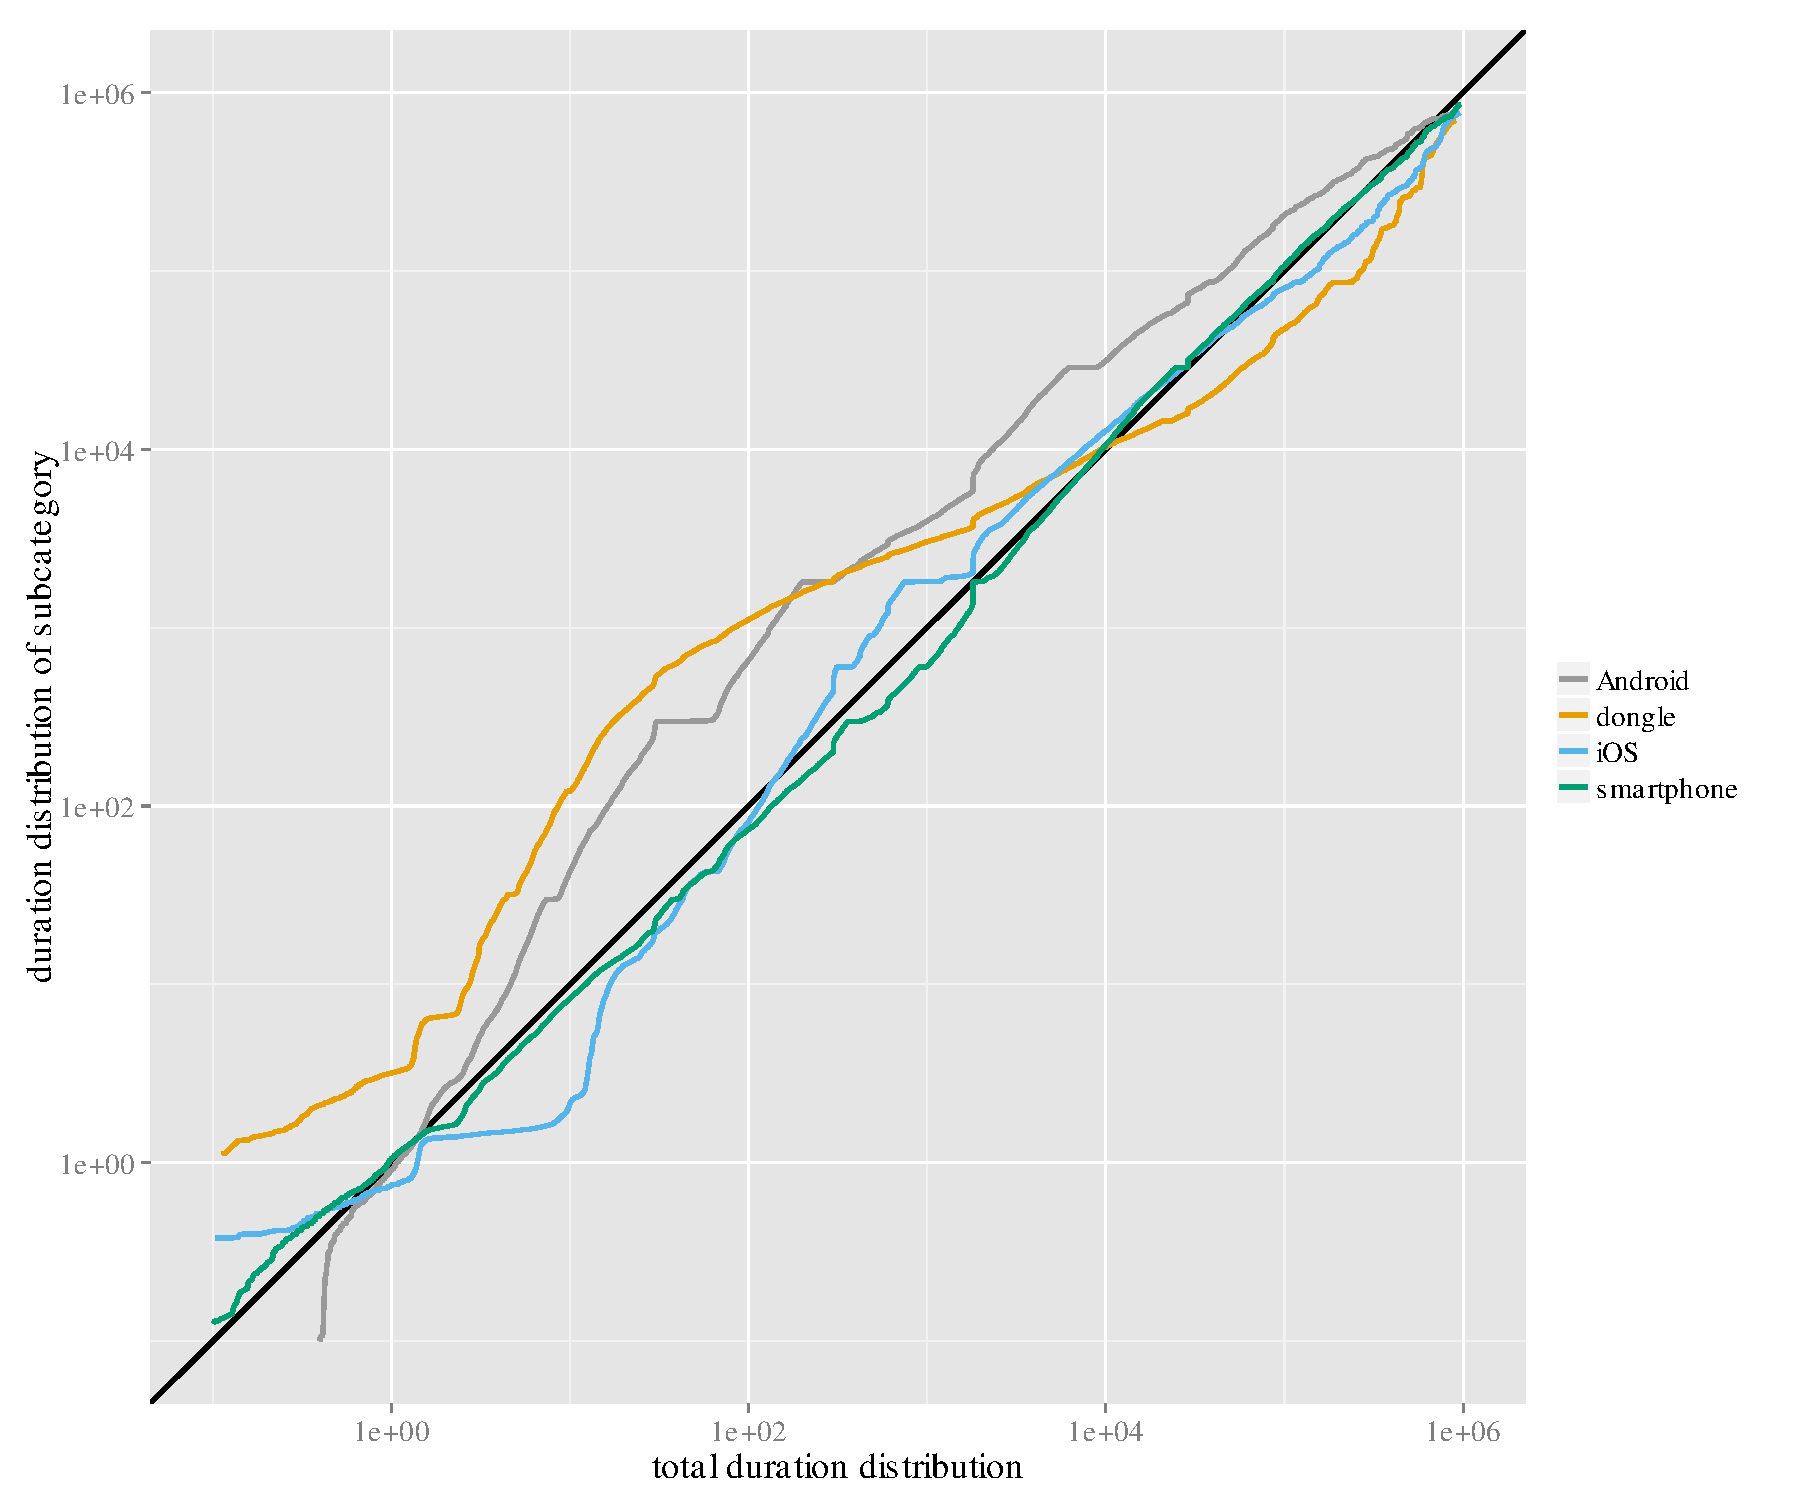
\includegraphics[width=0.9\textwidth]{images/R-duration-qq-category-comparison.pdf}
	\caption{Q-Q Plots of the tunnel duration distributions in comparison to device classification categories.}
\label{c4:fig:qq-plots}
\end{figure}


To ascertain which of the investigated device categories influences the total duration distribution most, Q-Q plots are created and investigated. It is conjectured that the amount of influence on the duration distribution is correlated to the influence on the control plane load. In theory, if both durations follow the same distribution, one expects a straight diagonal $y=x$ line through the origin. A steeper incline indicates more compact regions in the distribution plotted on the $x$ axis and vice versa.

The Q-Q plots in Figure~\ref{c4:fig:qq-plots} compare the total tunnel duration distribution to the duration distribution of the dongle, smartphone, Android, and iOS classification cateogries. It can be observed that the smartphone duration distribution is distributed almost equally to the total except for minor variations. However, the \gls{3G} dongle tunnel durations follow a very different distribution. Their effect on the total duration distribution seems to be negligible despite the  large amount of traffic they are causing. This is also a first indicator that smartphones might have a larger impact on signaling than other device types.

Looking closer at the smartphone category, Q-Q plots of the two major \glspl{os} are investigated. With the exception of the large below \SI{2}{\second} peak in the lower tail of the distribution, iOS device tunnel durations are very similar to the overall tunnel duration distribution. The same can not be said about the Android distribution, which deviates somewhat in the distribution's center but is similar to the total distribution in the upper tail. Even devices with just a different \glspl{os} seem to strongly differ in their influence on duration distribution and therefore on signaling.

\begin{figure}[htb]
	\centering
	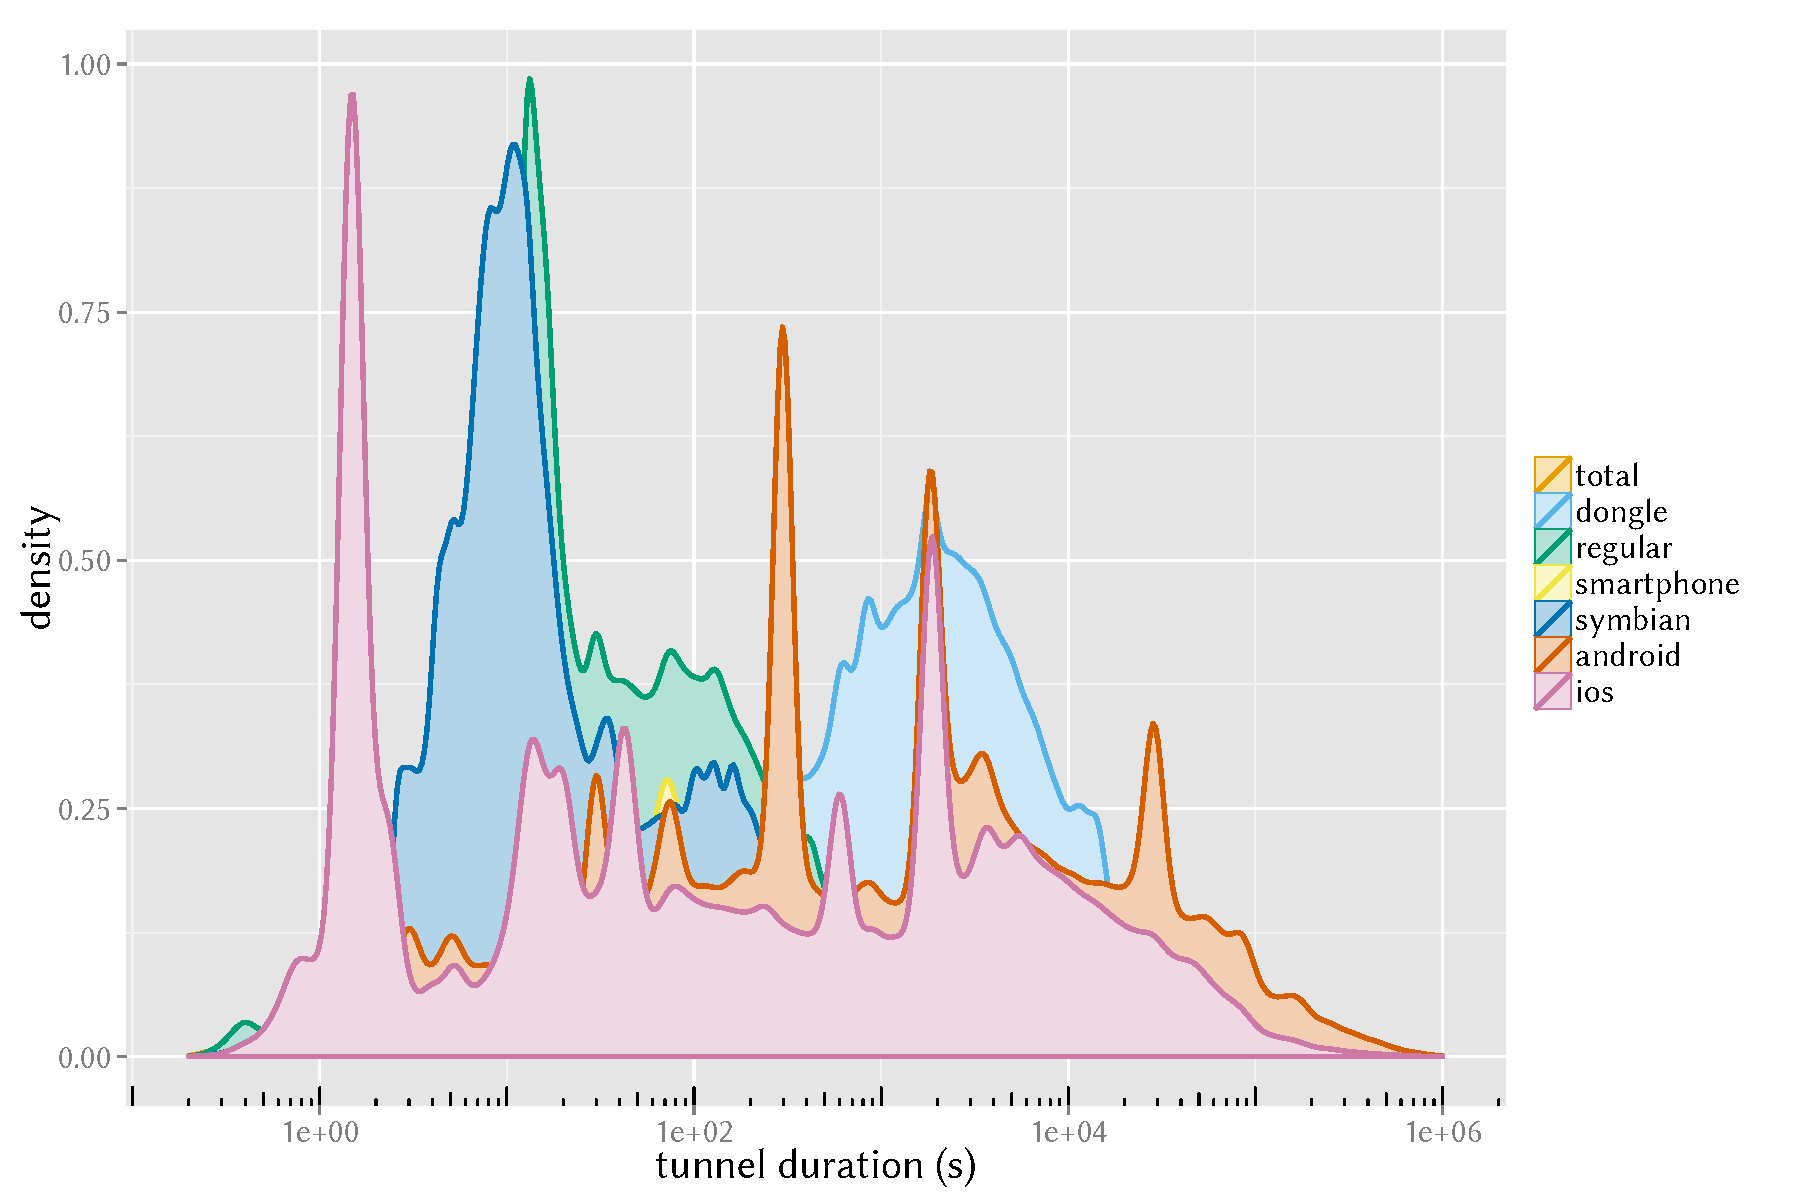
\includegraphics[width=0.9\textwidth]{images/R-duration-classification-density.pdf}
	\caption{Logscale density plot of the tunnel duration with all classifications.}
\label{c4:fig:durations-density}
\end{figure}


Figure~\ref{c4:fig:durations-density} attempts to depict where in their distributions the investigated device categories show the most impact on the total distribution. The plot shows the density of all previously investigated device influence categories.

It is evident that the durations are not evenly distributed, but rather follow sharp spikes. One of largest spike across all categories is the one at a duration of \SI{30}{\minute}, with about \SI{1.8}{\percent} of all tunnels in the network falling into that region. Since this spike happens across all device types, it makes a rather strong case for being induced by the network. On the other hand, the bulk of tunnel durations in the short-to-medium range does not seem to be governed by the two major smartphone operation systems but by other devices in the network, which do not show major spikes in other bins.

Besides the long-tailed behavior in the upper tail of the tunnel durations another slight accumulation effect, repeating itself every \SIrange{6}{7}{\day}, is present in the upper tail. This phenomenon is as yet of unknown origin and does not coincide with any known timers of the \gls{3G} mobile network.

The investigation of this data leads to the conclusion that the planning and dimensioning of the control plane needs to watch the behavior of smartphones more carefully than that device types.


%%%%%%%%%%%%%%%%%%%%%%%%%%%%%%%%%%%%%%%%%%%%%%%%%%%%%%%%%%%%%%%%%%%%%%%%%%%%%%%
\subsubsection{\texorpdfstring{\acrshort{gtp}}{GTP} Tunnel Arrivals}

The duration of \gls{gtp} tunnels is but one aspect of influence on control plane load. The arrival process of these tunnels is also interesting in itself. Specifically, this mean the arrival of tunnel requests, i.e.\gls{gtp} create requests, at the \gls{GGSN}. 

An arrival process can be described in two distinct ways. First by the number of arrivals in a given time interval. Second, by the \gls{IAT}, the time between two consecutive tunnel arrivals. Depending on the choice one has to deal with either a discrete or a continuous distribution.

Here, the tunnel arrival process is investigated with both approaches. This also adds to the foundation of the load model constructed in the next chapter. Note, that the notion of classifying arrivals into influence categories based on device specifics is omitted here. An investigation of this process can not be realistically be conducted categorized and still relate to the total system load.

\begin{figure}[htb]
	\centering
	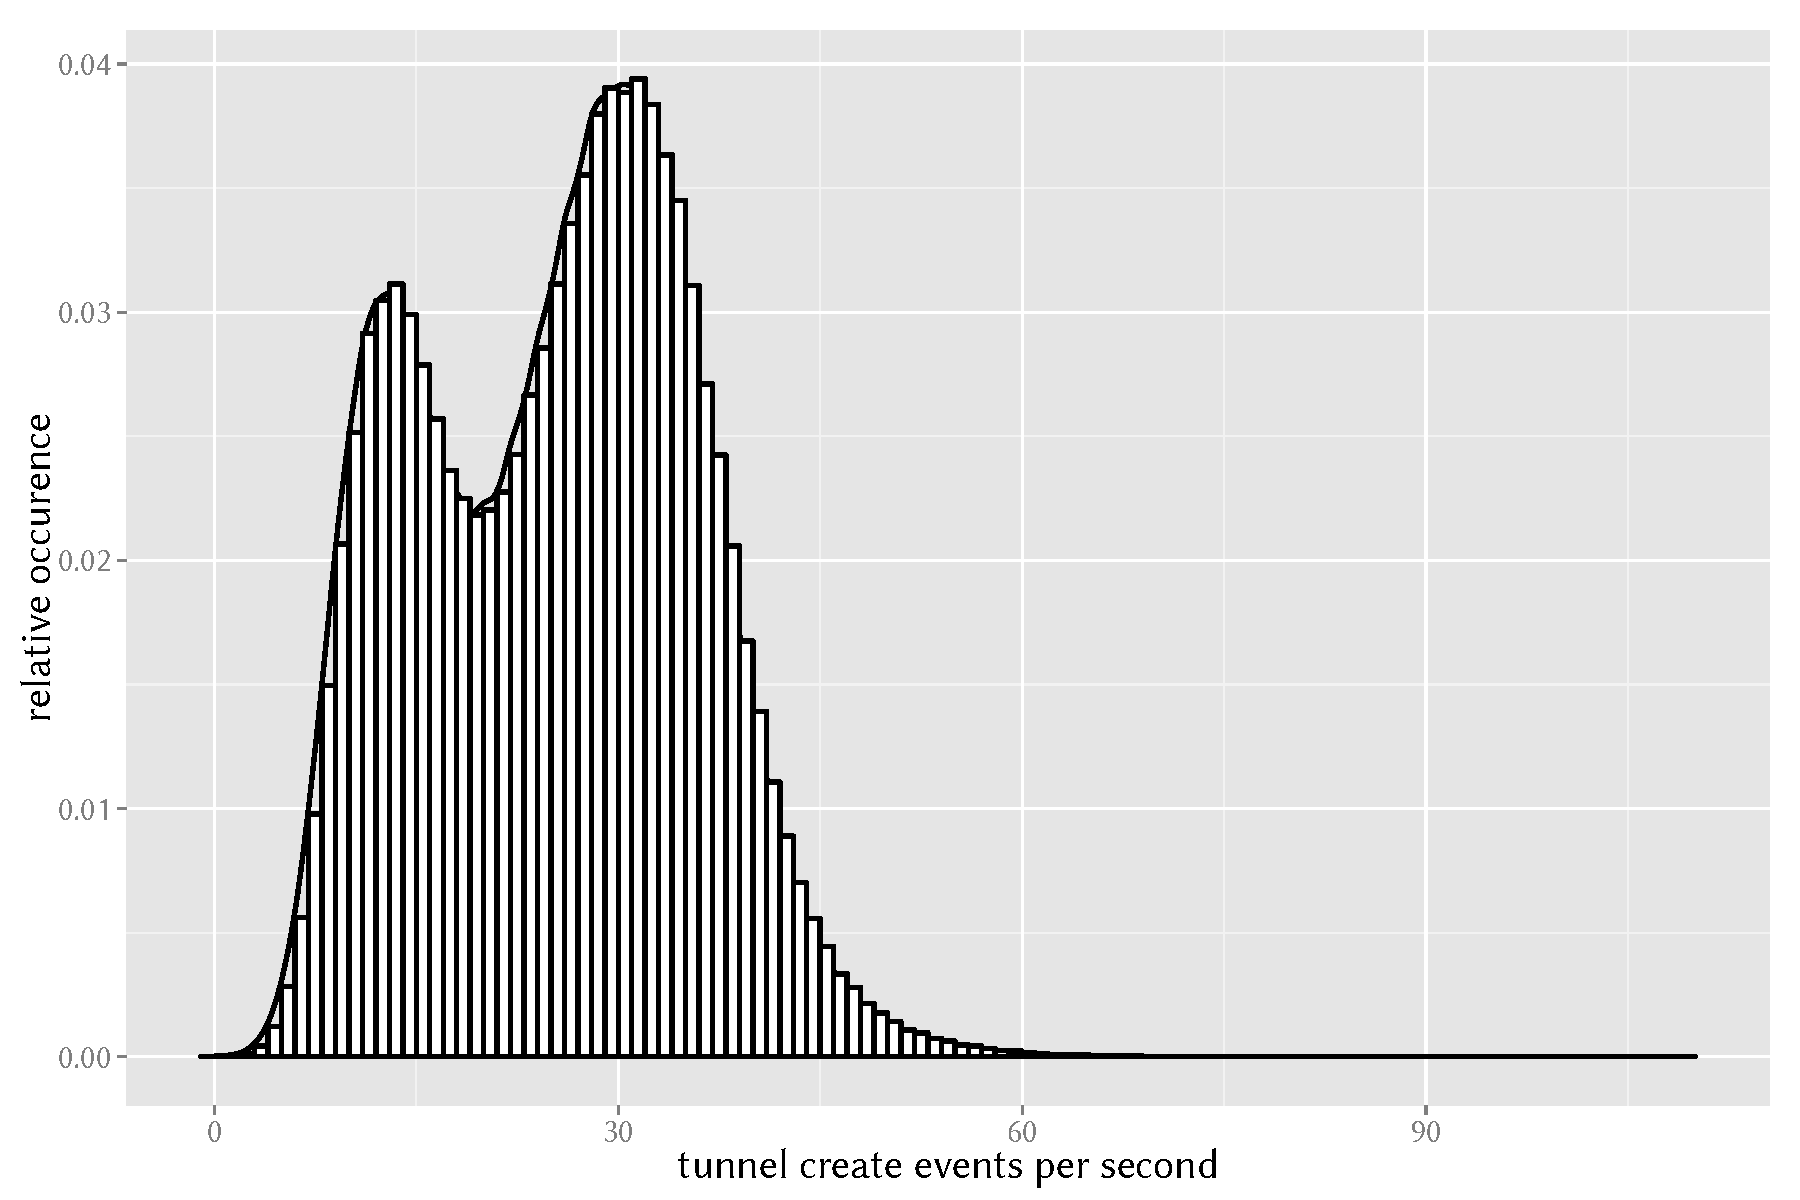
\includegraphics[width=0.9\textwidth]{images/R-create-frequency.pdf}
	\caption{Tunnel arrivals histogram overlaid with a density plot.}
\label{c4:fig:freq-arrivals}
\end{figure}

Figure~\ref{c4:fig:freq-arrivals} depicts a histogram the number of tunnel arrivals per second during the whole trace duration period. Of note is the clear bimodal nature with one peak around twelve and the other in the low thirties. While the distribution is rather compact around these two peaks, there are some clear outliers peaking at $107$ arrivals per second. If the hypothesis of the correlation between signaling load and number of arrivals holds, it can be assumed that load is not constant but rather switches between two modes with some periods of very high load induced by an increased number of arrivals.

\begin{figure}[htb]
	\centering
	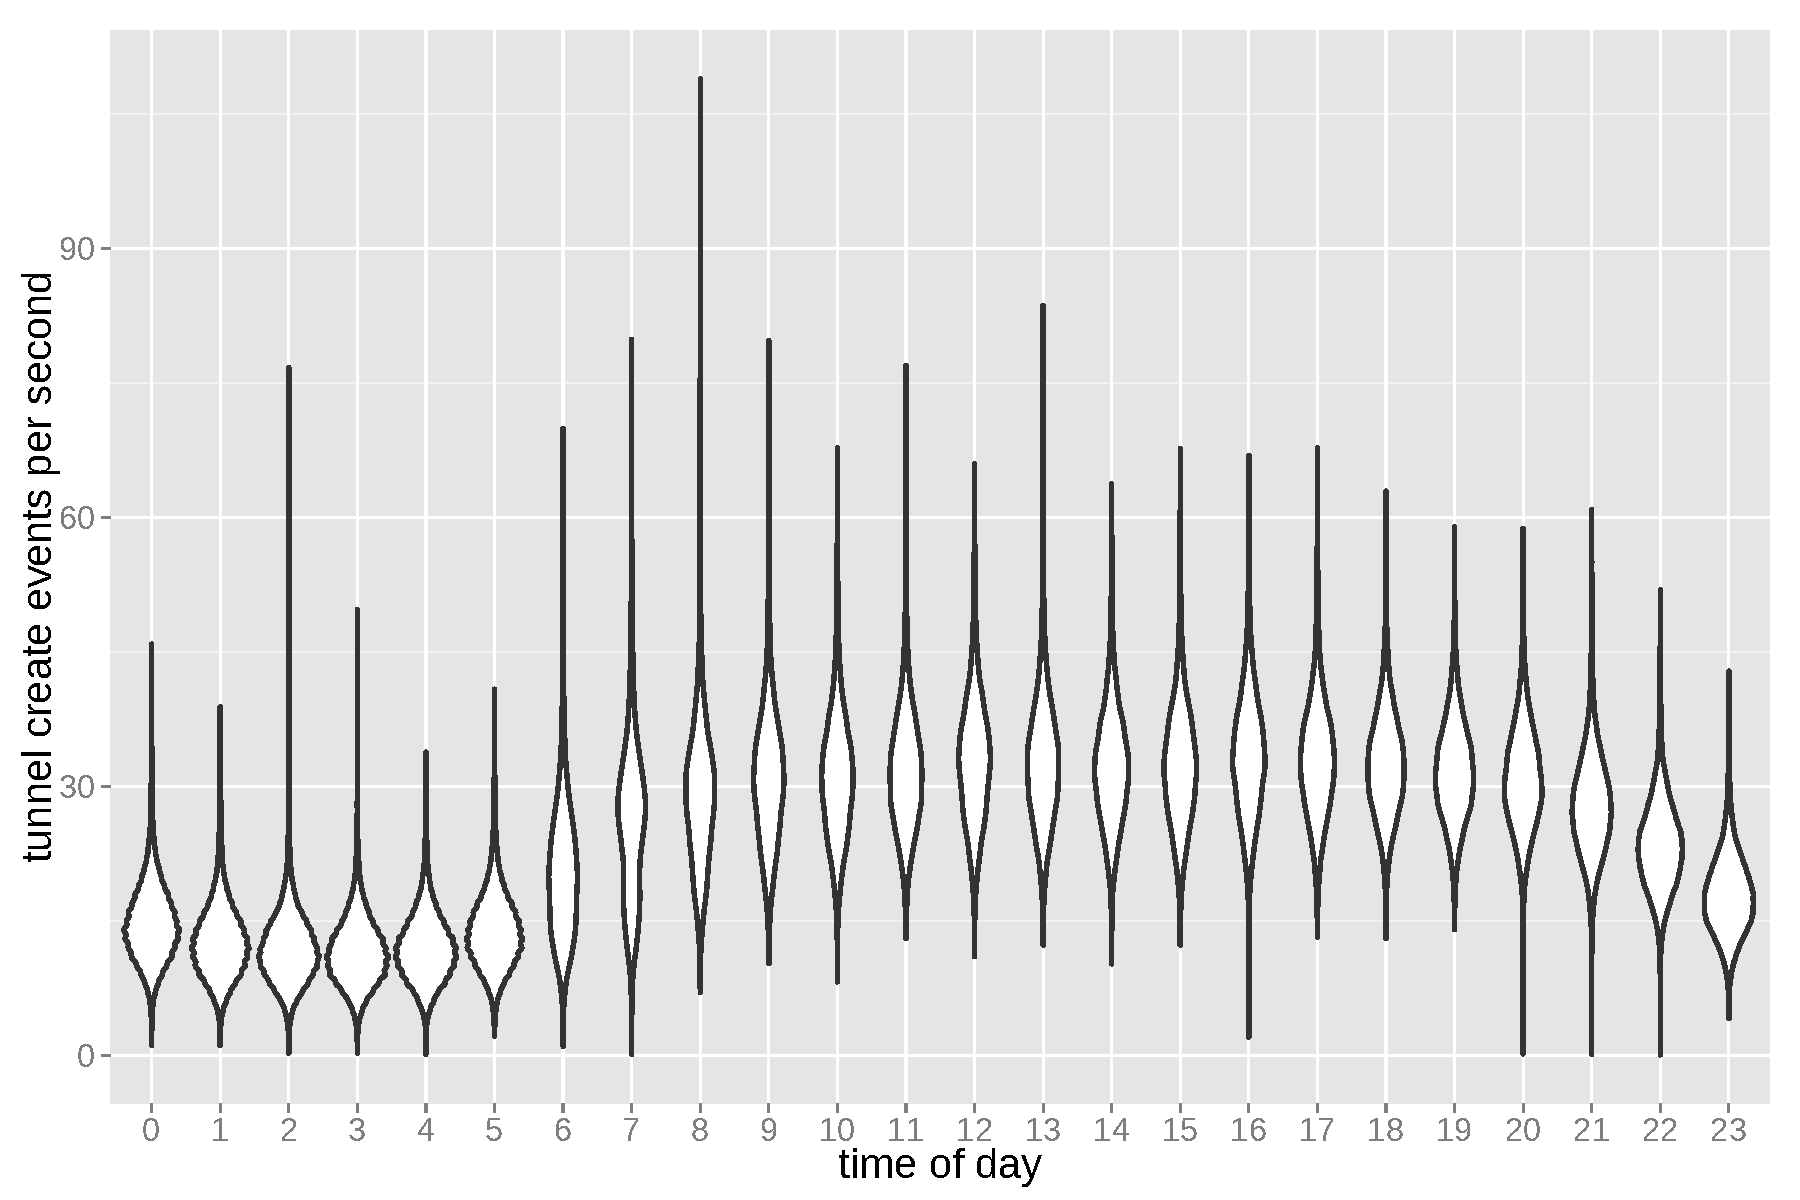
\includegraphics[width=0.9\textwidth]{images/R-createspersecond-1h-violin.pdf}
	\caption{Violin plot of tunnel arrivals in one second per time of day.}
\label{c4:fig:freq-arrivals-per-second-violin}
\end{figure}

A reasonable cause for the occurrence of these two modes can be found in the diurnal arrival patterns. Figure~\ref{c4:fig:freq-arrivals-per-second-violin} contains a violin plot of the tunnel arrivals. This type of plot is similar to a box plot but additionally shows the density of the individual items on the vertical axis. Here the arrivals are broken down to hourly slots. 

The nocturnal plateau of arrivals between midnight and \formattime{5}{0}{0} and the longer daytime plateau between \formattime{8}{0}{0} and \formattime{19}{0}{0} match the two modes found in the histogram. In between are short transition phases. The density of the arrivals during daytime indicates a spread of the number of arrivals over a larger range. This could be an indication of load fluctuations in the system.

\begin{figure}[htb]
	\centering
	\begin{subfigure}[b]{0.5\textwidth}    
		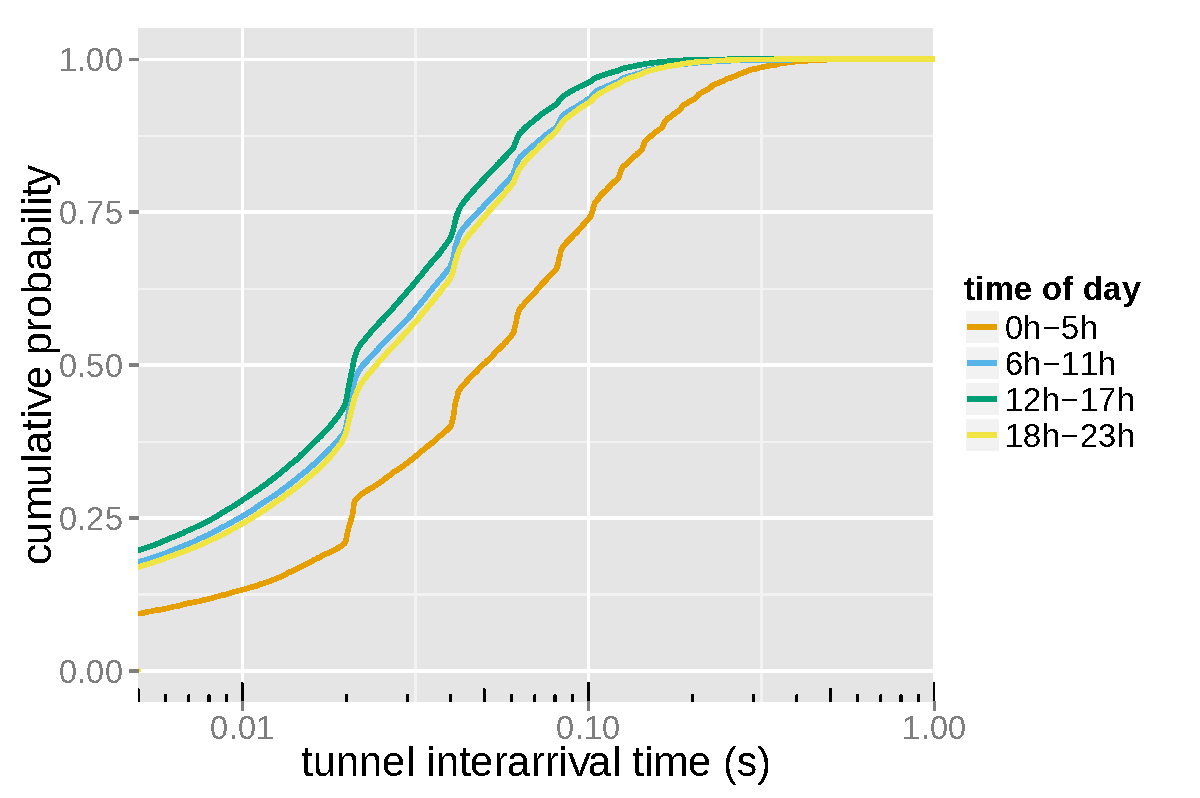
\includegraphics[width=\textwidth]{images/R-IAT-successful-2h-ecdfs.pdf}
		\caption{All tunnel requests.}
		\label{c4:fig:IAT-ecdf-2h-successful}
	\end{subfigure}%
	~
		\begin{subfigure}[b]{0.5\textwidth}
		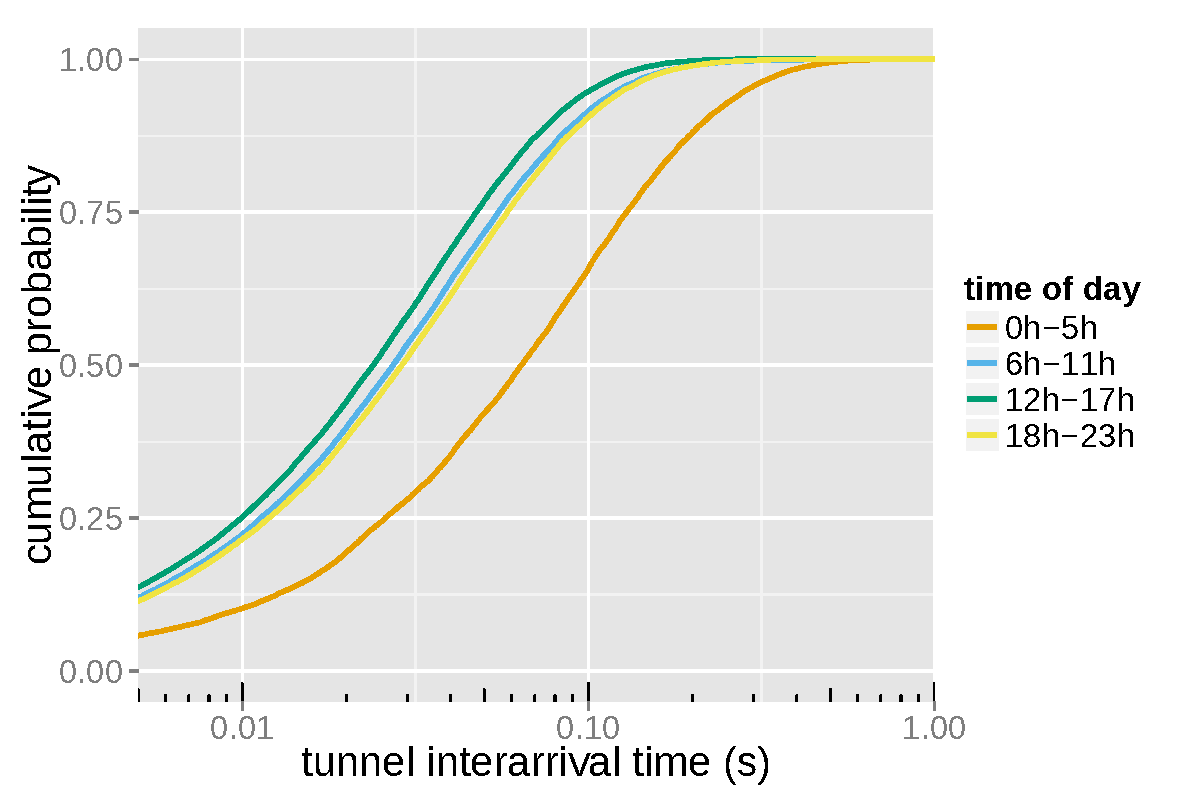
\includegraphics[width=\textwidth]{images/R-IAT-fromflows-ecdfs-2h.pdf}
		\caption{Only tunnels with data flows.}
		\label{c4:fig:IAT-ecdf-2h-active}
	\end{subfigure}

	\begin{subfigure}[b]{0.5\textwidth}
		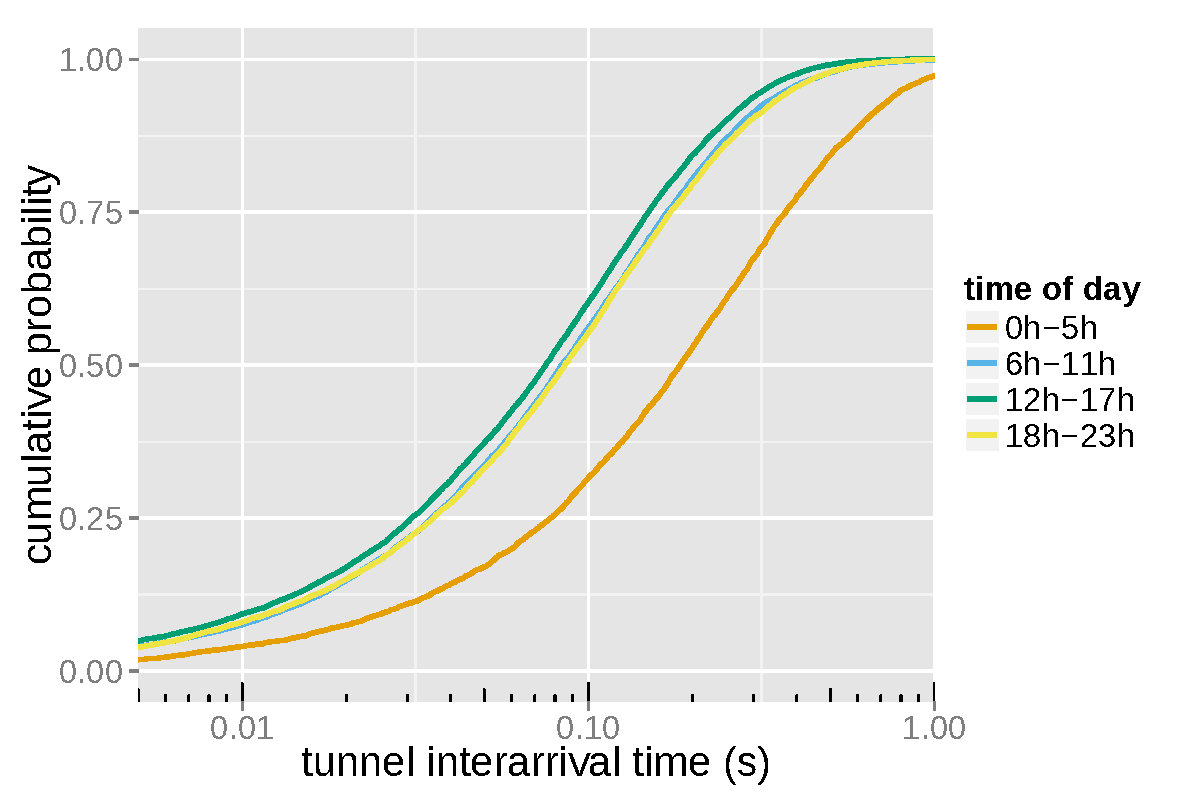
\includegraphics[width=\textwidth]{images/R-IAT-fromflows-gprs-ecdfs-2h.pdf}
		\caption{Tunnels with data flows initiated in \gls{GPRS}.}
		\label{c4:fig:IAT-ecdf-2h-active-gprs}
	\end{subfigure}%
	~
	\begin{subfigure}[b]{0.5\textwidth}
		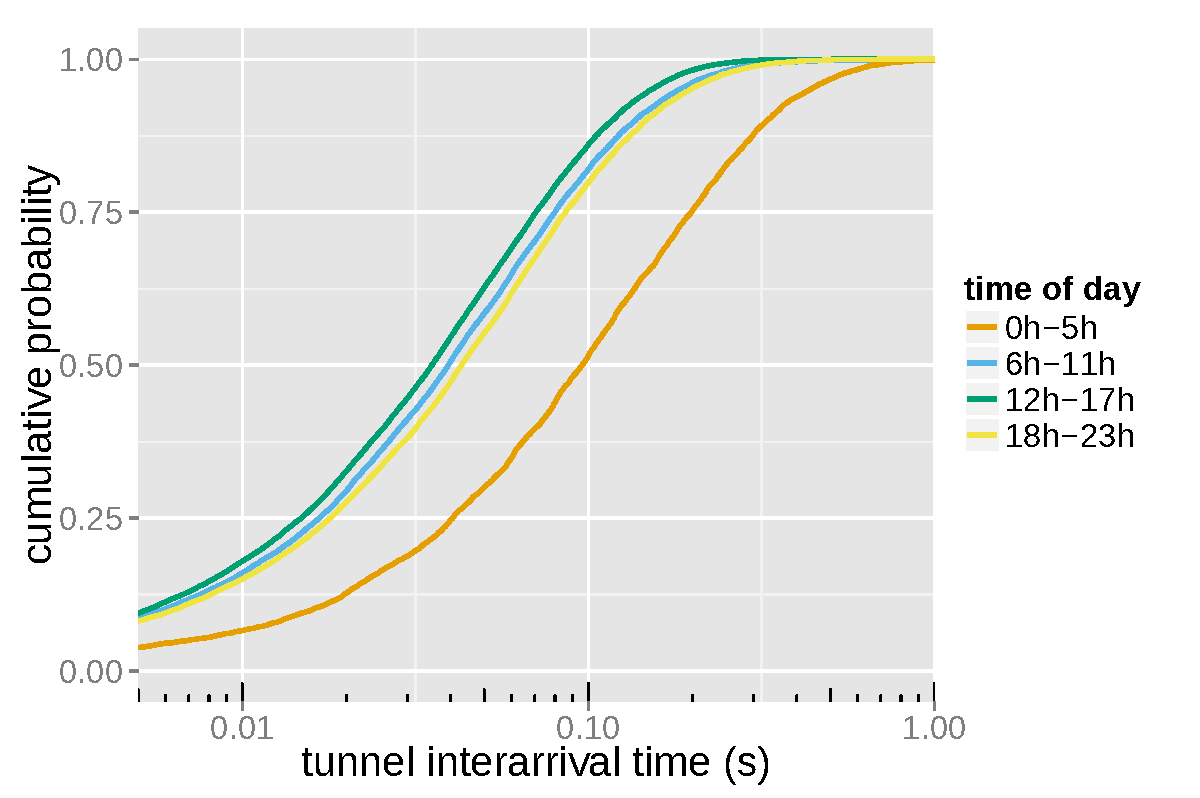
\includegraphics[width=\textwidth]{images/R-IAT-fromflows-umts-ecdfs-2h.pdf}
		\caption{Tunnels with data flows initiated in \gls{UMTS}.}
		\label{c4:fig:IAT-ecdf-2h-active-umts}
	\end{subfigure}
	\caption{\acrshortpl{ECDF} of the tunnel \acrshort{IAT} in seconds by time of day.}
\label{c4:fig:IAT-ecdf-2h}
\end{figure}

Complementing the arrival rate evaluation is the investigation of the tunnel \gls{IAT}. This metric is more sensitive to short time fluctuations of arrivals and more suited to describe the arrival process for use in the proposed load model.

The overall picture of all arrivals is given in the \gls{ECDF} of Figure~\ref{c4:fig:IAT-ecdf-2h-successful}, again broken down by time of day. Obviously the the same previously observed diurnal load oscillation can again be perceived. The median \glspl{IAT} fall in the range of \SI{20}{\milli\second} and \SI{60}{\milli\second}, enveloped by the \formattime{16}{0}{0} and \formattime{2}{0}{0}distributions on with the lowest and highest \gls{IAT} respectively. Additionally, tunnel arrivals are occurring at an increased frequency with an interval of multiples of \SI{20}{\milli\second}, which generates these wave-like steps in the \gls{ECDF} plot. As this is happening very regularly at every time of the day, a source inside the mobile network is indicated.

A hypothesis as to the origin of this effect is the value of the \gls{TTI}. This property determines the duration of a mobile network's radio transmission slot. In \gls{3GPP} standards up to \gls{UMTS} the default value of the \gls{TTI} is either \SI{10}{\milli\second} or \SI{20}{\milli\second}, newer versions of the specification set the value to \SI{2}{\milli\second} (in \gls{HSPA}) or even \SI{1}{\milli\second} (for \gls{LTE}). The absolute time of every transmission slot is also synchronized across every base station in the whole mobile network, which makes the \gls{TTI} noticeable even when not measuring directly at the radio link. 

The observed step-width of \SI{20}{\milli\second} therefore indicates that the tunnel establishment signaling procedure includes at least one trip from the mobile device over the radio interface. This makes sense, as the tunnel is typically created during the \gls{GPRS} Attach procedure, which is indeed initiated at the user's device. Unfortunately, this gives the arrival process batch properties. As a result the load at the \gls{GGSN} increases momentarily when a batch arrives. The \gls{GGSN} would then need to process more requests simultaneously than if the arrivals followed a smooth stochastic distribution.

This effect becomes more peculiar when the tunnel arrivals are further broken down. Figure~\ref{c4:fig:IAT-ecdf-2h-active} only displays arrivals of tunnels that actually transported user traffic during their lifetime. Here, the influence of the effect is visually unnoticeable. This could be attributed to the fact that most active data connections during the time of the trace recording were already using almost exclusively \gls{HSPA} or better, which sees the much lower \gls{TTI}. Only older, regular phones establish plain \gls{UMTS} connections and often do not even use it.

The discrimination of the \gls{IAT} distribution by \gls{RAT} that was used during the creation of the tunnel reveals no further information. Due to the much lower number of connections the \gls{GPRS} distributions are shifted to much higher intervals than the \gls{UMTS} specific distributions.


%%%%%%%%%%%%%%%%%%%%%%%%%%%%%%%%%%%%%%%%%%%%%%%%%%%%%%%%%%%%%%%%%%%%%%%%%%%%%%%
\subsection{\texorpdfstring{\acrshort{gtp}}{GTP} Tunnel Message Processing Time}

Finally, the \gls{GGSN}'s processing time of \gls{gtp} tunnel management messages is investigated. Potentially, this can be a direct measure of the load at the node. In times of higher load one would expect a higher processing time of signaling messages.

From the network trace the processing time can be calculated by two timestamps in each record.
As the trace is recorded at the Gn interface these timestamps represent the points in time the \gls{gtp} signaling request and subsequent response pass on the link to and from the the \gls{GGSN}. Therefore, they can also be interpreted as the start and finish of the involved processing at the \gls{GGSN}.

Generally, the processing time of all three message types --- i.e., creates, deletes and updates --- could be calculated. It would be of special interest to know if the setup time of tunnels is influenced by anything, as this is one of the \gls{GGSN}'s most time-sensitive jobs and can impact the time a user has to wait before being able to actually transfer data. Unfortunately, due to unrecoverable issues with the recording of the dataset, the timestamps for both the create and delete messages records were completely unreliable and did not allow for an investigation of the processing time. 

Only \gls{gtp} update messages were unaffected and gave the opportunity for further investigation. The trace contains roughly two orders of magnitude more update messages than either creates or deletes, spread out almost evenly over the whole observation period. Therefore, a node load investigation should still be possible with just the updates messages.

\begin{figure}[htb]
	\centering
	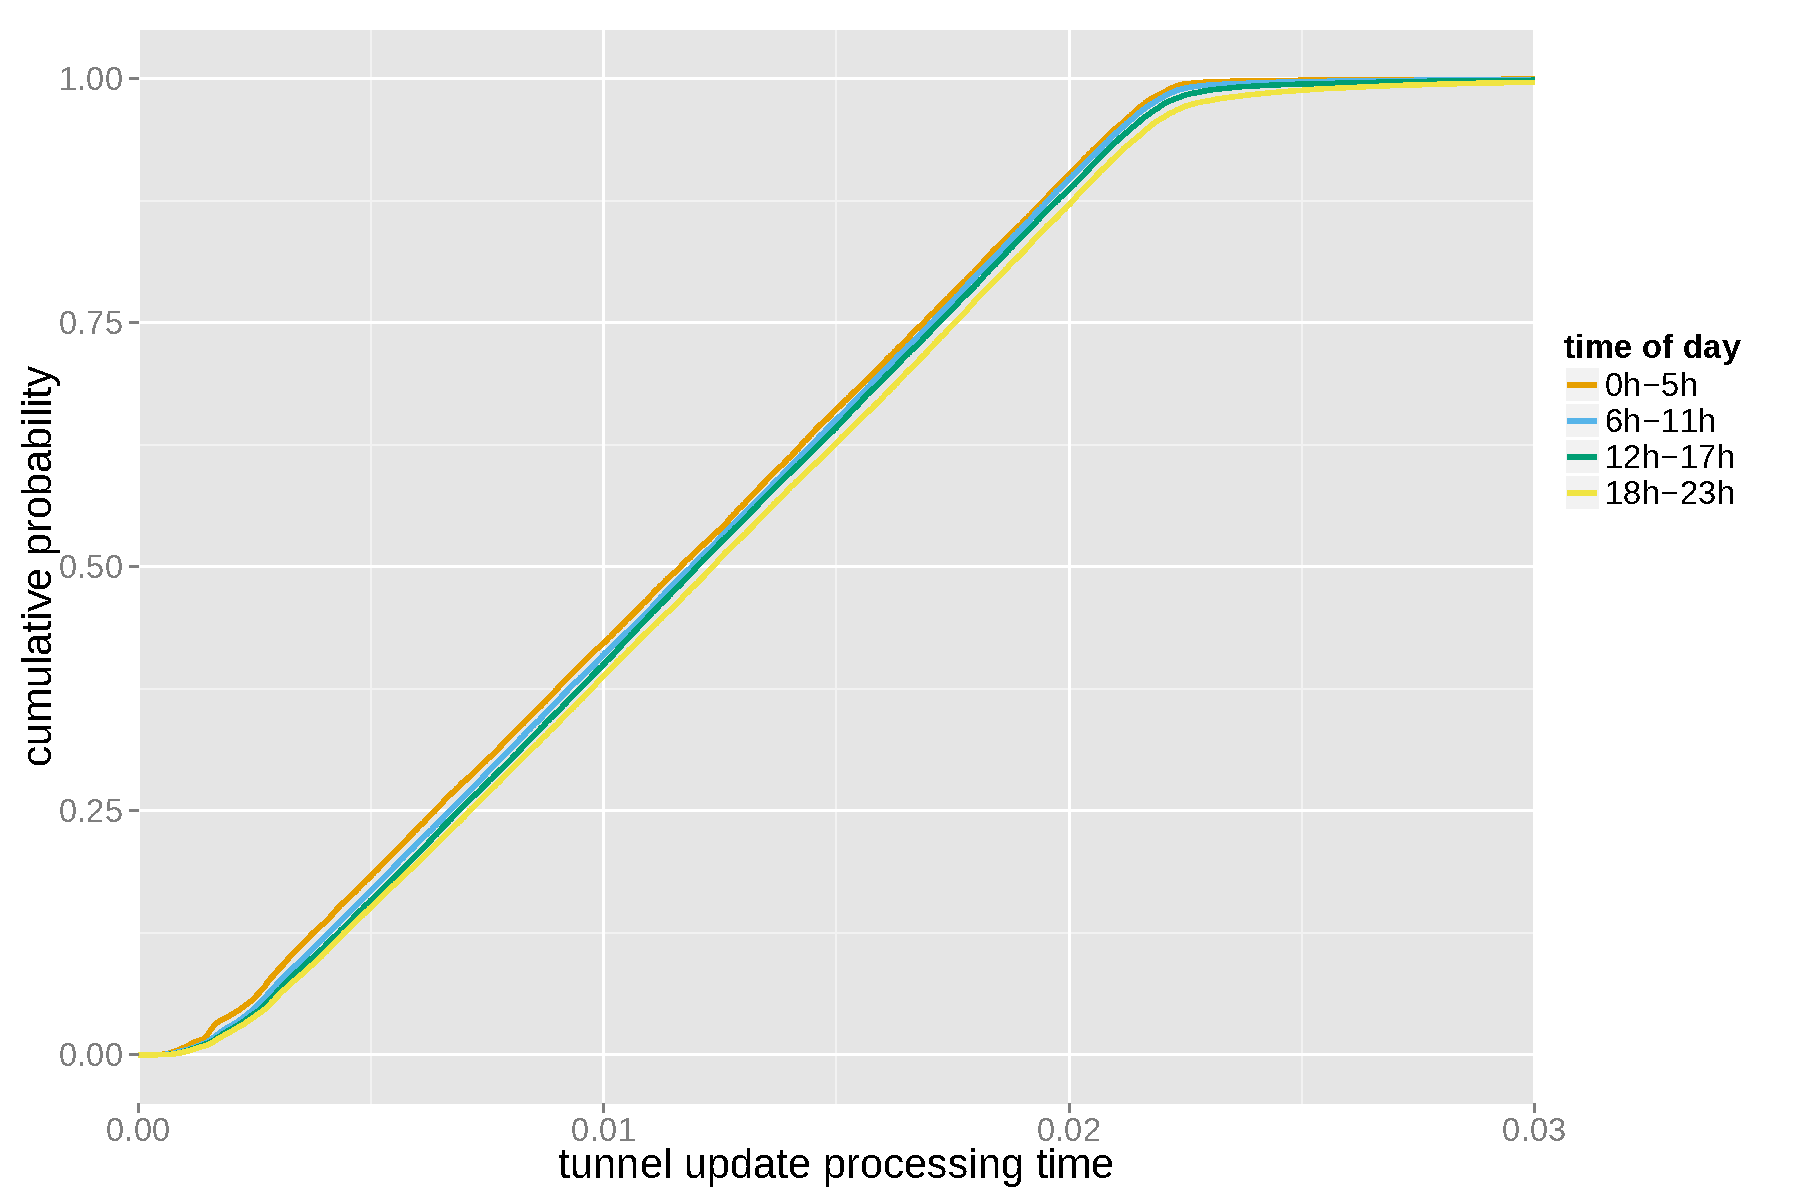
\includegraphics[width=0.9\textwidth]{images/R-update-time-cdfs.pdf}
	\caption{\acrshortpl{ECDF} of the time in seconds it takes a \acrshort{GGSN} to process a \acrshort{gtp} update event, separately plotted for four time slots each day.}
	\label{c4:fig:update-time}
\end{figure}

Figure~\ref{c4:fig:update-time} depicts a band of \glspl{ECDF} for the processing time of update messages by time of day. The processing time distribution almost perfectly follows a continuous uniform distribution between \SI{2}{\milli\second} and \SI{22}{\milli\second}. Only the upper end displays a slight long-tail behavior. The impact of the time of day is very slim with slightly higher processing times during the evening, the same time frame which also experienced an elevated arrival rate.

The occurrence of a continuous uniform distribution is rather unexpected as these do not usually occur in computing processes. According to the central limit theorem one would rather expect to see a normal distribution influenced by, e.g., process scheduling or other queuing artifacts. The source of this effect is still unknown and the current dataset does not allow for a more thorough investigation. Still, the fact that a higher update processing time coincides with an increase in the arrival rate points to an influence of tunnel messaging on the load of a \gls{GGSN}.



%%%%%%%%%%%%%%%%%%%%%%%%%%%%%%%%%%%%%%%%%%%%%%%%%%%%%%%%%%%%%%%%%%%%%%%%%%%%%%%
\subsection{Statistical Evaluation and Data Fitting}
\label{c4:sec:statistical_evaluation}

The uncovered empirical distributions for both the tunnel duration and the tunnel \gls{IAT} are now to be matched against theoretical probability distributions. Therefore, a univariate distribution fit to the experimental data was conducted. Having a concise representation for the empirical data will help in creating a model of the core network, which is the task conducted in the sections following after this.


%%
\paragraph{\gls{IAT} Fitting}

\begin{figure}[htb]
	\centering
	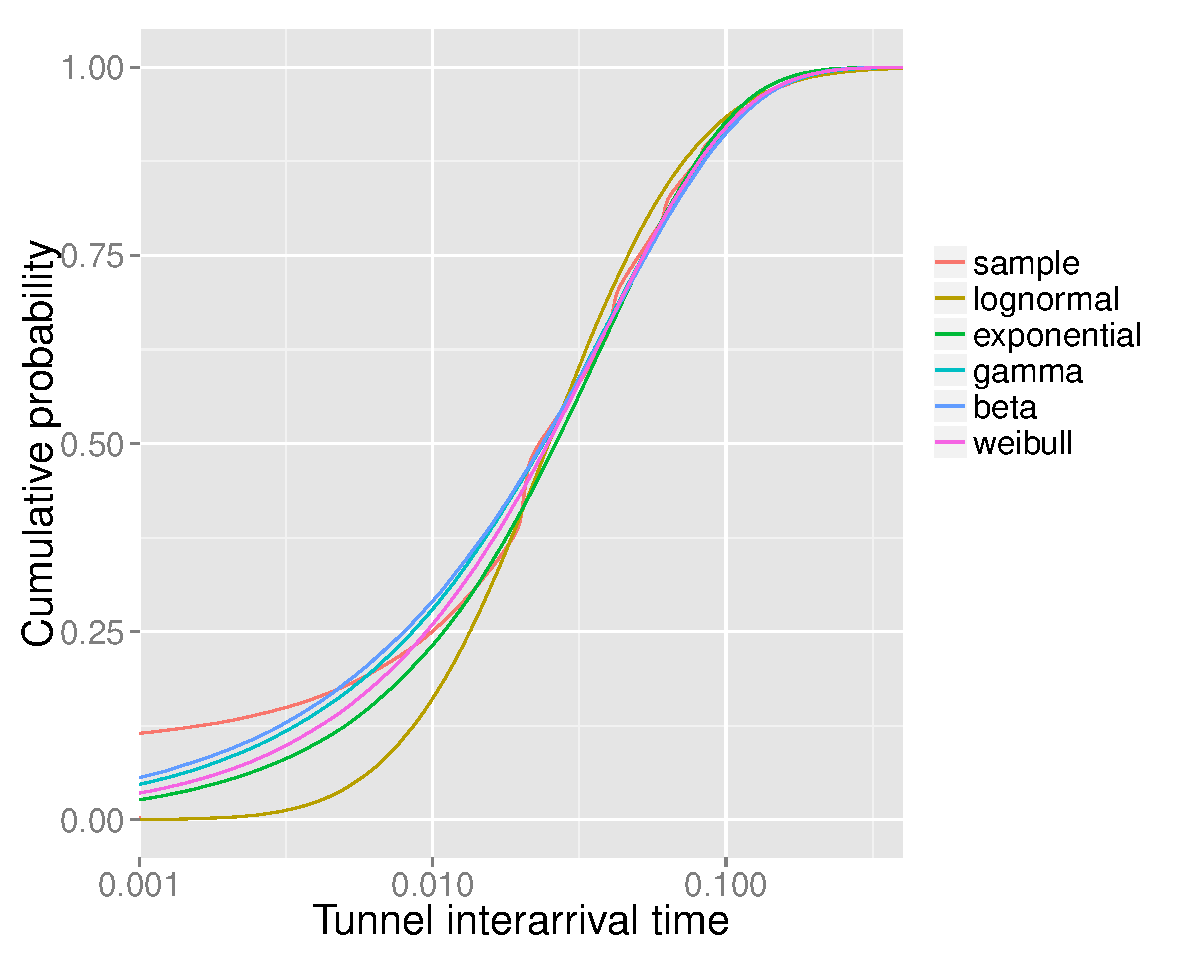
\includegraphics[width=0.9\textwidth]{images/R-IAT-ecdfs.pdf}
	\caption{Sampled inter-arrival time \acrshort{CDF} and fitted theoretical distributions.}
\label{c4:fig:IAT-cdfs}
\end{figure}

In order to investigate the tunnel \gls{IAT}, Figure~\ref{c4:fig:IAT-cdfs} displays the overall \gls{ECDF} with fits for various basic probability distributions. Each of the fits was generated through the method of moments matching.

The goodness of these fits was checked both visually using the \glspl{CDF} plots and numerically with goodness of fit measures, using Pearson's correlation coefficient and Pearson's $\chi^2$ test. Unfortunately, none of the probability distributions reaches the significance level for $\chi^2$. This can probably be largely attributed to the various previously described artifacts in the data. Matching them visually, the exponential fit seems to be reasonably close to the experimental data.

\begin{figure}[htb]
	\centering
	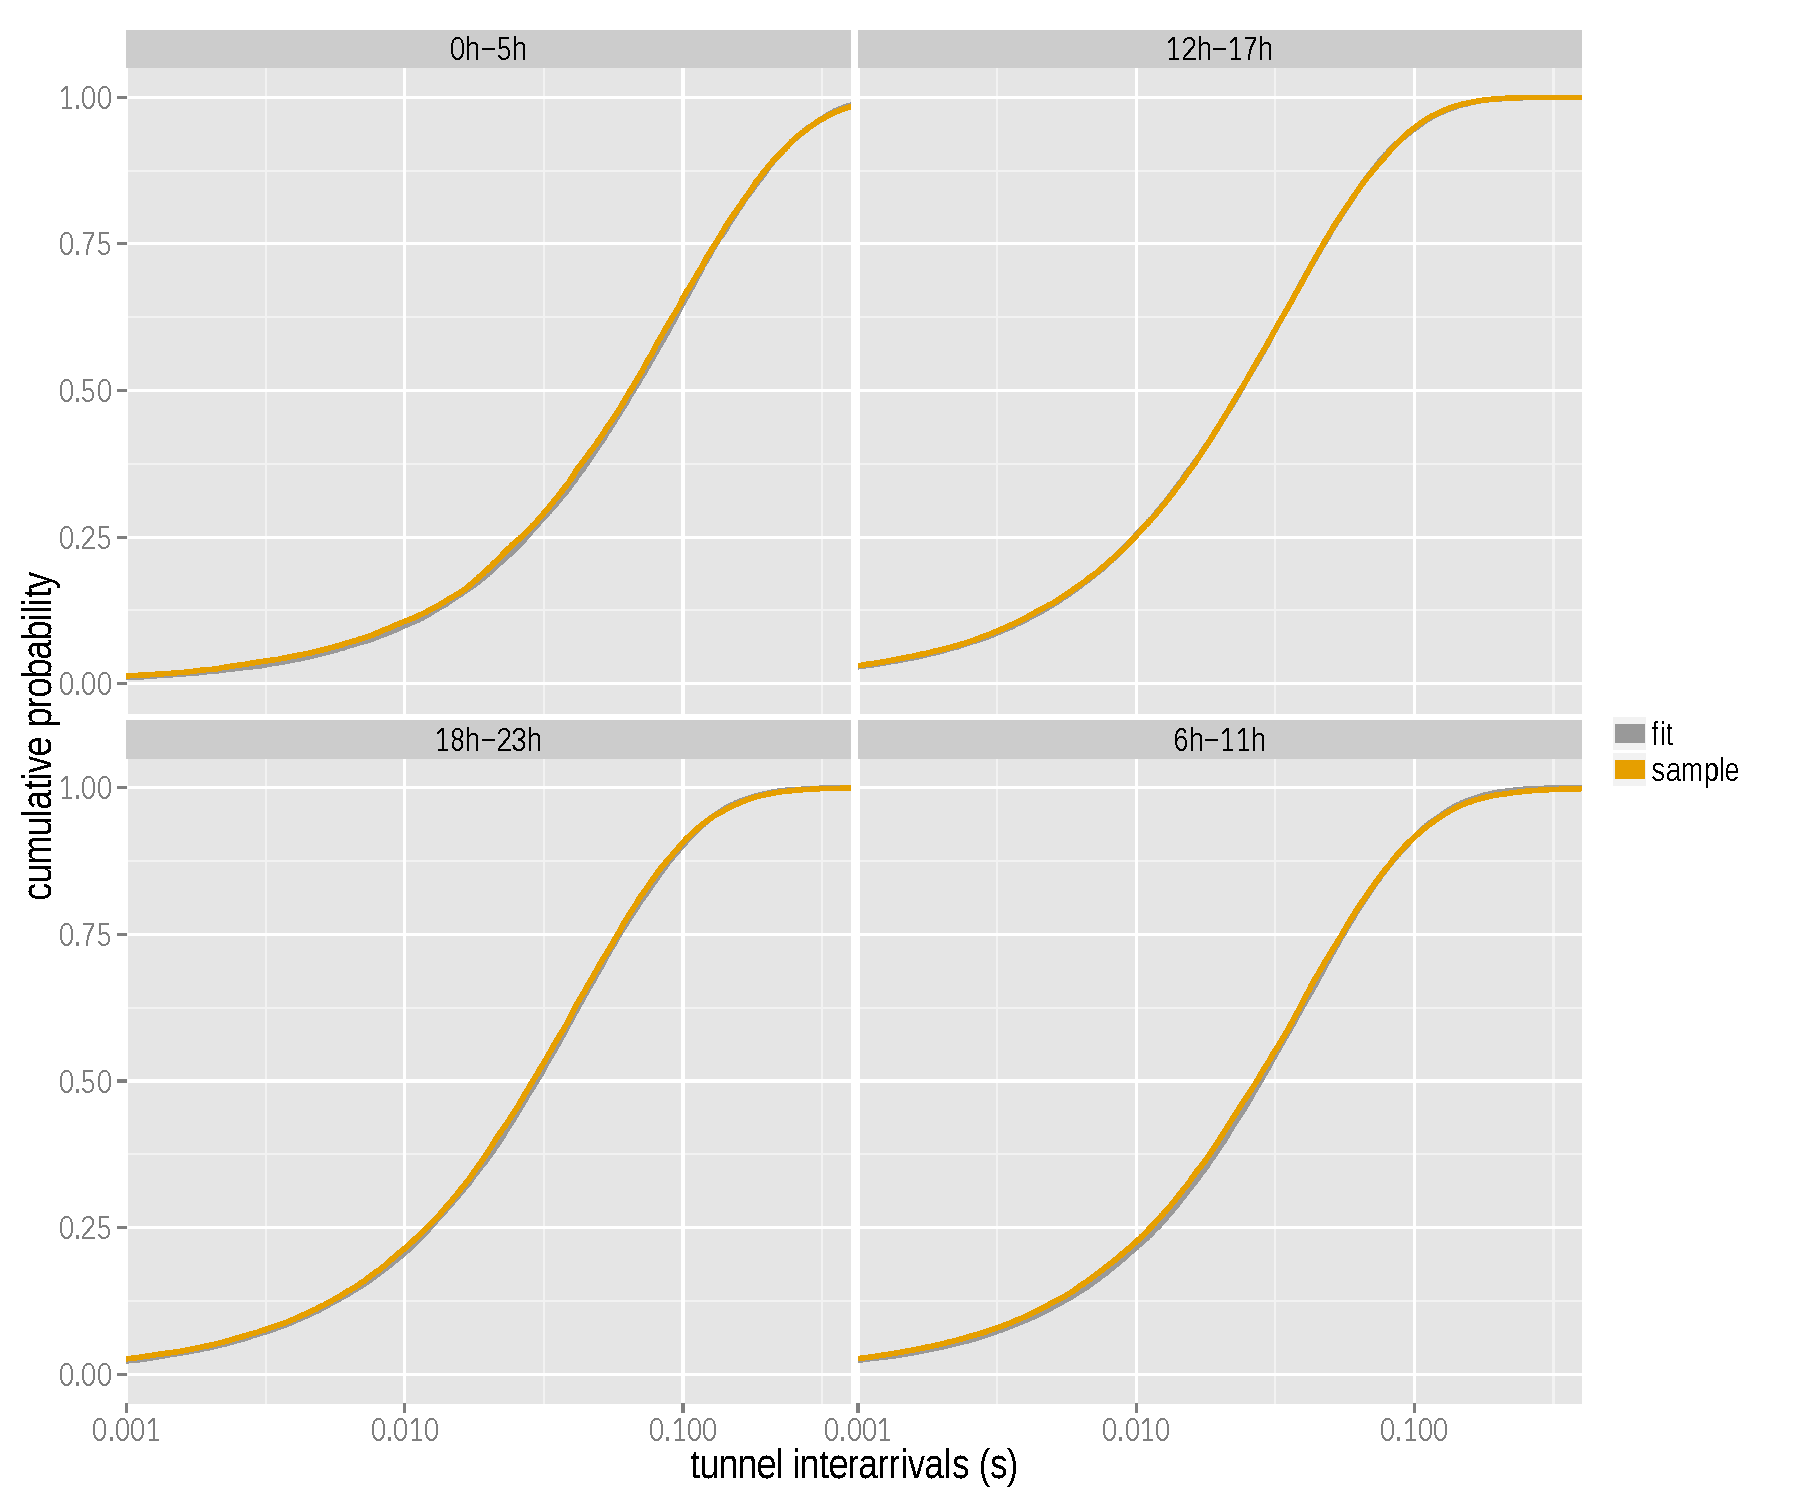
\includegraphics[width=0.9\textwidth]{images/R-IAT-active-fit-cdf-facets.pdf}
	\caption{Empirical and exponentially fitted \acrshortpl{CDF} of the tunnel \acrshort{IAT} by time of day. \acrshortpl{CDF} are overlapping as the coefficient of determination is close to $1$.}
\label{c4:fig:pdparrivalsecdf}
\end{figure}

To improve the fits, two modifications were made to the process. First, to remove the \SI{20}{\milli\second} steps, only the active tunnels were taken into consideration. Second, the overall \gls{IAT} distribution was once again split up into time of day slots. The overall distribution is just a superimposition of the individual slots anyway. Therefore, this should further improve the fidelity of the fits.

\begin{table}[htb]
\caption{Parameters for the exponentially distributed inter-arrival times and corresponding Pearson correlation coefficients.}
\label{c4:tab:IAT-fits}
	\centering
	\begin{tabu}{X[0.9,l]X[r]X[r]} 
	\toprule
	\textbf{Time of Day} & $\mathbf{\lambda}$ & $\mathbf{R_{arrival}}$\\ 
	\midrule
	0h-5h   & $10.67477$ & $0.995$ \\
	6h-11h  & $24.53298$ & $0.992$ \\
	12h-17h & $29.2504$  & $0.993$ \\
	18h-23h & $23.49983$ & $0.986$ \\
	\bottomrule
	\end{tabu}
\end{table}

The results are depicted in Figure~\ref{c4:fig:pdparrivalsecdf}. To improve plot visibility only four larger time slots are displayed here while the actual fits were conducted for each hour slot. Parameters for the exponential distribution $F(x) = 1- e^{-\lambda x}, x \geq 0$ and the corresponding correlation coefficients to the original data for the four time slots are given in Table~\ref{c4:tab:IAT-fits}. The fitted functions match the empirical data quite well, with some deviation present at the left tail but an overall positive correlation coefficient approaching $1$.


%%
\paragraph{Duration Fitting}

The second fitting effort surrounds the empirical data concerning the tunnel durations. However, none of the basic probability distributions (including exponential, gamma, and Weibull distributions) fit the tunnel duration even remotely. One of the reasons for this is probably that the tunnel duration is influenced by an overwhelming amount of factors, which were previously described. This superposition, especially with the user behavior, will result in unpredictable results that does not follow any basic probability distribution.

\begin{figure}[htb]
	\centering
	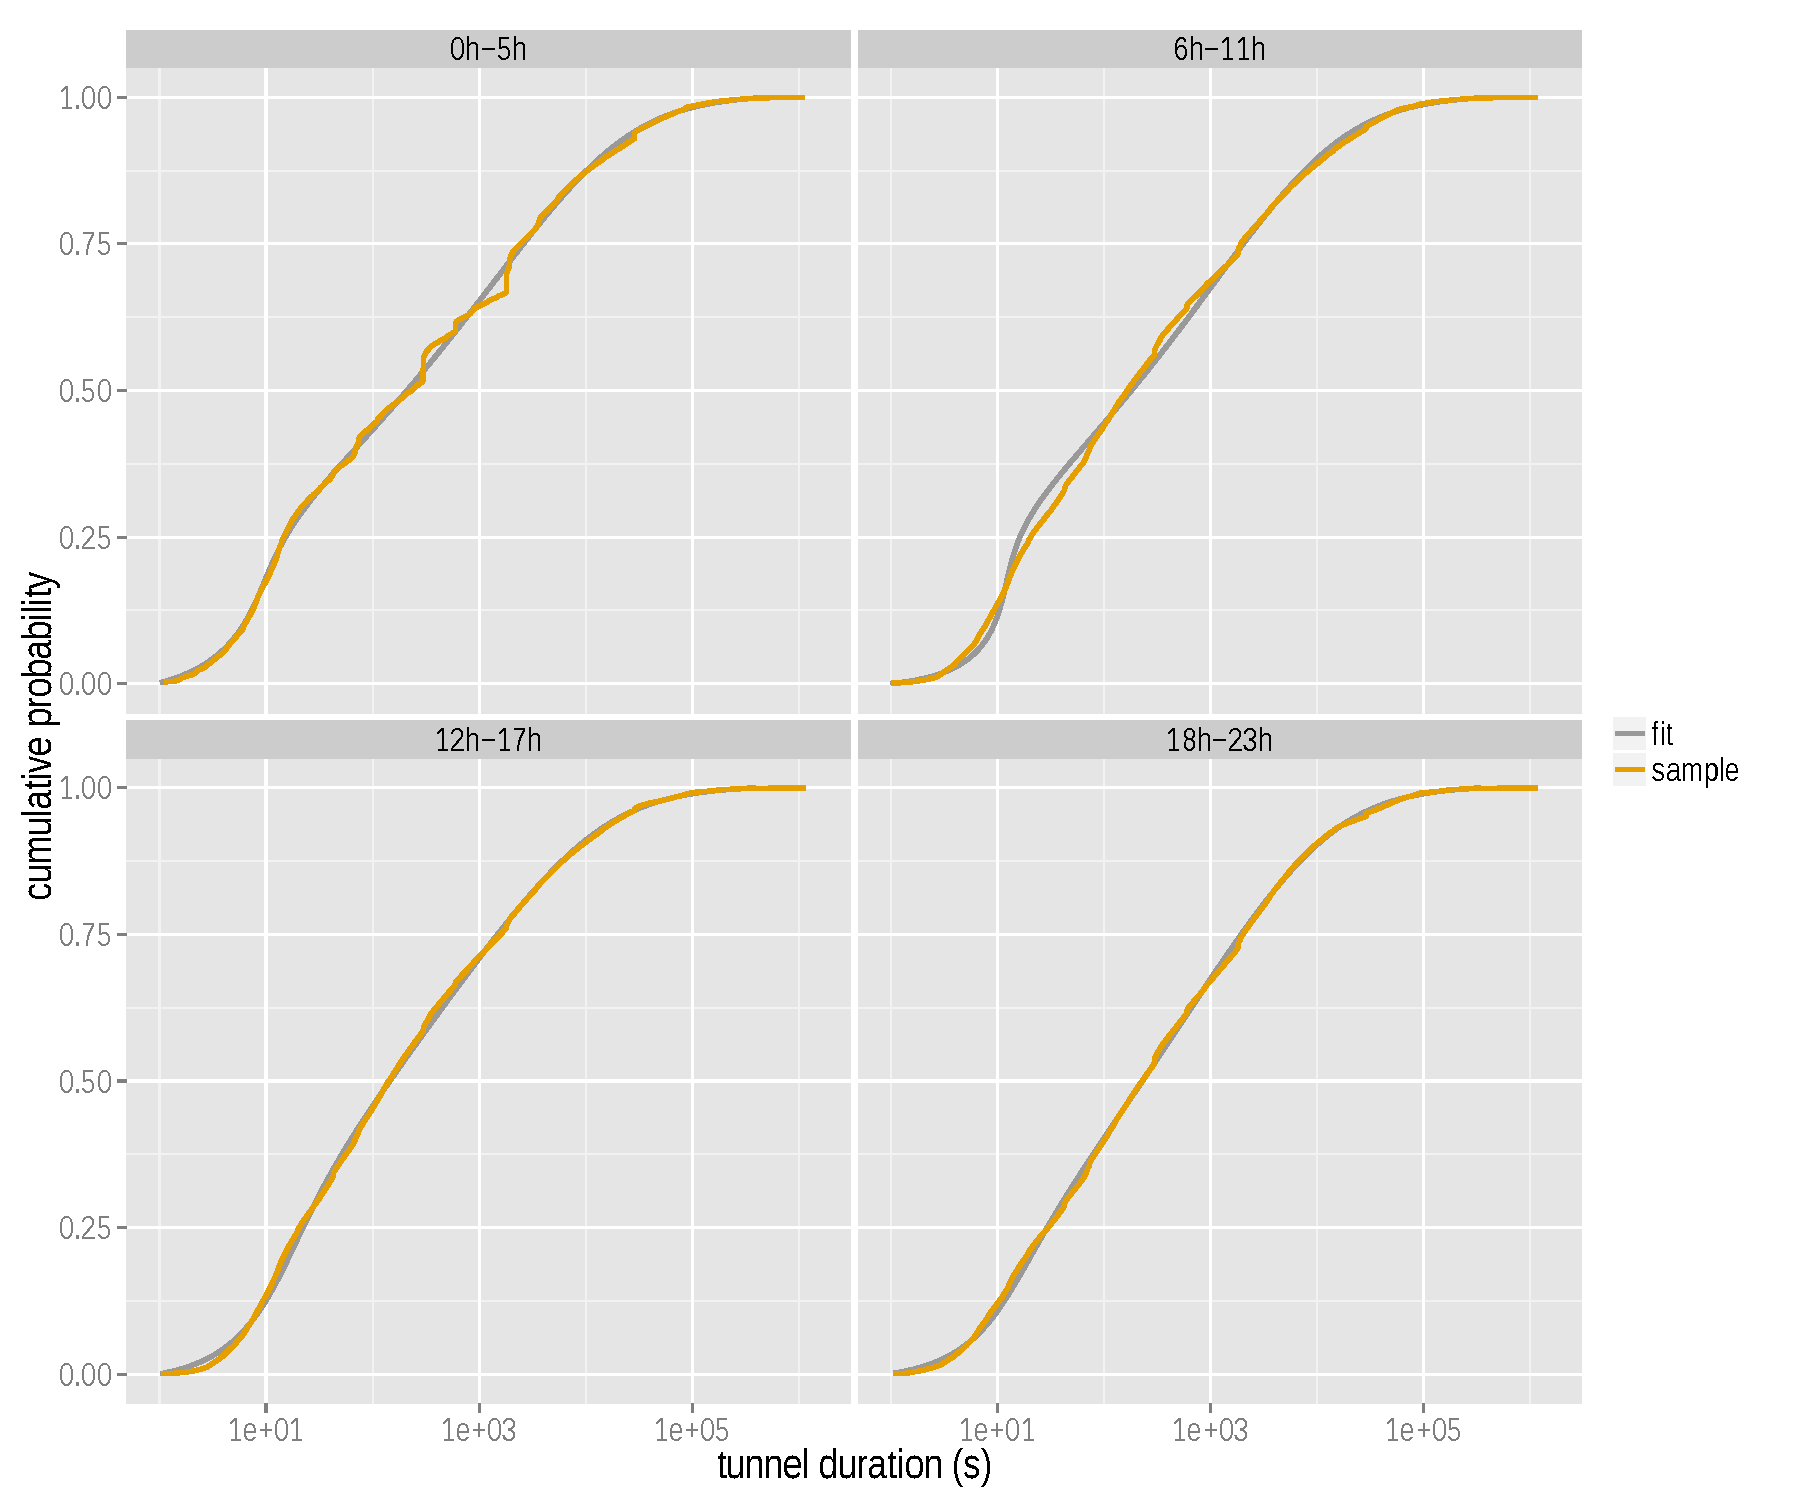
\includegraphics[width=0.9\textwidth]{images/R-duration-fit-cdf-facets.pdf}
	\caption{Empirical and fitted \acrshortpl{CDF} of the tunnel duration by time of day with fitted rational functions.}
\label{c4:fig:fittedsdurationlots}
\end{figure}

Instead, rational functions are fitted to the \glspl{ECDF} using the proprietary third-party tool \textit{Eureqa}~\cite{eureqa_paper, eureqa_software}. This allows for a much closer fit as seen in Figure~\ref{c4:fig:fittedsdurationlots}, but limits its application in the statistical evaluation.

\begin{table}[htb]
\caption{Inverse rational functions fitted to the \acrshortpl{ECDF} of the tunnel duration by time of day and correlation coefficients of the fit.}
\label{c4:tab:fits-duration}
	\centering
	\begin{tabu}{X[1.1,l]X[4.5,r]X[r]} 
	\toprule
	\textbf{Time of Day} & \textbf{Inverse Serving Time \gls{CDF} Representation} & $\mathbf{R_{dur}}$\\ 
	\midrule
	0h-5h & $0.919 - 60.614y - 3498.78y^3 - \frac{110.707y + 2289.94y^3}{y - 1.005}$ &  $0.999$ \\
	6h-11h & $1 + 117.484y - 368.643y^2 - \frac{1720.13y^4}{y - 1.004}$ & $0.999$ \\
	12h-17h & $0.953 + 69.491y + \frac{81146.1y^3 + 1.086\times10^6y^5}{805 - 802.01y}$ & $0.999$ \\
	18h-23h & $0.912 + 82.056y - \frac{2936.93y^4}{1.945y - 1.953}$ & $0.999$ \\
	\bottomrule
	\end{tabu}
\end{table}

	% high precision:
	% 0h-5h & $0.919208 - 60.6136y - 3498.78y^3 - \frac{110.707y + 2289.94y^3}{y - 1.00469}$ &  $0.999$ \\
	% 6h-11h & $1 + 117.484y - 368.643y^2 - \frac{1720.13y^4}{y - 1.0041}$ & $0.999$ \\
	% 12h-17h & $0.952566 + 69.4907y + \frac{81146.1y^3 + 1.08572\times10^6y^5}{805 - 802.01y}$ & $0.999$ \\
	% 18h-23h & $0.911924 + 82.0562y - \frac{2936.93y^4}{1.94468y - 1.9532}$ & $0.999$ \\

Table~\ref{c4:tab:fits-duration} contains the functions which were fitted to the \textit{inverse} \gls{CDF}. The inverse was chosen here to simplify the modeling and simulation process coming afterwards. The functions can be easily inverted again for other purposes. Both the \glspl{CDF} in the plot as well as the Pearson correlation coefficient, which again approach $1$, confirm the goodness of the fitted functions.


% \begin{table}
% \centering
% \caption{TAC Statistics}
% \begin{tabu}{|X|X|X[1.5]|X|X|X|} \hline
% & \textbf{\# of Flows} & \textbf{Total Traffic (Bytes)} &  \textbf{\# of Tunnels} & \textbf{\# of GTP Signalling Msgs} & \textbf{\# of Distinct IMSIs}\\ \hline
% Total          & 2234659247 & 122758578593993 (112TB)    & 16632094 & 409733865 & 1255293 (all) / 1030895 (with flows) \\ \hline
% In TAC DB      & 2228315260 & 122716712007150 (111.61TB) & 14565430 & 372662108 & 1015891 \\ \hline
% Smartphones    & 459990512  & 15721818747754 (14.30TB)   & 10030734 & 311342846 & 476675  \\ \hline
% Regular phones & 5705832    & 448140315058 (0.41TB)      & 897529   & 3860162   & 116124  \\ \hline
% 3G dongles     & 1487230062 & 92215931895630 (83.87TB)   & 2114756  & 39053819  & 315003  \\ \hline
% Android        & 241973565  & 7953178401958 (7.2TB)      & 2383255  & 177537567 & 175919  \\ \hline
% iOS            & 161408903  & 5481693567152 (5TB)        & 3145384  & 83374590  & 99679   \\ \hline
% Symbian        & 22827418   & 1332996529271 (1.21TB)     & 3520242  & 18479002  & 162790  \\ \hline
% Blackberry OS  &            & 128074907884 (0.12TB)      &          &           &         \\ \hline
% \end{tabu}
% \end{table}


%Devices with GTP signaling but no user plane traffic: (\#distinct imsis gtp db)-(\#distinct imsis flow db):
% $255293-1030895=224398\text{ or }17.88\%$

%%%%%%%%%%%%%%%%%%%%%%%%%%%%%%%%%%%%%%%%%%%%%%%%%%%%%%%%%%%%%%%%%%%%%%%%%%%%%%%%
%\subsection{Correlations to User Traffic}
% TODO, incl. measurements



%%%
% Direct signaling traffic overhead in relation to user traffic and induced network load

% GTP Header: 12 Byte
% IE header and footer: 2 Byte
% Maximum minimum data size including all \glspl{IE}: 221 Byte + 12 Byte Header + 2*37 Extension Header = 307 Byte
% Minimum size of message with just mandatory \glspl{IE}: 12 + 30 + 2*5 = 52 Byte

% 307 Bytes:
% calculation from our dataset
% Total maximum signaling traffic with this calculation: 117.15GB
% Ratio: 0.10\%
% 52 Bytes:
% Total maximum signaling traffic with this calculation: 19.84GB
% Ratio: 0.02\%
% Total traffic: 122758578593993


% signaling calc:
% gtp signaling traffic volume estimation $v_s$ = (1059B gtp message + 8B udp header + 20B ipv4 header) = 1087B * 409733865 number of request/response pairs * 2 (2 messages per pair) = 8,9076142E11B
% ratio to total $r=\frac{v_s}{v_t}=0.72\%$  $v_t=122758578593993B$


%%
%TODO: radio access type plots, if we have the data
% We do not.
%
%\begin{figure}
%\centering
%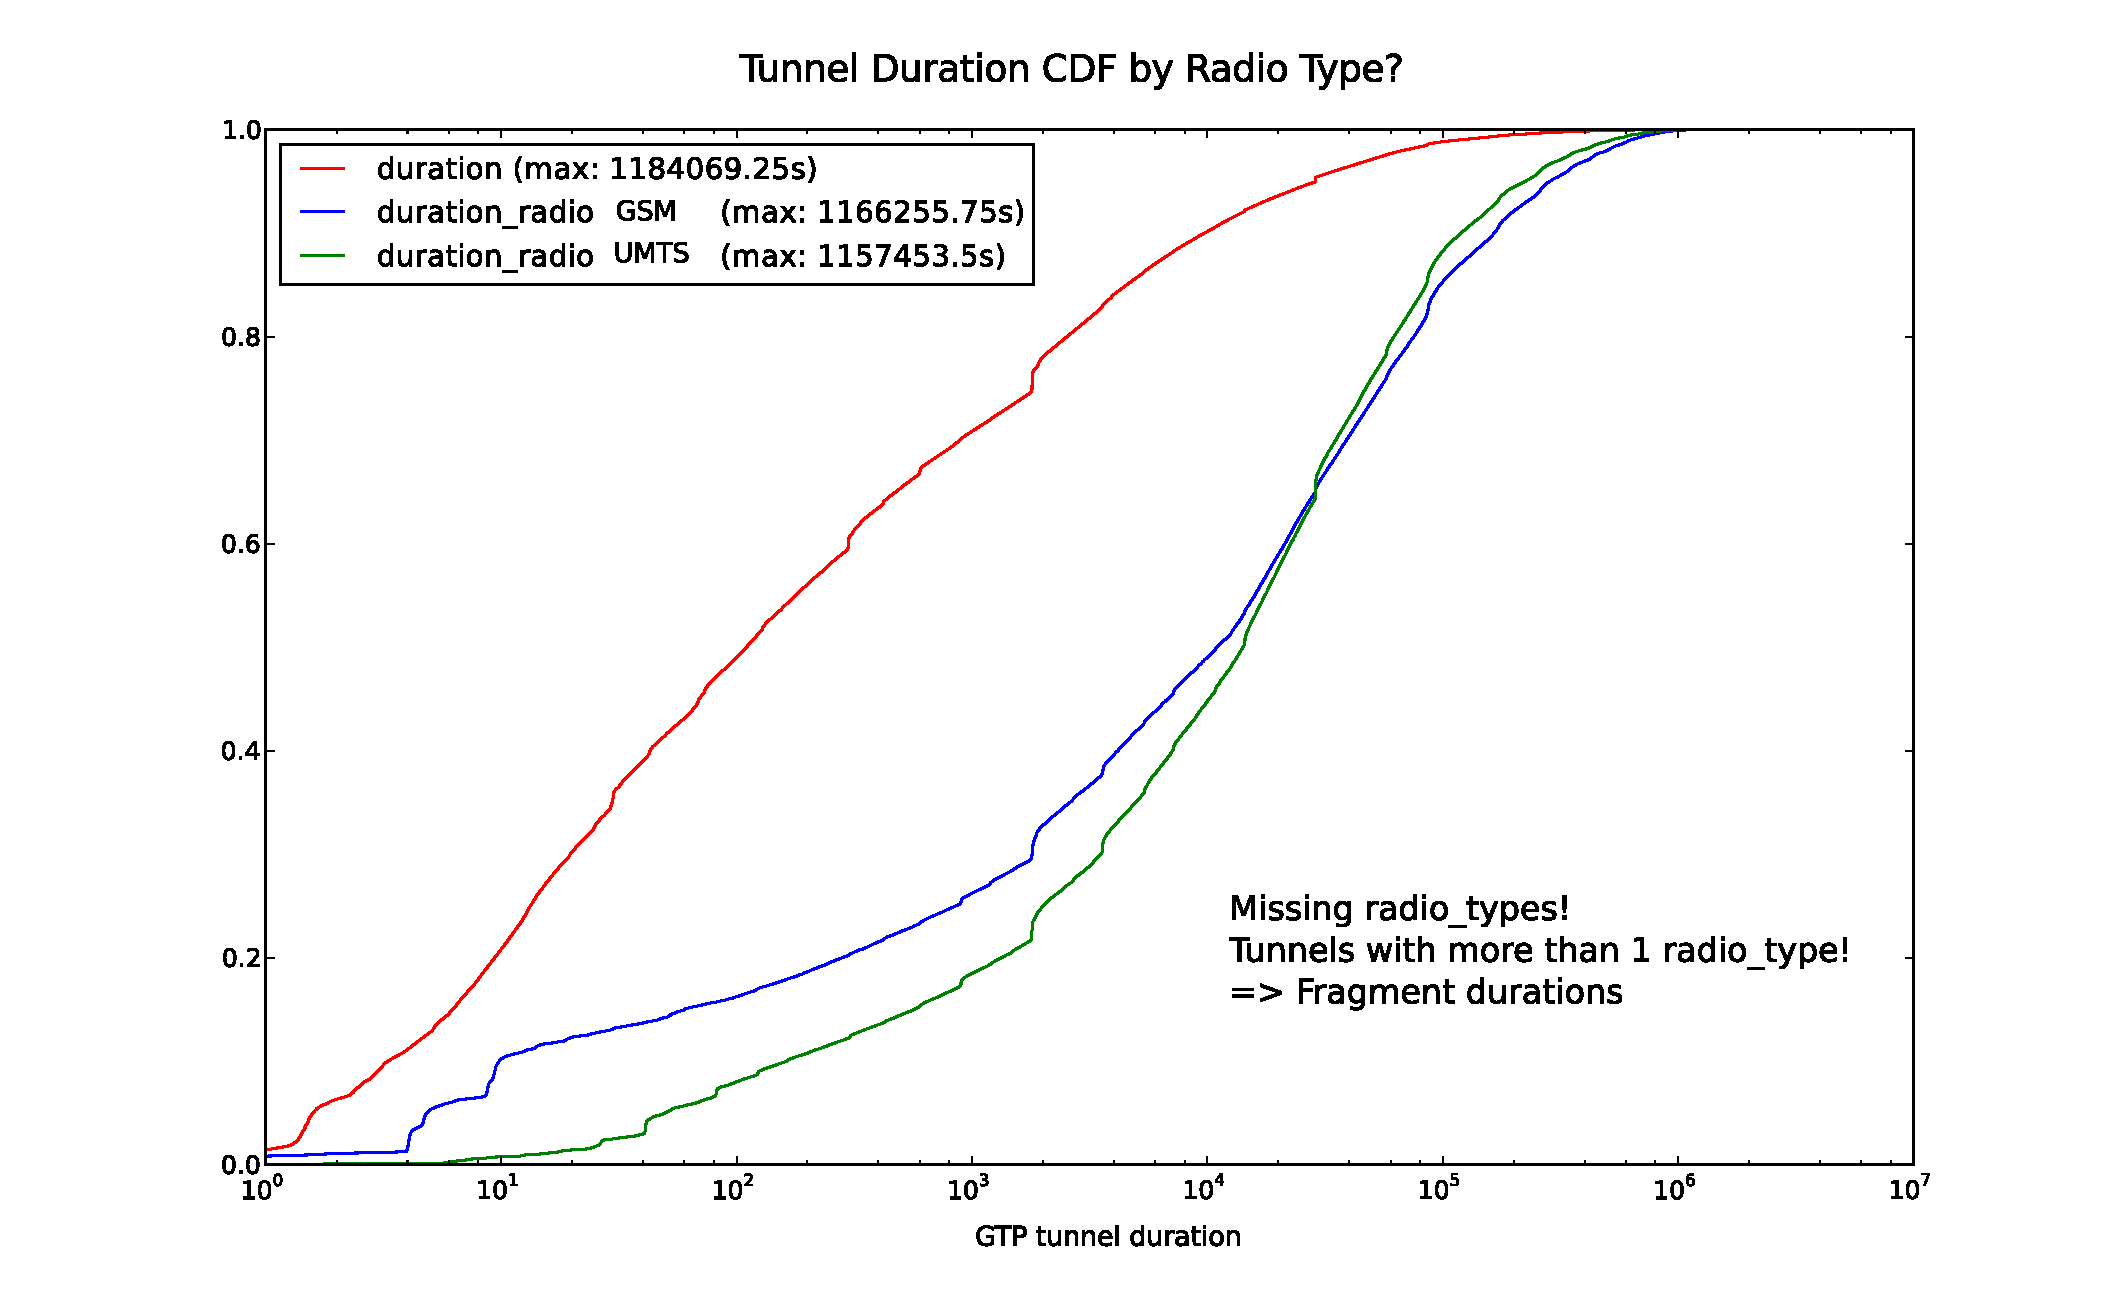
\includegraphics[width=\columnwidth]{figures/tunnel-dur-radio-cdf-mod.pdf}
%\caption{Tunnel duration distribution, separated for UMTS and GPRS radio access [NOTE: only in the last tunnel segment; and majority of radio types %is unknown anyway.}
%\label{fig:cdf-duration-radio}
%\end{figure}



%%%%%%%%%%%%%%%%%%%%%%%%%%%%%%%%%%%%%%%%%%%%%%%%%%%%%%%%%%%%%%%%%%%%%%%%%%%%%%%%
\section{Defining Core Network Load}
\label{c4:sec:loaddefinition}

Before beginning the evaluation, the primary question driving this investigation was: ``How can load in a core network be defined and measured?'' A summary of our thoughts to this question follows here.

With the basics of the architecture in mind, a top candidate for high load is the \ac{GGSN}. All traffic leaving or entering the packet switched domain must go through this element, and it is in control of the described GTP signaling procedures as well. Being an endpoint for the GTP tunnel makes it responsible to sort and encapsulate incoming traffic into the corresponding user tunnel. To accomplish this a lot of state has to be kept -- and processed when signaling occurs. Therefore, our working hypothesis is, that in order to determine load the \ac{GGSN} needs to be monitored closely and any traffic related to this node investigated for indications of the current load.

For our definition of the term ``load'' we differentiate between signaling load and overhead on the one hand and processing load and memory consumption on the other hand. Both are measures of load at specific nodes. While the former mostly has an impact on the actual network traffic, the latter can only be grasped inside the network element. With our data we can directly investigate the signaling traffic but indirect measures for the processing load and memory usage have to be found. In the rest of this section we evaluate the results of several approaches to both of these definitions of load.

While looking at the \ac{GGSN} may be the most obvious choice, it is by far not the only one. 
In addition to GTP tunnels the \ac{SGSN} has to handle \ac{RAB} and mobility management as well. However, it is assumed, that there are more regionally distributed \ac{SGSN} nodes present in a typical mobile network. This means that a single element would have to handle less mobile devices and therefore load. One has also to bear in mind that the \ac{SGSN} can be completely circumvented by setting up a direct tunnel between \ac{GGSN} and \ac{RNC}.

Apart from the two gateways directly inside the traffic path there are several other nodes essential to the control plane decision making, which may very well be also very load-sensitive. The \ac{HLR} for example is a central database storing all user related information which need to be retrieved any time a user needs to undergo initial authentication and authorization. Typically, the procedures the elements are involved in are fewer and they are also harder to investigate with the data available to us. Hence, it was decided to concentrate just on the case of the \ac{GGSN}.


%%%%%%%%%%%%%%%%%%%%%%%%%%%%%%%%%%%%%%%%%%%%%%%%%%%%%%%%%%%%%%%%%%%%%%%%%%%%%%%
\subsection{Load Influencing Factors}

Having described our understanding of core network load we can now move to discuss some of the factors that could influence the load, making them targets for our evaluation.

The first and arguably one of the most important factors are the mobile devices themselves. Specifically, this covers the behavior of the network layer 1 and 2 implementation (sometimes called ``'baseband'') as well as the \ac{OS} and the running applications. The OS and baseband decide when the device should establish a mobile data connection, how long the connection is held, or which mobile technology takes preference. Depending on the access technology, be it \acs{GPRS}, \acs{EDGE}, \acs{UMTS}, \acs{HSPA}, or \acs{HSPA+}, we can expect subtle differences through their specifications, e.g. in the timing of the radio transmission intervals, which could influence our investigation. 

Some specific tunnel duration properties could stem from the \ac{OS}'s IP and transport protocol implementation. For example, TCP timeouts might be configured to different default values causing mobile connections and tunnels to be held either shorter or longer. Also, mobile network firewalls have been found to interfere with transport and application layer timeout and keep-alive or heartbeat mechanisms on mobile devices \cite{sigcomm11middleboxes}.

The actual user-traffic patterns are generated by the applications running atop the OS. An example for how applications can influence network signaling is the aforementioned ``Angry Birds'' with its ad-retrieval strategy causing network traffic and possibly signaling in certain intervals. Since the application ecosystem for smartphones is extremely rich and ever growing we cannot pinpoint individual ones from our aggregate dataset.

An additional factor in the picture is the user and her or his behavioral patterns. They express themselves both in the traffic dynamics and in the mobility pattern, but they are rather difficult to distinguish in such a dataset given the large amount of data and the difficulty of correctly correlating tunnel management messages. We leave this as potential future work.

Easier to observe are the temporal effects of user behavior, which do not target individual users but the overall effects of a device's usage based on the time of day, the day of the week, or other time spans. In network user traffic analyses diurnal effects are typically very distinct with peak traffic some time during the day and the lowest traffic shortly after midnight. But these investigations are for user traffic only. We aim to find out, if the mobile network control plane shows similar patterns and can thusly be correlated to user traffic.

We also expect the mobile network and its protocol implementations to express themselves in the measurements. For example, the \ac{RRC} idle timer is typically in the range of 10 to 30 minutes, which could mean there will be a large number of tunnels with a duration in this range. Such choices are usually made either by the mobile network operator or the device manufacturer and can vary from one implementation to another. It is therefore quite difficult to give any hard numbers in advance, and one has to correlate such aspects with certain events in the results.




%%%%%%%%%%%%%%%%%%%%%%%%%%%%%%%%%%%%%%%%%%%%%%%%%%%%%%%%%%%%%%%%%%%%%%%%%%%%%%%%
%!TEX root = ../../dissertation.tex
%%%%%%%%%%%%%%%%%%%%%%%%%%%%%%%%%%%%%%%%%%%%%%%%%%%%%%%%%%%%%%%%%%%%%%%%%%%%%%%%
\section{Streaming Modeling}
\label{c3:sec:modeling}

As stated, the goal of this chapter is to model the measuring process and reliable streaming. This section will introduce our reliable \gls{TCP}-based streaming model. It is intended for easily comparing different protocol variants against each other and measuring all variants in one testbed. 

But first, because any evaluation of a model requires metrics, we describe ones appropriate to the model and give a rationale.
 
%%%%%%%%%%%%%%%%%%%%%%%%%%%%%%%%%%%%%%%%%%%%%%%%%%%%%%%%%%%%%%%%%%%%%%%%%%%%%%%%
\subsection{Metrics for Reliable Transport Streaming}
\label{c3:metrics}

When measuring anything related to video or even just image quality, one has the choice between conducting a subjective or objective assessment. 

During a subjective test, human assessors evaluate and rate video quality in a controlled environment with the results usually being aggregated into an overall relative quality score \gls{MOS}. Through the human element, conducting a subjective assessment is very time and resource consuming but it also achieves the highest precision.

This is where, objective video quality assessments come into play. Modern objective models attempt to recreate the features of the humans' visual perception and psychophysics and are calibrated by subjective assessments. Most objective models operate on a full reference approach, they directly compare the original reference video to the resulting video after being encoding or transmitted.

Two of the simplest full reference image quality metrics, which can also be applied on video, are the \gls{MSE} and \gls{PSNR}, defined as:

\begin{equation}
    \begin{aligned}
    MSE = \frac{1}{N} \sum_{i=1}^{N}(x_i - y_i)^2\\
    \text{and } PSNR = 10 \log_{10} \frac{L^2}{MSE},
    \end{aligned}
\end{equation}

with $N$ as the number of pixels in a frame and individual pixels $x$ and $y$ from the reference and output frame respectively. $L$ denotes the maximum value of a pixel. For grayscale or when investigating each color channel separately, usually $L = \SI{8}{\bit} = 255$.  \cite{objective-vqa}

Image quality models can by nature only test for spatial distortions of a single image. This includes a general blockiness or blurriness, noise, or reduced resolution. Dedicated video quality assessments can additionally take temporal metrics into account, e.g. frame rate anomalies. Such models are being researched and standardized by the \gls{ITU} and \gls{VQEG} for example in \cite{ituJ144, ituJ246, ituJ247}.


When conducting dedicated streaming quality measurements, only this portion should be taken into account by a metric, and not the initial encoding process. During streaming only a specific subset of quality degradations can occur. Lost or late packets can cause missing blocks in a frame or frames to be skipped completely. Initial thoughts concerning \gls{IPTV} \gls{QoE} have been given in \cite{ituG1080} and the influence of packet delay variations on playout buffers is investigated in \cite{rfc3393}The \gls{MDI} \cite{rfc4445} is an attempt to capture this behavior and relate it to the network \gls{QoS}. Its metric relies on two properties, the \gls{DF}, as a measure of the network's latency and jitter, and the media loss rate. Of special interest to this investigation is the \gls{DF}, which is calculated based on a virtual buffer (VB) of received stream data as

\begin{equation}
    \begin{aligned}
        VB = r_{rcv} - r_{drain} \\
        DF_i = \frac{\max(VB) - \min(VB)}{r_{drain}}
    \end{aligned}
\end{equation}
 
Reliable streaming has even less possibilities to degrade a video stream. Packets can not be out of order and loss is concealed by \gls{TCP}, meaning that the transmitted and the played video are identical. The only thing that can still happen, is portions of the video arriving too late to be played out at their intended point in time.
A potential reliable streaming quality assessment metric needs to keep track of the following properties:

\begin{itemize}
    \item The initial delay, which is the time delta between the start of the transmission and the start of the video play.
    \item The number and lengths of interruptions or stalls during playback.
    \item For adaptive streaming, the characteristics of the quality levels the video was played in. This includes the number of switching events and the duration of each level.
\end{itemize}

A concise metric covering all properties has not been defined yet. The \gls{CI} was defined in \cite{1498486} and used to determine quality in \gls{P2P} live streaming. It is defined as \enquote{the number of segments that arrive before or on playback deadlines over the total number of segments} and with this partly captures the stalling property. In \cite{5634160} and \cite{DBLP:journals/corr/SeyedebrahimiBP13} a so-called \gls{PI} is defined and evaluated. The definition $I_p = uv$ is simply based on the number of stalls $u$ and the average stall duration $v$. 

Generally, most research operates just directly on these three properties, which allows for the most freedom in usage scenarios. The streaming measurement model presented in the following section also works with the assumption, that only the three properties are of importance. The model assumes no special metric, the individual properties can be directly attained from the model. Though any metric could still be applied on the results.


%%%%%%%%%%%%%%%%%%%%%%%%%%%%%%%%%%%%%%%%%%%%%%%%%%%%%%%%%%%%%%%%%%%%%%%%%%%%%%%%
\subsection{Measurement and Playback Model}
\label{c3:model}

Parts of the model presentation is based on the author's previous work published in \cite{cs3518}, \cite{metzger2011delivery}, and \cite{6229739}. It is based on the desire to compare all in-the-wild variants of reliable streaming protocols in a simple and concise way. This is achieved by basing the model on the component that is common to all of the approaches: the playback buffer.

To display a video stream, an application needs to maintain a playback buffer of sufficient size to at least gather enough data to reconstruct one single atomic unit of playback such as a video frame.
From the perspective of a player application , a video consists of a sequence of atomic units, video frames and audio samples.
The application progressively decodes the video from a source and stores the units temporarily in a memory buffer before playing them. In reliable streaming, the buffer is filled by the payload from received \gls{TCP} segments a subject to the network \gls{QoS}. The process can be subsumed as:

\begin{equation*}
\mathit{buffer}(t) = \sum_{0}^{t} \text{data}_\mathrm{received} - \sum_{0}^{t} \text{data}_\mathrm{played}
\end{equation*}

Both the incoming and outgoing data stream are variable over time. The fill level of the playback buffer is the critical component in the playback process and the central element of the model.If the buffer reaches a size of zero the playback process stops and stalling occurs.

\begin{figure}[htb]
    \centering
    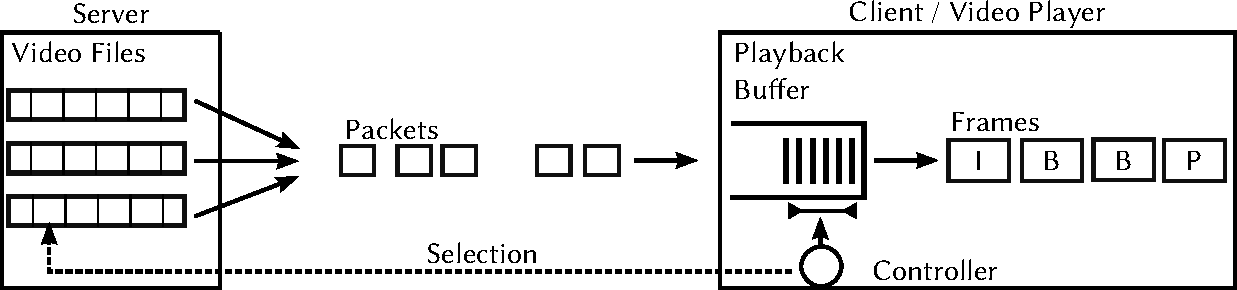
\includegraphics[width=0.9\textwidth]{images/playback-model.pdf}
    \caption{Reliable streaming playback model based on buffer control.}
    \label{c3:fig:playback-model}
\end{figure}

Figure~\ref{c3:fig:playback-model} overviews the reliable streaming model. The controller, part of the video player, selects a video from a remote location and the transmission is started, filling the playback buffer. The model has three degrees of freedom, which are all governed by the controller and together are coined playback strategies. These are:

\begin{itemize}
    \item The initial playback delay, which is the time between the initiation of the video stream transmission and the actual stream playback. The larger this is chosen, the bigger the safety margin on the buffer gets. If the video and transmission bitrate are known to be constant and and appropriately dimensioned, the initial delay can be chosen to be very small.
    \item Playback pause and resume decisions based on the current buffer fill level. This is a generalization of the initial playback delay, which is in fact only one, albeit always occurring stalling period.
    \item Selection of the video or video segment with a video bitrate chosen according to the current network throughput. This is only applicable for adaptive streaming.
\end{itemize}


These decisions yield a stalling period distribution for a streamed video. The frequency and the duration of stalls directly relate to the decision function of the playback model. The more frequent the stalls are, the shorter they will be; if the strategy produces longer stalls, they will be less frequent assuming the same network conditions. The time scale on which streaming applications buffer content usually lies in the range of seconds. This is a necessity in best-effort networks, as the available network bitrate might drop unexpectedly and cause stalling.


The the rest of this sections present fundamental playback strategies and strategy building blocks with features extracted from real world examples, which are given afterwards. 



%%
\subsubsection{Null Strategy}

The simplest strategy is having no strategy at all. Playback is started immediately when at least a single frame fully resides within the buffer and stops again at an empty buffer. The behavior can be summarized as ``Whenever anything can be played from the buffer, do so''.

This results in frequent stops and a large loss in playback continuity and will therefore not be used in practice. However, this strategy has some interesting theoretical properties, which is why it is mentioned here.
It minimizes total stalling time and the required buffer space. Moreover, it gives an upper limit for the number of stalls occurring\footnote{As a video frame is atomic, no other model could possibly stop the playback more often.}. Therefore, it can act as a baseline reference to assess the performance of other strategies.

\begin{figure}[htb]
    \centering
    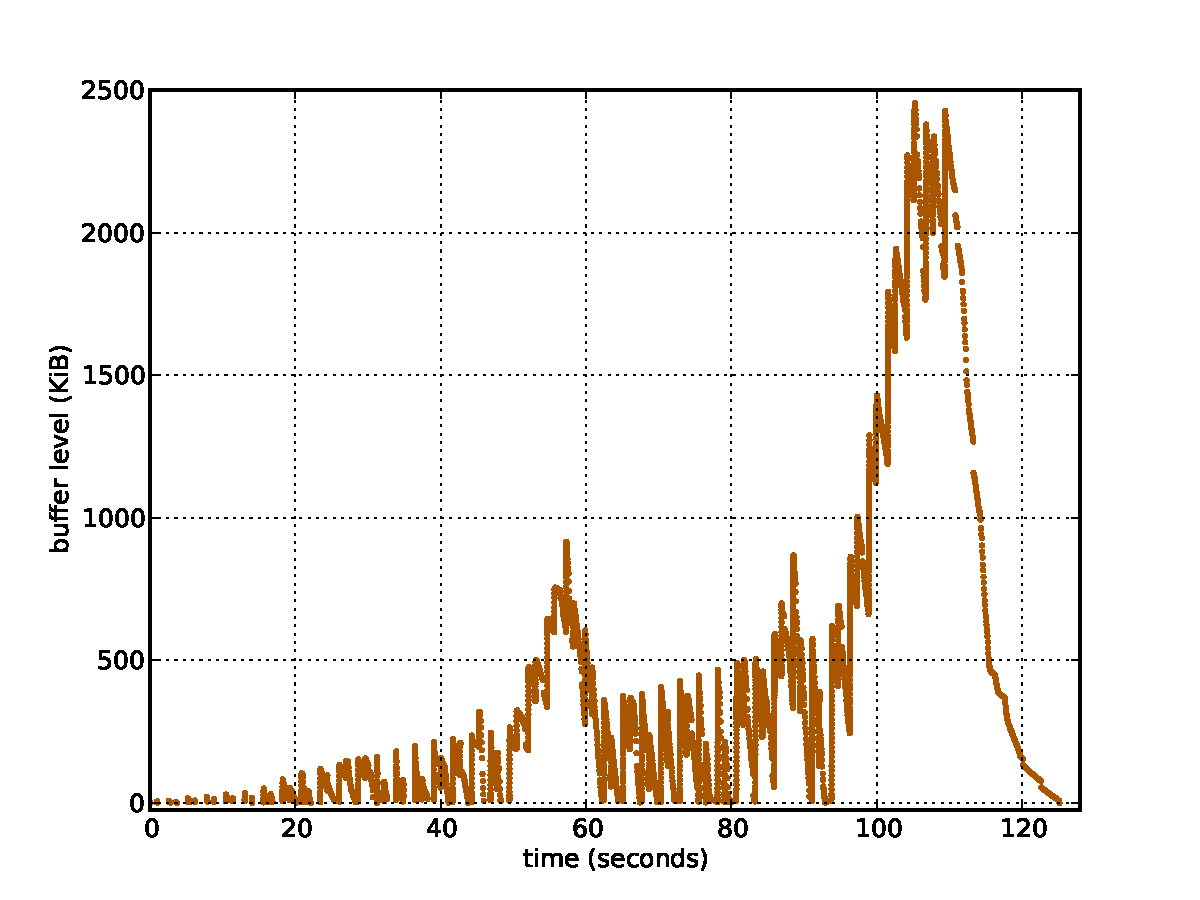
\includegraphics[width=0.9\textwidth]{images/bufferlevel-stall-new.pdf}
    \caption{Buffer fill level with null strategy; \SI{33}{\second} total stalling.}
    \label{c3:fig:bufferlevel-stall}
\end{figure}

Figure~\ref{c3:fig:bufferlevel-stall} depicts an exemplary time series diagram of the contents of a video buffer using this strategy with a transmission rate only slightly above the video stream's rate. The buffer frequently drops down to zero forcing a short stall. According to the presented related work on the \gls{QoE} impact of stalling frequency in comparison to the length of stalls \cite{6123395}, this is the worst possible scenario for a person watching the stream.


%%
\subsubsection{Threshold Strategies}

Instead of instantly restarting playback, a lower threshold can be introduced. Only after a certain buffer fill level threshold has been surpassed, playback will be started. Thresholds can be set independently for the initial playback delay and stalls, with the initial playback delay generally set to be higher.

The threshold can be chosen in a number of ways. It can either be an absolute data volume, a buffered video duration. The latter is much more suited for variable bitrate videos as it automatically adapts itself to the current bitrate. A third option is to buffer for a certain amount of real time -- this can be seen as threshold -- and starting playback after that period regardless of the volume of the buffer. Additionally, the threshold could also either be set to a constant value or dynamically chosen according to the expected network \gls{QoS}.

Besides this single-threshold strategy, a two-threshold strategy might make more sense for segment-based streaming. In addition to the lower threshold, an upper threshold is introduced. When reached, no new segments will be requested until the buffer arrives at the lower threshold again.  To achieve an hysteresis effect a third threshold, somewhere between the lower and upper bound, can also be introduced. Through this, the maximum buffer size can also be controlled. This is important in situations with hard limits on available memory. Mobile devices come to mind here.

\begin{figure}[htb]
    \centering
    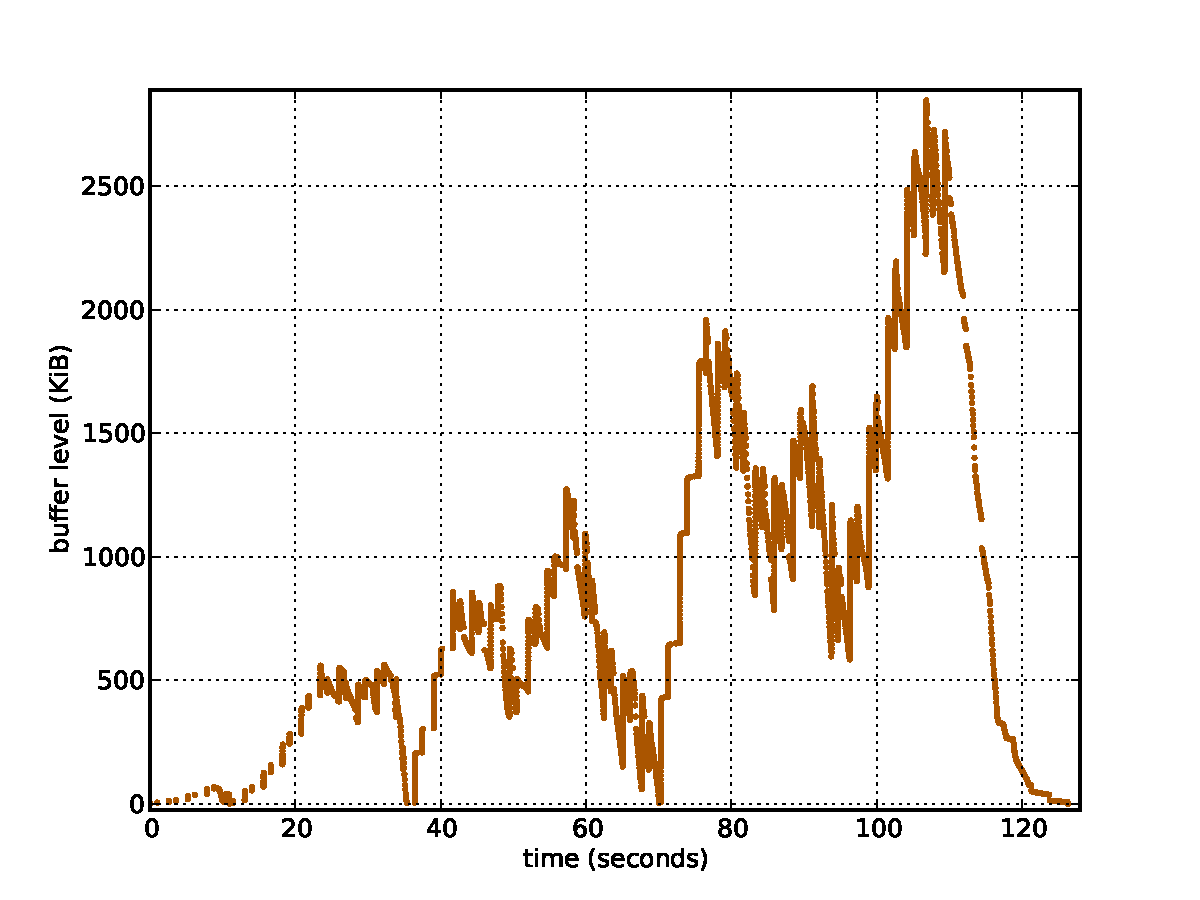
\includegraphics[width=0.9\textwidth]{images/bufferlevel-flash-new.pdf}
    \caption{Sample buffer fill level for a \SI{2}{\second} and \SI{5}{\second} buffered video duration threshold strategy; \SI{34}{\second} total stalling.}
    \label{c3:fig:bufferlevel-flash}
\end{figure}

An example buffer diagram is displayed in Figure~\ref{c3:fig:bufferlevel-flash}. In this case, the initial delay was controlled by a buffered video duration threshold of \SI{2}{\second} and a resume condition also based on buffered video duration but with a \SI{5}{\second} threshold. The strategy produces noticeable less stalls than the null strategy but slightly increases the total stalling time.


%%
\subsubsection{Pacing Strategies}

For segment-based \gls{HTTP} streaming, a two-threshold strategy is not the only supplemental option on top of simple streaming. Here, the controller can pace the request of future segments to match the overall, or the current video bitrate. A safety margin can also be factored in to even out short time fluctuations of either the transmission or the video bitrate. For example, the controller would request segments with an overall transmission rate of 1.25 times the video bitrate. The pacing rate can either be statically chosen in advance or can be calculated dynamically based on current or future conditions. The latter leads to predictive strategies.

%%
\subsubsection{Predictive Strategies}

In predictive strategies, knowledge of the future of the streaming process is used by the controller to adjust the start/stop and segment retrieval conditions. Instead of global knowledge, heuristics can instead attempt to approximate a future state.

A very simple predictive approach is to prolong the initial delay to the point, that no intermediate buffer underrun and thus no stall will occur. With global knowledge, the controller can start the stream at the earliest possible point in time, thus minimizing the total stalling time while still having only the initial delay.

\begin{figure}[htb]
    \centering
    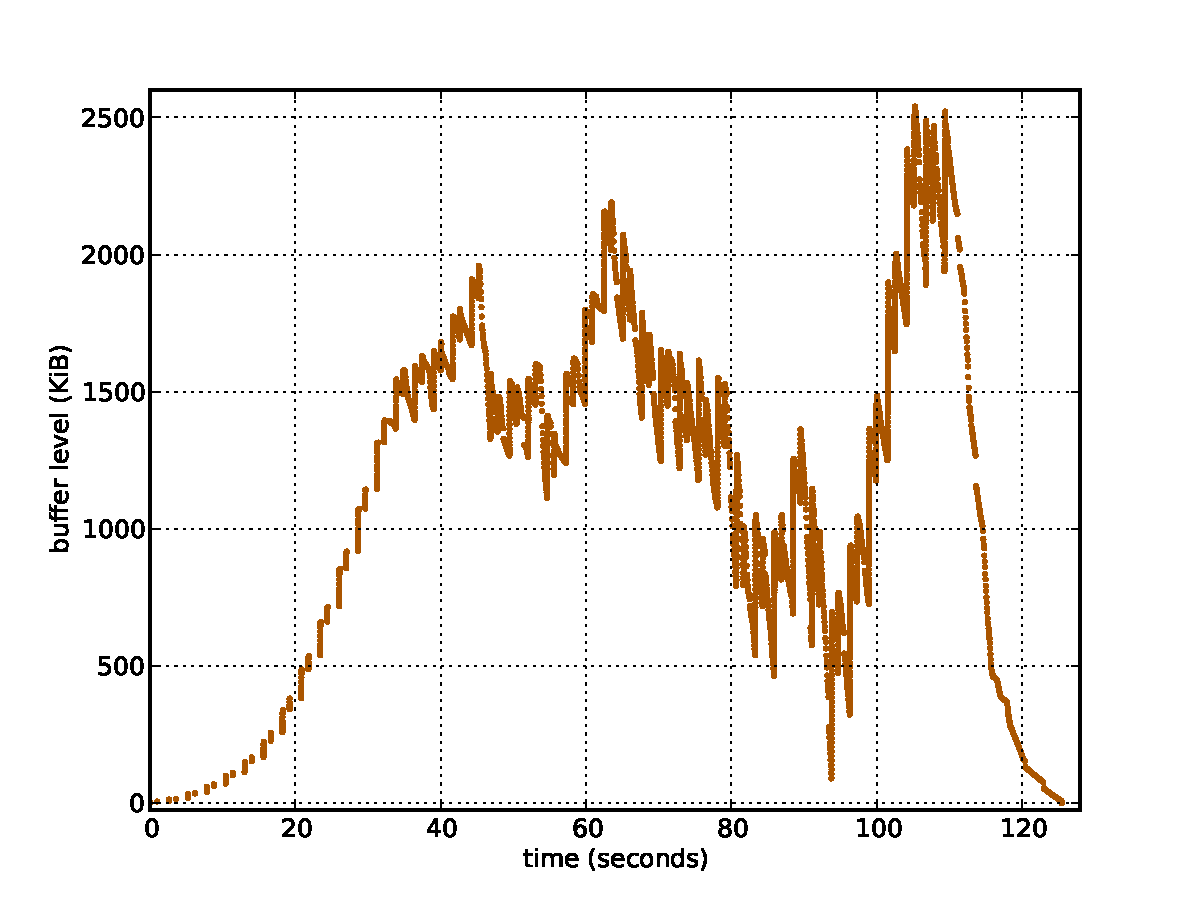
\includegraphics[width=0.9\textwidth]{images/bufferlevel-startdelay-new.pdf}
    \caption{Sample Buffer fill level for the delayed playback model, \SI{33}{\second} total stalling.}
    \label{c3:fig:bufferlevel-startdelay}
\end{figure}

Figure~\ref{c3:fig:bufferlevel-startdelay} depicts the time series of a sample implementation of this delayed playback predictive strategy with all necessary stalling occurring upfront.


%%
\subsubsection{Adaptive Strategies}

Most strategies for adaptive streaming are an extension of both the threshold as well as the pacing strategy. However, instead of a simple transmit-or-no-transmit ruleset, they can make much more fine-grained adjustments. The quality of the stream segment to be requested will be chosen, depending on the current fill level and drain rate of the buffer. This makes a trade off between maintaining a certain quality level and putting up with increased waiting times, and dropping the quality to a level sustainable at the current transmission rate.


\subsubsection{Real World Implementation Examples}

Actual streaming player implementations often do not implement only one of these strategies, but rather combine ideas from several. Herein, thresholds are often set arbitrarily through the implementor's best practices and not empirically evaluated, often making a trade-off between user perceivable quality and resulting server load. In general, every streaming service practically implements its own playback strategies. This section describes three example applications.

%%
\paragraph{2011 YouTube Flash Player Buffering Strategy}

Google's video streaming site YouTube is constantly changing its appearance and technical makeup. In recent years, YouTube streams are delivered by one of three players: The Website's Flash player, a browser-integrated HTML5-based player, or custom player implementations in mobile phones, set-top boxes and similar devices. Here, the Flash-based variant used in 2011 is described.

This player used a single threshold strategy with different threshold values for the initial delay and any subsequent stalls. The values were already described in Figure~\ref{c3:fig:bufferlevel-flash}. This model assumes sufficient network conditions in the beginning, requiring only a short initial playback delay to pre-fill the playback buffer. If, however, stalling occurs, then it will buffer longer to keep the stalling frequency down.

\begin{table}[htb]
    % increase table row spacing, adjust to taste
    %\renewcommand{\arraystretch}{1.3}
    \caption{Transmission Related Parameters from YouTube's Video URL Setup}
    \label{c3:tbl:yturl}
    \centering
    \begin{tabu}{|X[l]|X[p]|}
        \hline
        URL Part & Description \\ \hline
        \texttt{v$\alpha$.lscache$\beta$.c.youtube.com} &  Cache server involved in the delivery.\\
        \texttt{algorithm=throttle-factor} and \texttt{burst=40} and \texttt{factor=1.25} & Indicates initial burst plus block sending configuration. \\
        \texttt{ratebypass=yes} & Parameter to indicate no rate limiting.\\ \hline
    \end{tabu}
\end{table}

Furthermore, YouTube employs a proprietary pacing mechanism outside of the control of the streaming player. This is hinted at in the encoding of the \glspl{URL} of the video files and enforced by the video file cache server. Some of those not user-changeable parameters are described in Table~\ref{c3:tbl:yturl}. The pacing was in effect for all videos below high definition resolution, but has since then been extended to include all video files. 

\begin{figure}[htbp]
% used yt-delay/hPUGNCIozp0_delay_100 2, spyder with matplotlib config patch
    \centering
        \begin{subfigure}[b]{0.90\textwidth}
                \centering
                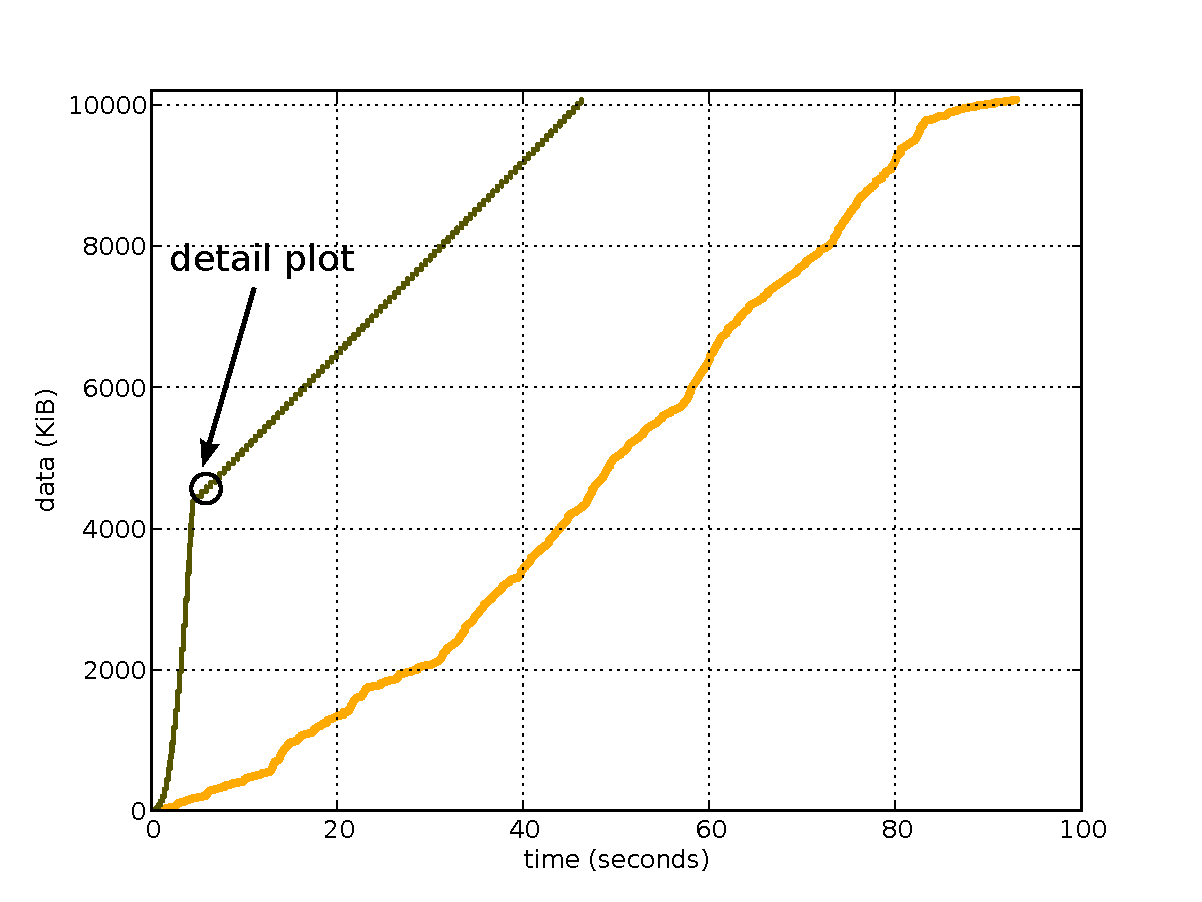
\includegraphics[width=\textwidth]{images/blocktransfer-mod.pdf}
                \caption{Overall graph.}
                \label{c3:fig:blocktransfer-overall}
        \end{subfigure}

        \begin{subfigure}[b]{0.90\textwidth}
                \centering
                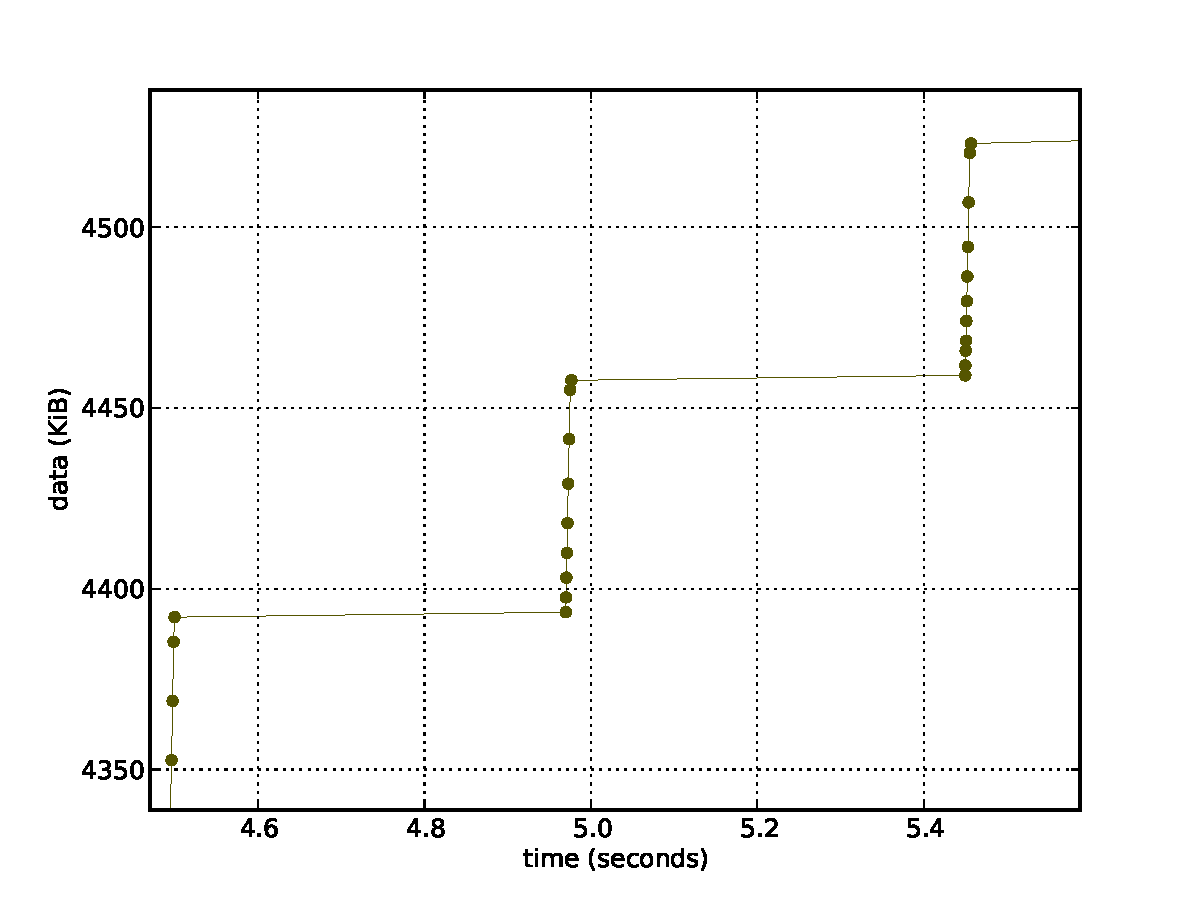
\includegraphics[width=\textwidth]{images/blocktransferdetail.pdf}
                \caption{Detail plot of the rate-limited block-sending phase.}
                \label{c3:fig:blocktransfer-detail}
        \end{subfigure}
\caption{Comparison of downloaded and consumed data volume revealing the pacing mechanism used by YouTube.}
\label{c3:fig:blocktransfer}
\end{figure}


The throttling method, also observed in \cite{alcock2011afcyt}, limits the transmission to a rate slightly above the average media bitrate, measurements and the \gls{URL} scheme indicates this to be a factor of the video bitrate of $1.25$. The rate limit is not constant, instead a ON-OFF block-sending scheme is facilitated. The scheme transmits short packet bursts, typically \SI{64}{\kibi\byte} in size, followed by long pauses as seen in Figure~\ref{c3:fig:blocktransfer}. The pause length between two bursts is set dynamically to reach the targeted bitrate on a larger time scale. The initial phase of the stream transmission is conducted unthrottled at line speed, presumably to allow for some pre-buffering to occur at the client media player. A possible reason for this server-side pacing is to avoid load spikes, with the added side effect of keeping the clients' buffer sizes in check.



%%
\paragraph{Firefox's HTML5 Player Strategy}

Video streaming can also be directly conducted with the Web browser, through the use of a HTML5 canvas element. The \gls{W3C} specifies the default technical process of HTMl5 video streaming in \cite{html5video} and essentially suggests a predictive strategy. Herein, the Web browser should estimate and correlate the transmission rate to the video bitrate. A property called ``autoplay'' uses this definition to start  playback of the associated video \enquote{as soon as it can do so without stopping}. The HTML5 strategy also allows to limit the buffer size through transmission pacing, negotiated with the server, and appropriately timed range requests.

The open-source Firefox browser represents an implementation of this specification and substantiates it further. The description of this strategy is based on Firefox's version 4.0 released in March 2011. Because it is an online algorithm which does not have global knowledge of the video and transmission speeds of any point in the future it has to estimate these.
To estimate the current and future rates, the moving average of the transmission rate $s_{MA}$ and the video bitrate $v_{MA}$ are calculated. The condition $c$ Firefox uses to start and resume the playback process is given in Algorithm~\ref{c3:alg:firefox}, with the buffered video duration $b_b$, and the duration spent buffering $b_T$.

\begin{algorithm}[htb]
    \centering
    \begin{algorithmic}
        \IF {$s_{MA} > v_{MA}$} 
          \STATE $c \gets ( b_b=20s \lor b_T=20s )$
        \ELSE
          \STATE $c \gets ( b_b=30s \lor b_T=30s )$
        \ENDIF 
    \end{algorithmic}
    \caption{Firefox playback (re-)start decision algorithm.}
    \label{c3:alg:firefox}
\end{algorithm}

 \begin{figure}[htb]
    \centering
    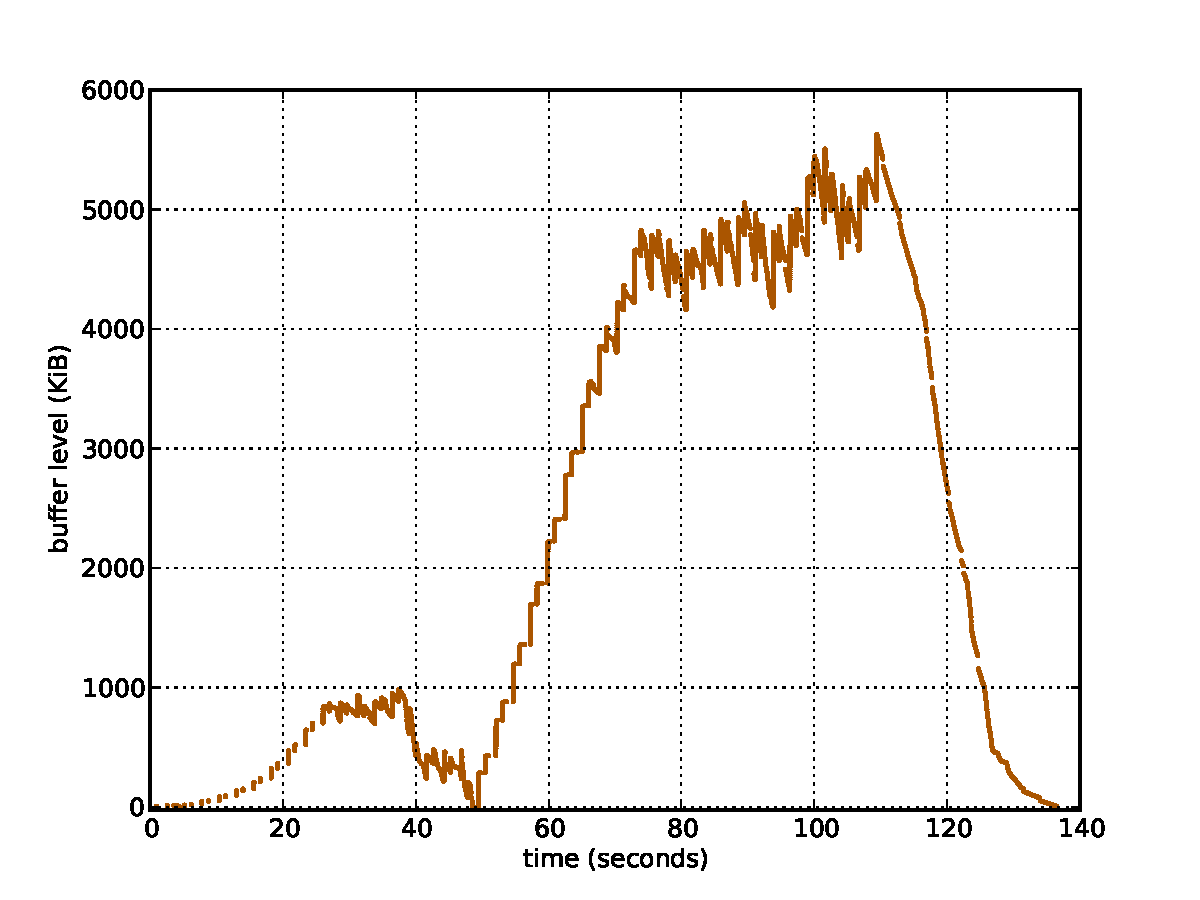
\includegraphics[width=0.9\textwidth]{images/bufferlevel-firefox-new.pdf}
    \caption{Sample buffer fill level for the Firefox 4 strategy, \SI{44}{\second} total stalling.}
    \label{c3:fig:bufferlevel-firefox}
\end{figure}


This approach is quite conservative and trades off long stalling periods for fewer stalls. The test case for our model is shown in Figure \ref{c3:fig:bufferlevel-firefox}. The playback starts only after a long waiting period and intermittent stalls cause a long buffering period. 
Due to the longer overall stalling time the player needs to buffer more data than other strategies. This may make it unsuitable for devices with sparse amounts of memory, e.g. mobile phones. On the other hand, could a large buffer also increase the chance of continuous playback in such scenarios with bad \gls{QoS}.


\paragraph{Adaptive streaming strategies}

Implementations for adaptive streaming players are again mostly proprietary and their behavior has to be derived from measurements. This is even true for adaptive streaming protocols, which have open specifications as these generally do not specify the player's behavior.

Microsoft's Silverlight player's strategy is described in \cite{BLTJ:BLTJ20505}. It employs a two-threshold model and rate estimations. When on of the thresholds is reached, the quality will be adjusted by one step upwards or downwards as long as the transmission rate is sufficient.

The buffering behavior of further protocol variants, including Adobe's \gls{HTTP} Dynamic Streaming, Apple's \gls{HTTP} Live Streaming and a sample implementation of \gls{DASH}, are investigated in \cite{Muller:2012:EDA:2151677.2151686,akhshabi2011experimental}.




% \begin{itemize}
% \item The player has been buffering data for at least 30 seconds.
% \item The player has already buffered an amount of data corresponding to 30 seconds of video.
% \item The video download has been completed.
% \item The moving average of the transmission rate is larger than the moving average of the video bitrate and the player has a safety buffer with 20 seconds of video data.
% \end{itemize}

% \begin{table}[htb]
%     \caption{Variables involved in buffering decisions.}
%     \label{c3:tbl:buffvars}
%     \centering
%     \begin{tabu}{|l|X[p]|} 
%     \hline
%     Variable & Description \\ \hline
%     $s_{MA}$ & Moving average of the transmission speed. \\
%     $v_{MA}$ & Moving average of the video bitrate. \\ 
%     $c$   & Condition upon which to start/resume playback. \\
%     $b_b$    & Amount of video data the buffer contains. \\
%     $b_T$    & Amount of time spent in non-playing buffering state. \\ \hline
%     \end{tabu}
% \end{table}

% used yt-delay/hPUGNCIozp0_delay_2500 1, spyder, color #aa5500
% data
% start delay 33s 
% flash 33.82s
% stalling 32.68s
% html5 as implemented in firefox 44s


%Which offers better quality to users? Some approaches (TODO: refs and explain how)

% Longer waiting time but very few stops. Stalling model definitely the shortest waiting time but stops too frequent with insufficient network conditions, i.e. can not really be used. Delayed playback requires total knowledge not available beforehand. Can maybe used with reduced information, bandwidth estimation, but this is essentially HTML5/Firefox.




%``application comfort'' time to skip, ...
%\subsubsection{Unreliable Streaming Metrics}
%... and why they mostly do not work / are not applicable.




%%%%%%%%%%%%%%%%%%%%%%%%%%%%%%%%%%%%%%%%%%%%%%%%%%%%%%%%%%%%%%%%%%%%%%%%%%%%%%%%
\section{Summary}
\label{c4:sec:conclusion}
In this paper, we take a look at the signaling behavior of devices in an operational \ac{3G} mobile network providing Internet access. Our focus does not lie on the wireless or user-oriented parts of the network, but on signaling in the core network. To the best of our knowledge, this paper is the first to offer a core network perspective on signaling. We give a \ac{GPRS} and \ac{UMTS} network primer, and introduce \ac{GTP} tunnel management, explaining the causes and actions within the network. Our evaluation is based on a week long data set acquired in the core network of an Austrian mobile operator.

% We now go back to the case of Angry Birds which was much quoted for causing excessive radio signaling at one point in time. 
In our observation of core network signaling involving PDP Contexts and their management, we looked at the effect of device types and operating systems on the duration of GTP tunnels. We can conclude that the distribution of tunnel durations in our evaluated dataset is dominated by smartphones. This is contrary to the conventional idea that a larger volume of user plane traffic also leads to an increase of signaling. In our dataset, this would mean that 3G dongles would cause most signaling, which is definitely not the case. In this aspect, our findings support the stories of the casual game ``Angry Birds'' causing signaling storms in mobile networks by frequently downloading small ads, each small download resulting in disproportionate amounts of signaling load being generated. We conjecture from our results that measures taken to improve the radio interface control plane such as Fast Dormancy can have the converse effects in the core, as they could increase the tunnel churn.

All in all, our paper shows that operators can determine which type of device has the most influence on the current network infrastructure by looking at and comparing tunnel duration distributions. %Moreover, if a load situation occurs in the core network, the operator can decide which devices are the root cause and take appropriate measures. 
This investigations can also lead to better network planning that is more aware of the control plane by providing the necessary tools to identify probable causes for control plane activity. Lastly, we hope to raises some awareness with programmers about the potential unintended side effects their application traffic patterns can cause.

\subsection{Future Endeavors}

This paper serves as an introduction to the topic of the 3G core network control plane, and therefore provides only some initial insights into the actual signaling dynamics. Therefore, we would like to expand our evaluations, as there are several  angles not investigated so far that could prove worthwhile.

To get a grasp of the imposed load on the network as well as the involved network nodes, a calculation of the sizes of the tunneling messages was already hinted at. To improve on this naive attempt, actual numbers on the message sizes and involved \acp{IE} could be recorded in future traces. Having correct signaling traffic volume data still does not reveal the processing load on core network elements. We plan to improve our methodology in this respect by taking at a look at how long it takes for the gateway nodes to process \ac{GTP} messages with respect to the current amount of user traffic and signaling. \ac{GTP} tunnels also cause a certain amount of overhead through additional headers and potential fragmentation of the user traffic, providing another investigation venue for the future (albeit more oriented towards user-plane IP traffic). 

Furthermore, besides the device-based classification, a differentiation based on the user traffic dynamics and correlation to signaling is planned. When looking closer at specific users, the mobility behavior also comes to mind. To investigate this, we intend to take a closer look at the occurring tunnel update messages as evidence, amongst others for mobility.

We also look forward to searching for multiple active tunnels per device. As discussed previously, the \textit{Secondary PDP Context Activation Procedure} enables devices to establish up to ten additional tunnels attributed with a different, higher QoS level, if the network supports this. The additional load of managing and holding multiple tunnels plus the displacement of other, ``lower-quality'' traffic could prove to be an interesting investigation. Initial observations indicate that this feature is rarely used today by very few types of devices, but it will be of increased interest in the face of ongoing LTE/EPS deployments, whose specifications expand upon this secondary tunnel concept.



%%%%%%%%%%%%%%%%%%%%%%%%%%%%%%%%%%%%%%%%%%%%%%%%%%%%%%%%%%%%%%%%%%%%%%%%%%%%%%%%
%%% CoNEXT Conclusion Starts here

In this paper, we took a look at the signaling behavior of devices in an operational \ac{3G} mobile network providing Internet access. Our focus does not lie on the wireless or user-oriented parts of the network, but on signaling in the core network. To the best of our knowledge, this paper is the first to offer an in-depth core network perspective on signaling. We gave a \ac{GPRS} and \ac{UMTS} network primer, and introduced \ac{GTP} tunnel management and evaluated a week long data set recorded in the core network of an Austrian mobile operator.

In our observation of core network signaling involving \ac{PDP} Contexts and their management, we looked at the effect of device types and operating systems on the duration of \ac{GTP} tunnels. We can conclude that the distribution of tunnel durations in our evaluated dataset is dominated by smartphones. This is contrary to the conventional idea that a larger volume of user plane traffic also leads to an increase of signaling. In our dataset, this would mean that 3G dongles would cause most signaling, which is definitely not the case. Our paper shows that operators can determine which type of device has the most influence on the current network infrastructure by looking at and comparing tunnel duration distributions.

For additional load investigations we also looked at the inter-arrival and processing time of tunnels and found further evidence of radio and diurnal effects influencing the core network. With this data in mind, an initial M/M/$\infty$ queue was created to model load occurring at the \ac{GGSN} with simple stationary analysis. This also serves a basis for future more detailed models.

We think that this investigation and load modeling can lead to better network planning: Being more aware of the control plane provides the necessary tools to identify probable causes for control plane activity. We would also like to expand our evaluations, as there are several angles not investigated so far that could prove worthwhile. This includes an examination of the exact number and size of signaling messages flowing through the core, a more detailed picture of the processing load these messages induce at the \ac{GGSN}, and an evolved model. Furthermore, a differential analysis of our data compared to a newer dataset (potentially including \ac{LTE} access) could really prove worthwhile.

